\documentclass[a4paper,12pt]{report}

\usepackage{amssymb}
\usepackage{latexsym}
\usepackage{amsmath}
\usepackage{amsthm}
\usepackage{wrapfig}
\usepackage{geometry}
\usepackage{pstricks}
\usepackage{pst-node,pst-tree}
\usepackage{pst-rel-points}
\usepackage{flexiprogram}
\geometry{verbose,a4paper,tmargin=15mm,bmargin=30mm,lmargin=30mm,rmargin=20mm}
\usepackage{graphics}
\usepackage{framed}
% \usepackage{fancyheadings}
\usepackage{cite}
\usepackage{url}
\usepackage{array}
\usepackage{multirow}
\usepackage{verbatim}
\usepackage{graphicx}
\usepackage{multicol}
\usepackage{fancyhdr}
\usepackage{epsfig}
\usepackage{setspace}
\usepackage{listings}
\usepackage{subfigure}
\usepackage{framed}
\usepackage{tabularx}
\usepackage{epstopdf}
\usepackage{color}
\usepackage{longtable}
\usepackage[sand]{optional}

% % \usepackage{algpseudocode}
% \usepackage{algorithm}
% \usepackage{algorithmic}

\newtheorem{example}{Example}
\newtheorem{definition}{Definition}
\lstset{language=C,basicstyle=\footnotesize\ttfamily ,columns=fullflexible,keywordstyle=,morekeywords=}



%\begin{comment}
\usepackage[colorlinks,breaklinks=true]{hyperref}% hyperref should be the last package to be included, and perhaps there  should be one line gap between entries of bibliography 

%below block all concerns package hyperref
\hypersetup{
	hypertexnames=false,
	pdftitle={Field Sensitive Analysis Implementation and Improvements},
	pdfauthor={P Vinay Kumar Reddy},
	pdfkeywords={},
	bookmarksnumbered,
% 	bookmarks=true,
% 	bookmarksopen=true,
	pdfstartview={FitH},
	colorlinks=true,
	urlcolor=black,
	linkcolor=black,%: Color for normal internal links
	anchorcolor=black,%: Color for anchor text.
	citecolor=black,%: Color for bibliographical citations in text
	filecolor=black,%: Color for URLs which open local files
%	pagecolor=blue,%: Color for links to other pages
}%

% \usepackage{multibib}

% \currentpdfbookmark

%---------------------------------end of packages----------------------------------------------------

\setlength{\topmargin}{-13mm}
\setlength{\headheight}{6mm}
\setlength{\headsep}{7mm}
\setlength{\textheight}{245mm}
%\setlength{\oddsidemargin}{0.37in}
\newpage
%\setlength{\evensidemargin}{0in}
\setlength{\textwidth}{150mm}
\setlength{\marginparwidth}{0.5in}
\renewcommand{\baselinestretch}{2}



\pagestyle{fancy}
\setlength{\headheight}{35pt}
\fancyhead{}
\fancyfoot{}
\renewcommand{\headrulewidth}{0pt}
\renewcommand{\footrulewidth}{0pt}
\setlength\fboxsep{1pt}
\setlength\fboxrule{0.25pt}
%\theoremstyle{definition}
\newtheorem{mydef}{Definition}[chapter]

\renewcommand\lstlistingname{Program}%                     default is Listing
\renewcommand\lstlistlistingname{List of Programs}%        default is Listings
\addtolength{\evensidemargin}{-.875in}
\begin{document}
\pagenumbering{roman}
\fancyfoot[CO]{\thepage}
\cleardoublepage



\addtocontents{toc}{\protect{\pdfbookmark[0]{Table Of Contents}{toc}}}
\addtocontents{lof}{\protect{\pdfbookmark[0]{List of Figures}{lof}}}
% \addtocontents{lot}{\protect{\pdfbookmark[0]{\contentsname}{lot}}}
%*******************************************************************************
%-------------------------Start of my variables-----------------------------------------------
\newcommand{\cmt}[1]{}
\newcommand{\p}{\ensuremath{p}}
\newcommand{\q}{\ensuremath{q}}
\newcommand{\s}{\ensuremath{s}}
\newcommand{\myr}{\ensuremath{r}}
\newcommand{\F}{\ensuremath{F}}
\newcommand{\I}{\ensuremath{I}}
\newcommand{\x}{\ensuremath{x}}
\newcommand{\y}{\ensuremath{y}}
\newcommand{\f}{\ensuremath{f}}
\newcommand{\g}{\ensuremath{g}}
\newcommand{\Left}{\ensuremath{Left}}
\newcommand{\Right}{\ensuremath{Right}}
\newcommand{\Parent}{\ensuremath{Parent}}  
\newcommand{\merge}{\ensuremath{\mathrm{merge}}}


\newcommand{\num}[1]{\ensuremath{|#1|}}
\newcommand{\drct}{\ensuremath{D}}
\newcommand{\indrct}{\ensuremath{I}}
\newcommand{\fieldD}[2]{\ensuremath{{#1}_{#2}^\drct}}
\newcommand{\fieldI}[3]{\ensuremath{{#1}_{#2}^{\indrct#3}}}
\newcommand{\alias}[1]{\ensuremath{{#1}^{\dag}}}
\newcommand{\aliasinfo}[1]{\ensuremath{\{\myr | \myr = #1 \vee \epsilon \in D_F^{\din}[\myr,#1] \vee \epsilon \in D_F^{\din}[#1, \myr] \}}}
%\newcommand{\myT}{\mbox{\tt T}}
\newcommand{\myL}{\mbox{\tt L}}
%\newcommand{\R}{\mbox{\tt R}}
\newcommand{\false}{\textbf{False}}
\newcommand{\true}{\textbf{True}}
\newcommand{\subC}{\mbox{\scalebox{0.6}{\Cycle}}}
\newcommand{\subD}{\mbox{\scalebox{0.6}{\Dag}}}

\newcommand{\dout}{\mbox{\footnotesize\em out}}
\newcommand{\din}{\mbox{\footnotesize\em in}}
\newcommand{\dkill}{\mbox{\footnotesize\em kill}}
\newcommand{\dgen}{\mbox{\footnotesize\em gen}}

\newcommand{\GenC}[1]{\ensuremath{{#1}_{\subC}^{\dgen}}}
\newcommand{\GenD}[1]{\ensuremath{{#1}_{\subD}^{\dgen}}}
\newcommand{\KillC}[1]{\ensuremath{{#1}_{\subC}^{\dkill}}}
\newcommand{\KillD}[1]{\ensuremath{{#1}_{\subD}^{\dkill}}}
\newcommand{\InC}[1]{\ensuremath{{#1}_{\subC}^{\din}}}
\newcommand{\InD}[1]{\ensuremath{{#1}_{\subD}^{\din}}}
\newcommand{\OutC}[1]{\ensuremath{{#1}_{\subC}^{\dout}}}
\newcommand{\OutD}[1]{\ensuremath{{#1}_{\subD}^{\dout}}}

\newcommand{\Tree}{{\tt Tree}}   %tt stands for typewriter font
\newcommand{\Dag}{{\tt Dag}}
\newcommand{\Cycle}{{\tt Cycle}}

\newcommand{\upath}{\ensuremath{\mathcal{U}}}
\newcommand{\heap}{\ensuremath{\mathcal{H}}}
\newcommand{\fields}{\ensuremath{\mathcal{F}}}
\newcommand{\shape}{\mbox{shape}}
\newcommand{\nat}{\ensuremath{\mathcal{N}}}

\newcommand{\epsilonset}{\ensuremath{\{\epsilon\}}}
\newcommand{\epsilonpairset}{\ensuremath{\{\epsilon,\epsilon\}}}

\newcommand{\project}[2]{\ensuremath{#1\triangleright\!\!#2}}
\newcommand{\anysup}{\ensuremath{\ast}}

\newcommand{\DFM}[2]{\ensuremath{D_F[#1,#2]}}
\newcommand{\IFM}[2]{\ensuremath{I_F[#1,#2]}}

\newcommand{\remOne}[2]{\ensuremath{#1 \ominus #2}}
\newcommand{\remAll}[2]{\ensuremath{#1\uminus #2}}



%-------------------------End of my variables----------------------------------------------

\titlepage
\begin{center}
\noindent {\bf{\Large{\sc Field Sensitive Shape Analysis: Implementation and Improvements}}}\\
\end{center}
\vspace{50mm}
\begin{center}
{\it by}\\
\vspace{5mm}
{\bf{\Large P.Vinay Kumar Reddy}}\\
\end{center}
\vspace{45mm}
%\begin{figure}[h]
%\centering
% \begin{center}
{\centering {
\includegraphics[width=.3\linewidth]{diagrams/logoMain.eps}}\par}
% \end{center}
%\caption{}
%\end{figure}
\begin{center}
\vspace{3mm}
{\bf {\large {\sc Department of Computer Science and Engineering}}}\\
\vspace{2mm}
{\bf {\large INDIAN INSTITUTE OF TECHNOLOGY KANPUR}}\\
\vspace{3mm}
{\textbf{ June, 2012}}\\
\end{center}



\newpage

\titlepage
\thispagestyle{empty}
\begin{center}
\noindent {\bf{\Large{\sc Field Sensitive Shape Analysis: Implementation and Improvements}}}\\
\end{center}\vspace{15mm}
\begin{center}
{\it{A Thesis Submitted}}\\
{\it{in Partial Fulfillment of the Requirements}}\\
{\it{for the Degree of}}\\

{\bf {\large Master of Technology (M.Tech)}}\\
\vspace{15mm}

{\it{by}} \\
{\bf{\large P.Vinay Kumar Reddy}}\\

\vspace{1cm}
{\it{Supervised By}} \\
%\vspace{.5cm}
%\hspace{.05cm} 
{\large \bf {Dr. Amey Karkare}}\\
\end{center}
\vspace{8mm}
\begin{figure}[h] 
%\hspace{6cm}
%\vspace{5cm}
{\centering {
\includegraphics[width=.3\linewidth]{diagrams/logoMain.eps}}\par}
\end{figure} 
\begin{center}
\vspace{3mm}
{\bf {\large {\sc Department of Computer Science and Engineering}}}\\
\vspace{2mm}
{\bf {\large INDIAN INSTITUTE OF TECHNOLOGY KANPUR}}\\
\vspace{3mm}
{\textbf{June, 2012}}
\end{center}

		% First Inner Page
\newpage
%\phantomsection\addcontentsline{toc}{chapter}{Certificate}
\setcounter{page}{2}
% %\vspace*{\fill}
\vspace*{1.0in}
\begin{center}
\begin{large}
{\bf CERTIFICATE}
\end{large}
\end{center}
\vskip 2cm
It is certified that the work contained in this thesis entitled \\``{{\textit{Field Sensitive Shape Analysis: Implementation and Improvements}}}'',\\ by {{\textit{P.Vinay Kumar Reddy(Roll No. 10111026)}}}, has been carried out under my \\supervision and that this work has not been submitted elsewhere for a degree.
\vskip 1in
\begin{flushleft}
		\hspace*{5.8cm}{\hrulefill}\\
		\hspace*{5.8cm}(Dr. Amey Karkare)\\
		\hspace*{5.8cm}Department of Computer Science and Engineering,\\ 
		\hspace*{5.8cm}Indian Institute of Technology Kanpur\\
		\hspace*{5.8cm}Kanpur-208016
\end{flushleft}
June, 2012

%\vspace*{\fill}
	

\includegraphics{InitialPages/vinay_scan.eps}
% \newpage
%\phantomsection\addcontentsline{toc}{chapter}{Abstract}
%\phantomsection\addcontentsline{toc}{chapter}{Acknowledgements}

\setstretch{1.5} 
\begin{center}
\begin{large}
{\it{\bf ACKNOWLEDGMENTS} }
\end{large}
\end{center} 
I take this opportunity to thank my thesis guide \textbf{Dr. Amey Karkare} for his invaluable support and
guidance. He has been utmost patient and helped me throughout in completion of my work. I express my gratitude
to the faculty and staff of the Department of CSE for the beautiful academic environment they have created here.

I would like to thank \textbf{Mr. Sandeep Dasgupta} for his immense support and invaluable suggestions that I have
received from him. 

I would also like to thank all my friends of Mtech 2010 Batch and especially Anvesh, Ashendra, Chitti Babu, Keerthi Kumar and Saravana 
for making my stay at IIT Kanpur truly special. 

Finally, I wish to extend my thanks to my parents, my brother for their support and encouragement.
Every effort has been made to give credit where it is due for the material contained
here in. If inadvertently I have omitted giving credit to anyone, I apologize and express
my gratitude for their contribution to this work

\vskip 4mm
\begin{flushright}
\textit{\textbf{P. Vinay Kumar Reddy}}
\end{flushright}

\newpage


\vspace*{\fill}

\begin{center}
{\it Dedicated to}\\
{\it my parents,my brother and my friends.}
\end{center}

\vspace*{\fill}



\setstretch{1.2}     %space between lines

\newpage
\opt{sand}{\pdfbookmark[1]{Abstract}{abstract}}
%\vspace*{\fill}
\vspace*{1.0in}

\begin{center}
\begin{large}
{\bf Abstract}
\end{large}
\end{center}

Shape Analysis refers to a class of techniques used to analyze heap data structures. Several algorithms have been proposed in literature
about shape analysis. These algorithms differ in the trade off they have between speed and accuracy.
    
  In this thesis we have implemented and proposed enhancements for a field sensitive shape analysis approach. These enhancements involve modification of data flow values, and intelligent
way of storing the same which makes the analysis more precise and memory efficient. This work also proposes an analysis namely \emph{Subset Based Analysis}
which infers more precise shapes depending upon which field pointers are actually accessed in a function. To handle functions we have developed
a new method for interprocedural analysis called \emph{Shape Sensitive Analysis}. This is a middle way between Context Sensitive and Context Insensitive Interprocedural Analysis.
We have implemented this analysis as a plugin for gcc 4.5.0 and the results for the same are presented. 




\tableofcontents

\listoffigures


\newpage
\pagenumbering{arabic}
\fancyhead[RO]{\thepage}
\fancyhead[LO]{\slshape \leftmark}
\fancyfoot[CO]{}
\renewcommand{\headrulewidth}{0.5pt}
\noindent
% %*********************************************************************
\chapter{Introduction\label{intro}}
\chapter{Introduction}
\label{ch:Intro}
In the recent arena of parallel architectures (multi-cores,
GPUs, etc.), software side lags behind hardware. This is due to the reason that dealing with 
parallelism adds a new dimension to the design of programs, therefore 
makes it complex. One approach for efficient parallelization of programs is to explicitly 
induce parallelism. It includes designing of concurrent programming languages like Go, X10 etc., 
libraries, APIs like POSIX, OpenMP, Message 
Passing Interface(MPI) etc. The main advantage of such approach is that it gives simple and clear directions to the 
compiler to parallelize the code. But the main drawbacks of such approach is that the degree of parallelism totally depends upon 
the efficiency of programmer and imposing external parallelism turns the code into legacy one. 
The other approach is to automatically 
parallelizing sequential programs by compiler which extract parallelism 
without violating correctness. This is a key step in increasing
the performance and efficiency. 
%
\section{Motivation}
Over the past years, lot of work has been done on automatically 
parallelizing sequential programs. These approaches have mainly 
been developed for programs having only static data structures 
(fixed sized arrays) and written in languages such as FORTRAN
~\cite{Allen87automatic,Banerjee93automatic,Wolf91loop,
  Kennedy01Optimizing}. Almost all programming languages
today use the heap for dynamic recursive data structures. 
\begin{comment}
The basic building block of such structure is node which consists 
of one or more fields. Each field is designated as a scalar field or 
pointer field. A pointer field contains either \emph{null} value or pointer to 
a node of the same type. 
\end{comment}

Therefore, any parallelization must also take into account the data
dependency due to the access of common heap nodes of such 
structures. Finding parallelism in sequential programs written
in languages, with dynamically allocated data structures, such
as C, C++, JAVA, LISP etc., has been less successful. One of
the reason being the presence of pointer-induced aliasing,
which occurs when multiple pointer expressions refer to same
storage location. Compared to the analysis of static and
stack data, analyzing properties of heap data is challenging
because the structure of heap is unknown at compile time. It
is also potentially unbounded and the lifetime of a heap
object is not limited by the scope that creates it. As a
consequence, properties of heap (including dependence) are
approximated very conservatively. The approximation of the
heap data dependence information inhibits the parallelization. 

The objective of our analysis is to detect both coarse-grained parallelism 
in the context of function calls, loops and fine-grained parallelism in the 
context of statements. We show the following two examples as motivating 
examples of our work.
\begin{figure}[t]
  \begin{center}
  
    \scalebox{.85}{\begin{tabular}{ c | c }
%    \hline
 	& \multirow{3}{*}{ {\tt
\begin{program}{0}
%  \FL\ \ldots
  \UNL{0} void treeAdd(tree t) \{
  \UNL{1}  if(t == NULL)
  \UNL{2} return;
  \NL{1}     tl = t$\rightarrow$left;
  \NL{1}     treeAdd(tl);
  \NL{1}     tr = t$\rightarrow$right;
  \NL{1}     treeAddd(tr);
  \UNL{1}	t\rtarrow{num} = tl\rtarrow{num} + tr\rtarrow{num};
  \UNL{0} \}
\end{program}
}} \\
%    & \\
      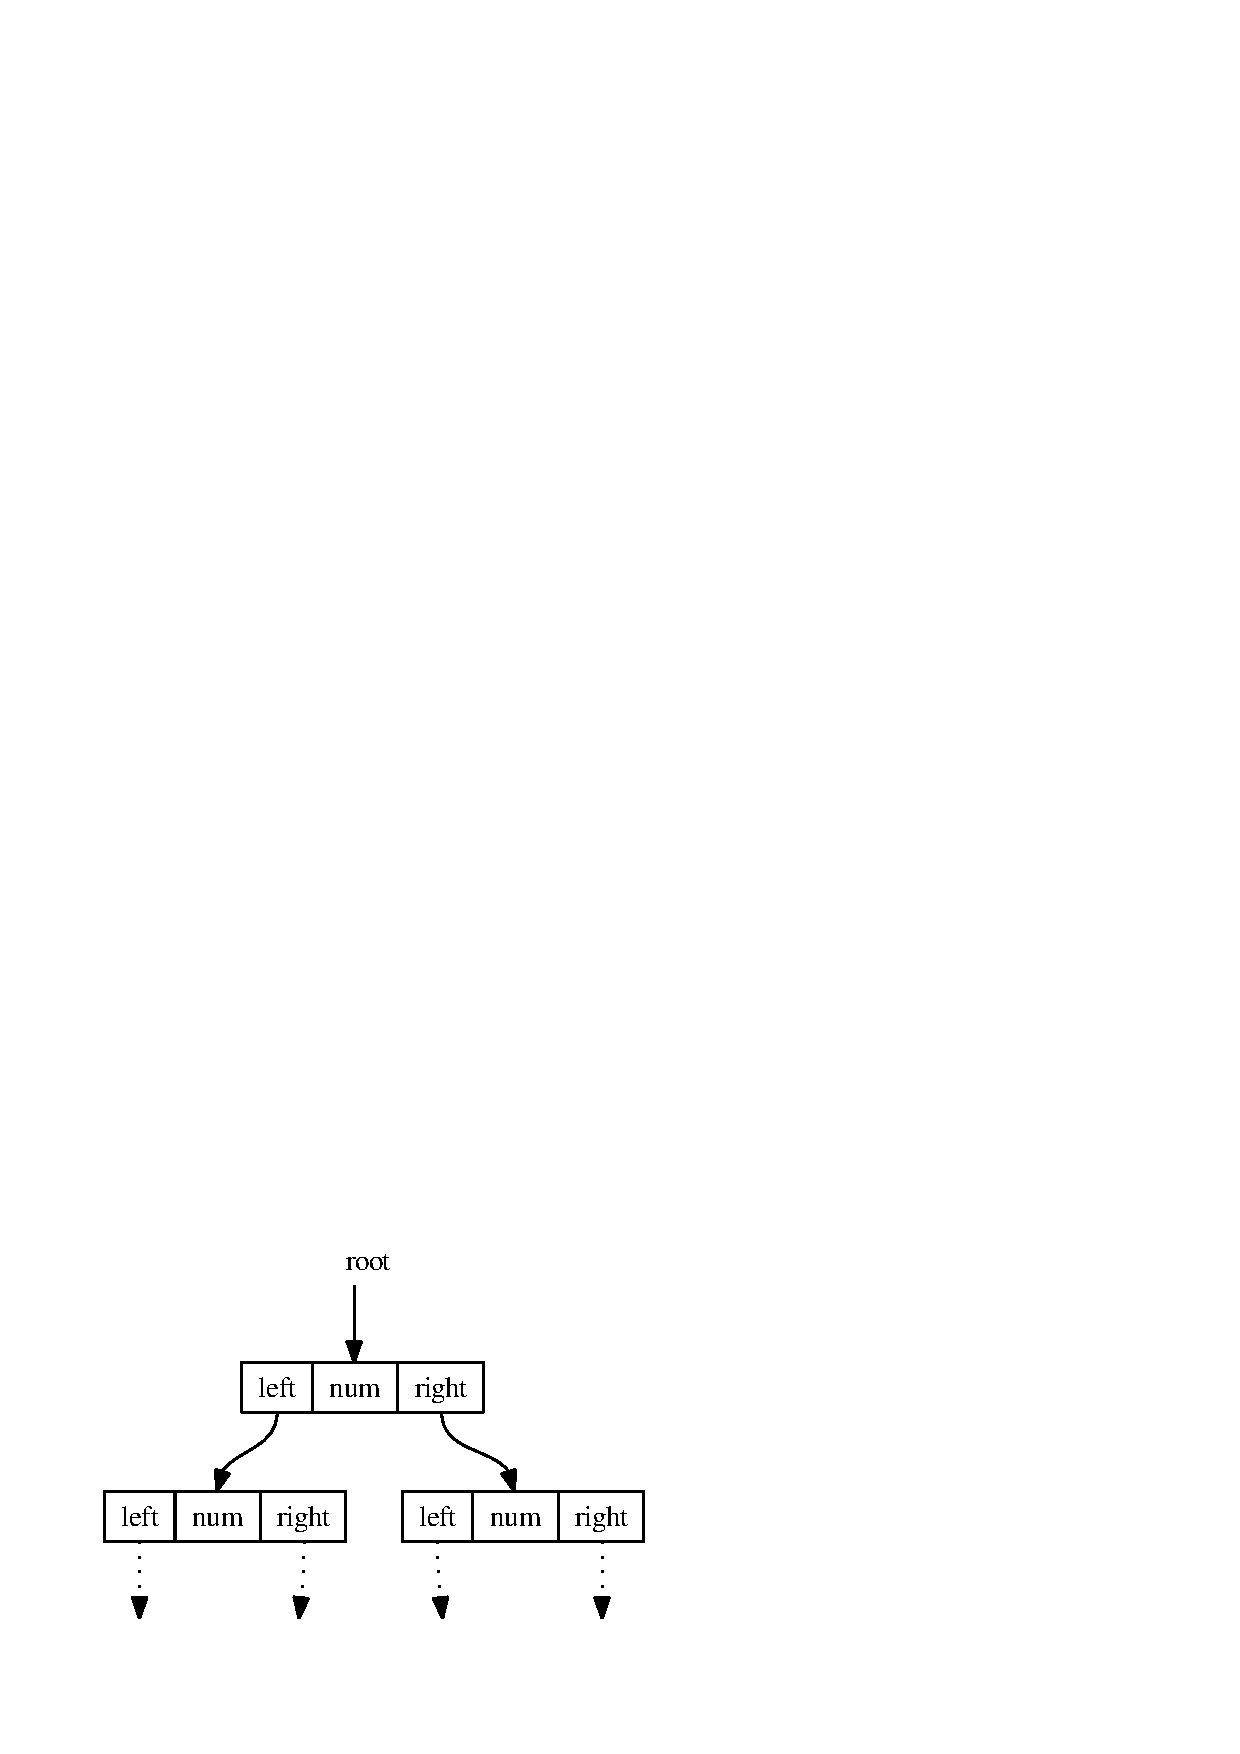
\includegraphics[scale=0.6]{tree_grph}
      & \\
%      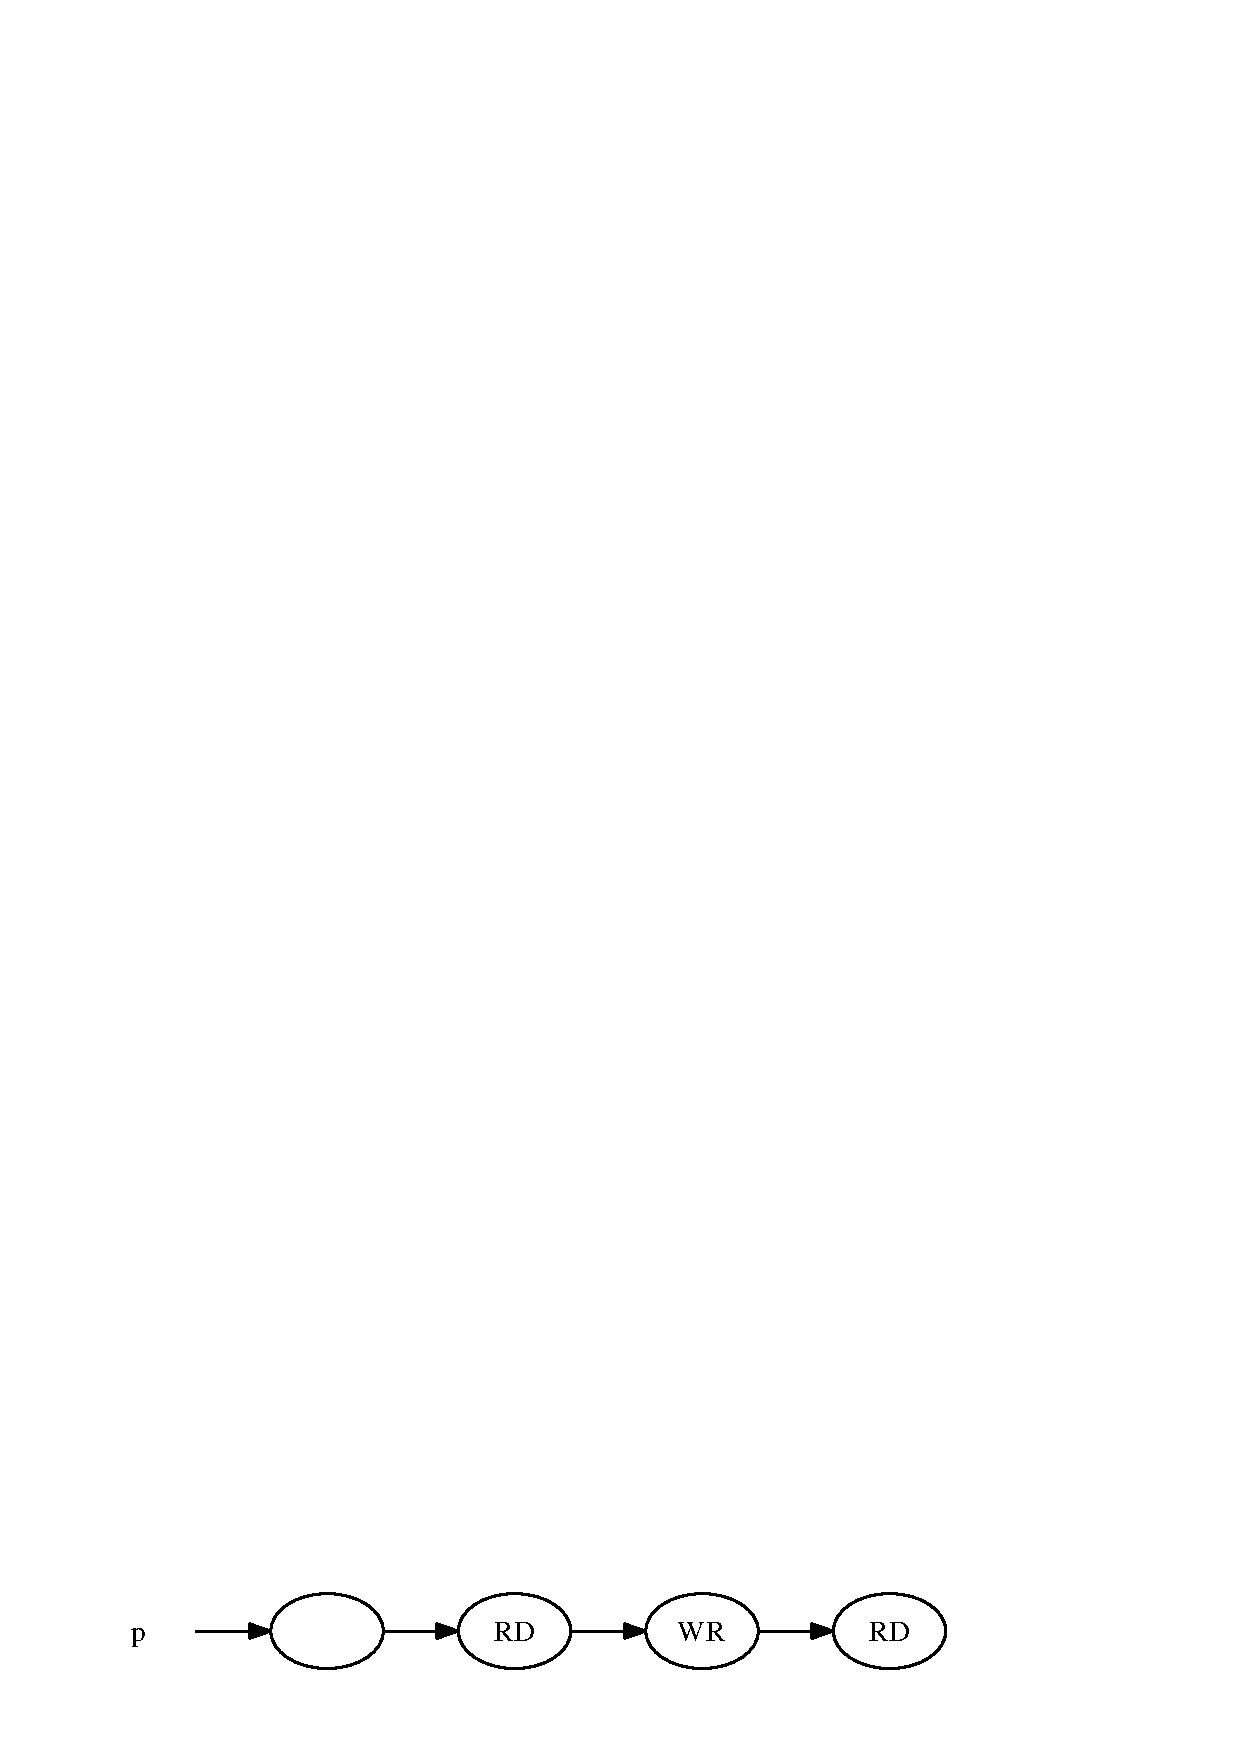
\includegraphics[scale=0.6]{grph_motiv} & \\
%      (a) & (b) \\
     (a) Data structure & 
     (b) Function traversing the data structure. \\
%    \hline 
    \end{tabular}}
  \end{center}
  \hrule
  \caption{\label{fig:motiv1} Motivating example: function-call parallelization}
%\hrule
\end{figure}
\begin{example}{\rm 
Consider Figure~\ref{fig:motiv1} which gives a motivational 
example for parallelism in the context of function calls. It shows 
the tree data 
structure and the function \emph{treeAdd} traversing on the 
data structure. In the code fragment the two calls to the function 
\emph{treeAdd} respectively perform the additions of left and right 
subtrees recursively. If the analysis can ensure that the two function calls 
do not access any common region of heap, they can be executed in parallel.
} 
\hfill\psframebox{}  
\end{example}
%%%%%%%%%%%%%%%%%
\begin{figure}[t]
  \begin{center}
  
    \scalebox{.85}{\begin{tabular}{ c | c }
 %   \hline
      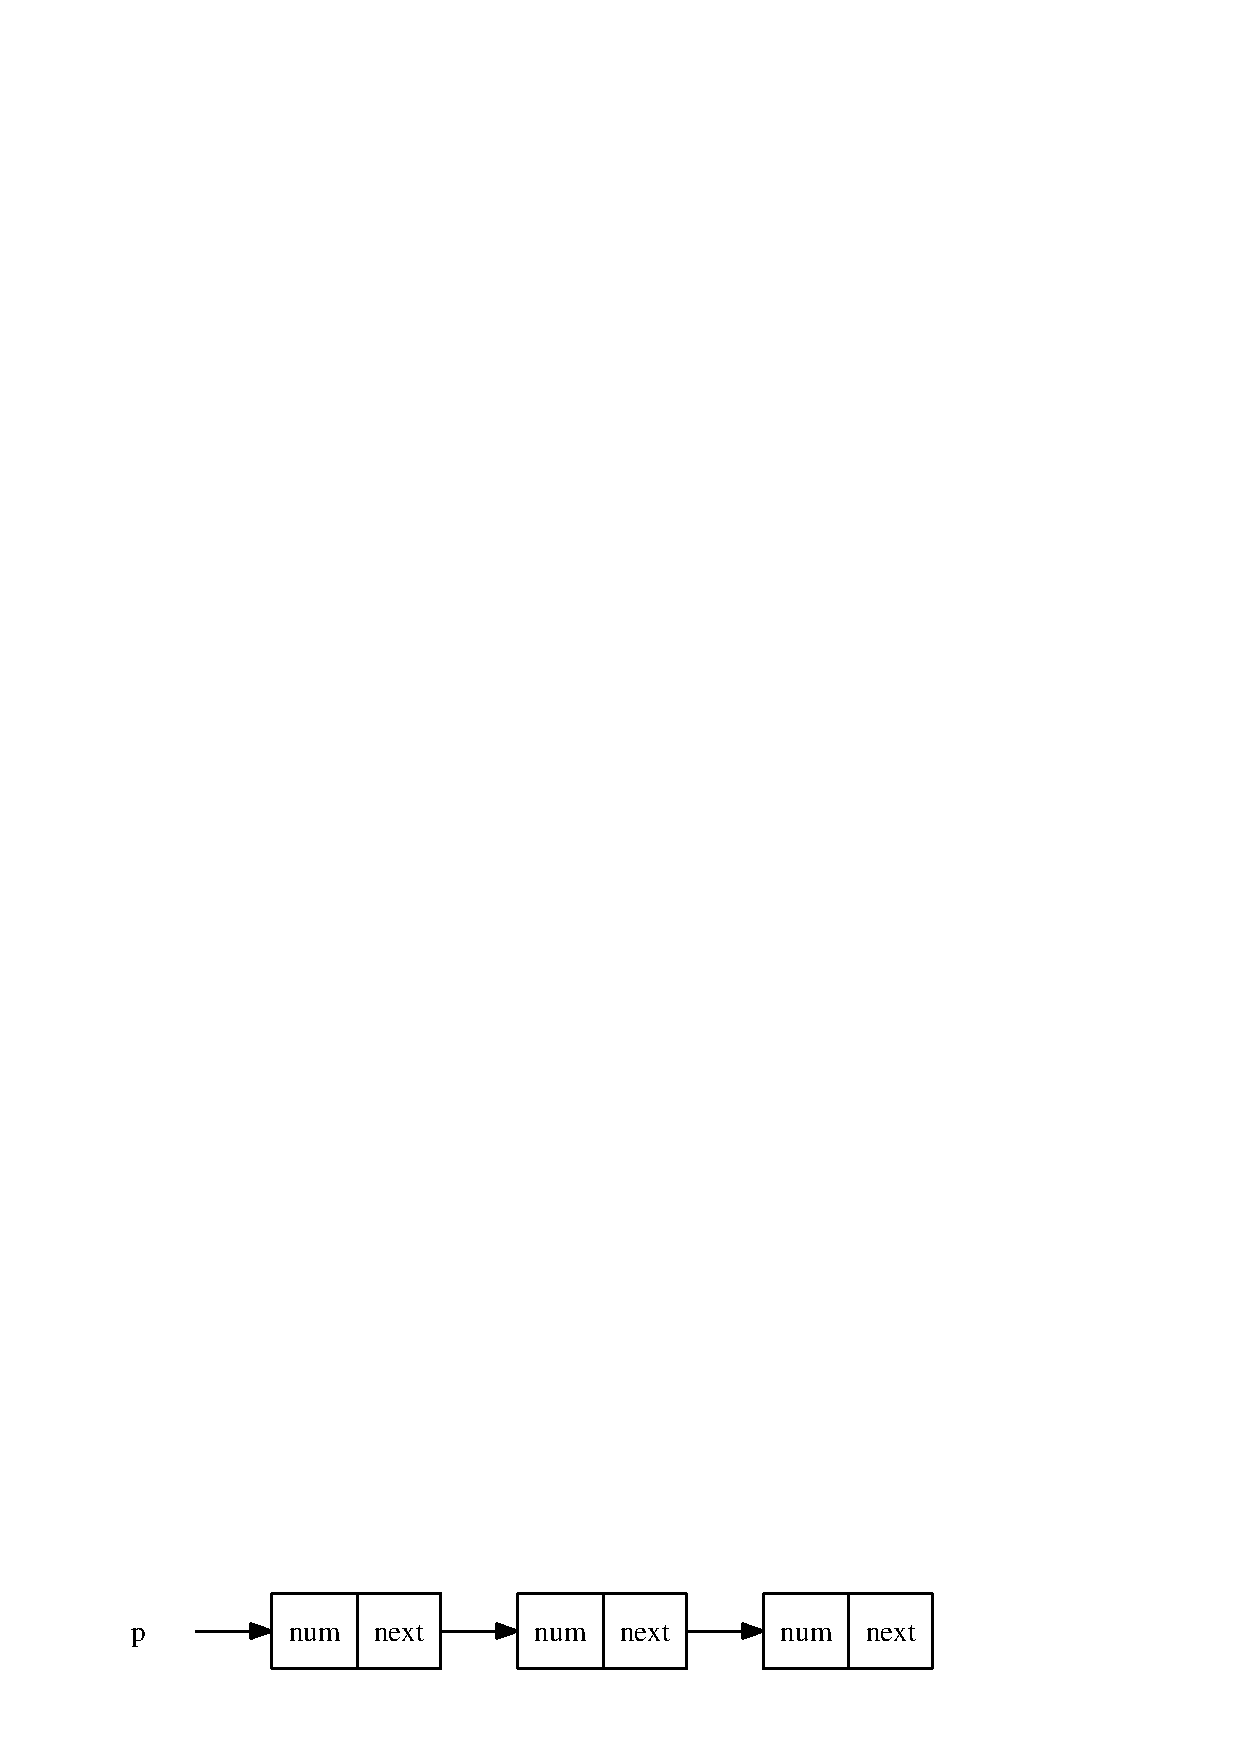
\includegraphics[scale=0.6]{grph4} %\cline{1-1}
      &
      {\tt
\begin{program}{0}
  \FL\ \ldots
  \NL{0} p = list;
  \UNL{0} \WHILE (p$\rightarrow$next != NULL) \{
  \NL{1}     q = p$\rightarrow$next;
  \NL{1}     temp = q$\rightarrow$num;
  \NL{1}     r = q$\rightarrow$next;
  \NL{1}     r$\rightarrow$num = temp;
  \NL{1}     p = r;
  \UNL{0} \}
  \UNL{0} \ldots
\end{program}
} \\
      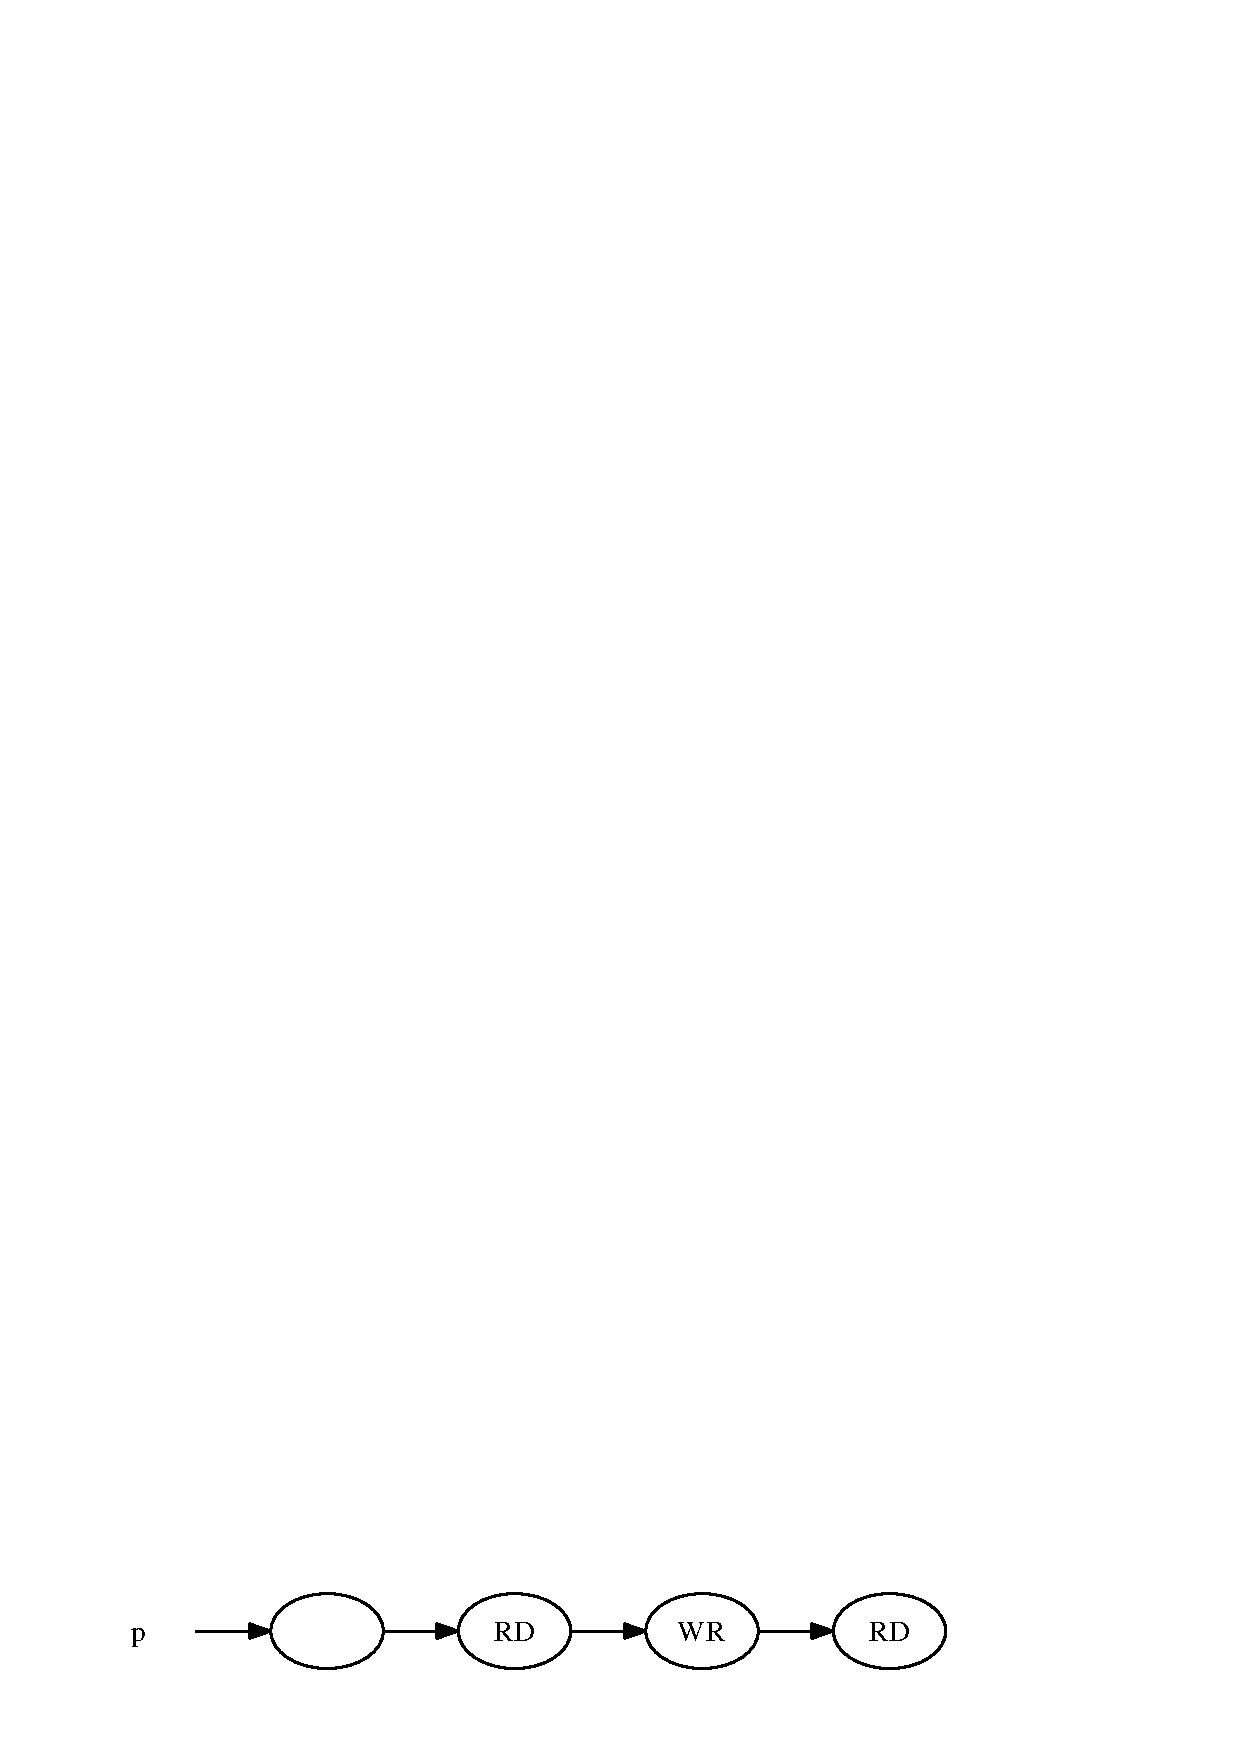
\includegraphics[scale=0.6]{grph_motiv} & \\
%      (a) & (b) \\
     (a) Nodes read and written by code & 
     (b) Loop traversing the data structure. \\
    \end{tabular}}
  \end{center}
  \hrule
  \caption{\label{fig:motiv} Motivating example: loop parallelization}
%\hrule
\end{figure}
\begin{example}{\rm
  Figure~\ref{fig:motiv}
  shows an example of loop level parallelism. It shows list data structure and the nodes of the structure being read and written, tagged by \emph{Read} (\ttf{RD}) 
  and \emph{Write} (\ttf{WR}) access by the code fragment traversing the
  data structure. Note that, the first node of the structure is a special node which is neither 
  read nor written by the code fragment. The performance of the code can be improved if the loop can
  be executed in parallel. However, without the knowledge of
  precise heap dependences, we have to assume worst case
  scenario, i.e.,  the  location read by the statement {\tt
    S3} in some iteration could be the same as the location
  written by the statement {\tt S5} in some other iteration.
  In that case,  it is not possible to parallelize the loop.
 
  Our dependence analysis can show that the locations read by
  {\tt S3} and those written by {\tt S5} are mutually
  exclusive. Further, it also shows the absence of any other
  dependences.  This information, along with the information
  from classical control and data dependence analysis, can be
  used by a parallelizing compiler to parallelize the loop.
}
\hfill\psframebox{}  
\end{example}

This report explains our approach for a practical heap data dependence analysis. 
As it is understood that we are only talking about data dependences, we drop the term 
data in the rest of the report. 
%
\section{Contributions of our Work}
Our work contributes in the area of heap based 
dependence analysis. We present a novel approach 
which identifies dependences and extracts parallelism for a sequential program. 
In particular, our approach finds out dependences between two statements. 
This enables us to find out whether two procedure calls 
access disjoint structures, hence can be executed in parallel. 
Then we refine this technique to work better 
in presence of loops. We also extend the work of loop analysis 
for static and scalar data to support heap intensive loops.

\section{Organization of the Thesis}
The rest of the thesis is organised as follows. We discuss about related 
work done in the field of heap intensive dependence analysis in Chapter~\ref{ch:RelatedWork}.
Chapter~\ref{ch:back} specifies the imperative programming model 
for which our analysis is defined and gives the other background 
details. Chapter~\ref{ch:dep} through~\ref{ch:interdep} provide a complete 
description of our practical dependence analysis applied to 
dynamically allocated structure. Chapter~\ref{ch:dep} gives the detailed 
explanation of the intra-procedural dependence detection technique 
which separately works on each procedure of a program. Chapter~\ref{ch:loopdep} 
presents our method to handle loops in a more specific way. We also 
give the inter-procedural framework for our analysis in Chapter~\ref{ch:interdep}. 
Chapter~\ref{ch:result} demonstrates our whole method by extensively 
analysing few benchmark codes. We conclude the report in Chapter~\ref{ch:conclusion} 
by giving the direction for future research.
% 
% 
\chapter{Background \label{Background}}
\section{Related Work}
It was for functional languages that first shape analysis was looked at. Jones and Muchnick~\cite{Muchnick79} 
suggested a method for finding shape of unbounded data objects in LISP like
languages using regular tree grammars. They associate with each program point a set of 
shape graphs and to handle termination of analysis they use k-limiting approach. So they treat all nodes
whose distance is more than k from root as a single summarized node. Due to its large consumption of space 
and time the analysis is not practical.

Chase et al.~\cite{Chase90}  has used the concept of heap reference counts. They associate each node with a reference 
count and then try to find that part of the heap where all nodes
have reference count as one, such portions are said to be a tree or list. 
They have tried to tackle the problems with k-limiting to some extent, however their work fails obtaining 
accurate results for recursive data structures.

Sagiv et al.~\cite{Sagiv99},~\cite{Sagiv02} have presented a family of abstract interpretation algorithms based on three-valued logic. 
They use abstraction, a method for summarizing node and to handle destructive updates they have 
come up with re-materialization which refers to the process of splitting summary nodes. An exponential number of shape nodes may arise because of
abstract interpretation, so its not suitable for practical purposes. Sagiv and Noam~\cite{SagivInter02} have also looked into inter procedural shape 
analysis for recursive programs but they work only on linked lists. 

The main idea of Brian et al.~\cite{hackett05region} is to  decompose heap abstractions and independently analyze different parts of the heap.
They also decompose memory abstraction horizontally and vertically. Now for the local work to propagate globally they proposed 
and used a context sensitive inter procedural shape analysis algorithm.

A dynamic shape analysis technique was proposed by Jump et al.~\cite{maria09dynamic}. They compute a class field 
summary graph that summarizes the dynamic object graph. This summary graph also records the in-degree and out-degree of each 
object which are the recursive degree metrics. In their analysis they keep track of those node which are of fixed degree and
also those whose degree is in a particular range. Since running the analysis after each pointer statement is very costly they 
do it by piggybacking with garbage collection. 

Susan et al.~\cite{sagivDemand95} have a polynomial worst case method for inter procedural analysis provided its a demand 
data flow analysis. It will determine whether a single given data flow value holds at some give point. But the class of problems 
it can handle was limited. Alexy~\cite{interAbstr06} represent heap portions independently by using the notions of abstraction and separation logic.
Their representation helps to easily separate the portion which is reachable and which is not from a procedure. Its limitation is that it 
supports only linked lists, doubly linked lists and trees.

Ghiya et al.~\cite{Ghiya96} estimates the shapes of heap structures pointed to by pointers as a \emph{Tree}, \emph{Dag} or \emph{Cycle}. 
They use Direction, Interference matrices and shape attributes as their data flow values which gets generated and killed after each pointer 
statements. As this is very closely related to our work, we have given a detailed view of it in the Appendix section.

Marron et al.~\cite{marron06static} uses a graph based heap model with objects being vertices and pointers being the labeled edges. 
A node is considered as a set of cells and each node is associated with a layout saying \emph{Singleton}, \emph{List}, \emph{Tree}, 
\emph{Multipath} or \emph{Cycle}. These layouts honors the order \emph{Singleton} $<$ \emph{List} $<$ \emph{Tree} $<$ \emph{Multipath} $<$ \emph{Cycle}. 
This means that suppose a node is of layout \emph{Tree} then it may have properties of \emph{Singleton}, \emph{List} or \emph{Tree}.
They have methods by which summarized nodes are split to concrete nodes (and edges) but its only for for the most common cases encountered, 
this enables them to handle strong updates. Then they have proposed a context sensitive analysis~\cite{marron08context} for the same graph based
heap models. For this they have come up with operations \emph{project}$/$\emph{extend}. \emph{project} removes that part of heap which is 
unaffected by a called procedure and \emph{extend} rejoins the unreachable portion back after return. 

The work of Sandeep et al.~\cite{Sandeep11thesis}, which is extended in the present paper, is explained in detail in the
following section for a better understanding of the basis of this work.

\section[Precise Shape Analysis using Field Sensitivity]{Analysis of Sandeep et. al.~\cite{Sandeep11thesis}\footnote{The contents of this section are borrowed from~\cite{Sandeep11thesis}}}
Most of the definitions and technical terms used in this section are borrowed from the aforementioned paper.
As we will be using these details so throughout the report we have mentioned this as a separate section in our report.
They have presented a shape analysis technique that uses limited field sensitivity to infer the shape. 
As this technique is able to handle destructive updates, so precise shape information can be obtained.
They generated data flow values in the form of field sensitive matrices and boolean equations at each program point to obtain the shape information.

\subsection{Definitions And Notations}
At a particular program point, the heap structure is viewed as a directed
graph, the nodes of which represent the allocated objects and
the edges represent the connectivity through pointer fields.
Pictorially, inside a node all the relevant pointer
variables are shown that can point to the heap object corresponding to
that node. The edges are labeled by the name of the
corresponding pointer field. 

Let $\heap$ denotes the set of all heap directed
pointers at a particular program point and $\fields$
denotes the set of all pointer fields at that program point.
Given two heap-directed pointers $\p$, $\q$ $\in$
$\heap$, a path from $\p$ to $\q$ is the sequence
of pointer fields that need to be traversed in the heap to
reach from $\p$ to $\q$.  The length of a path is
defined as the number of pointer fields in the path.  As the
path length between two heap objects may be unbounded, only the first field of a path is stored. 
To distinguish between a path of length one
(direct path) from a path of length greater than one
(indirect path) that start at the same field, the
superscript $\drct$ for a direct path and $\indrct$ for an
indirect path are used. In pictures, solid edges are used for direct
paths, and dotted edges for indirect paths.

It is also possible to have multiple paths between two
pointers starting at a given field $f$, with at most one
direct path $f^\drct$. However, the number of indirect paths
$f^\indrct$ may be unbounded. As there can only be a finite
number of first fields, first fields of paths are stored,
including the count for the indirect paths, between two
pointer variables in a set. To bound the size of the set, a limit $k$ is put 
on number of repetitions of a particular field. If the number goes beyond $k$, the number of
paths with that field is treated as $\infty$. 

\begin{example} {\rm
\begin{figure}
\centering
\newcommand{\smf}{$f$}%%\scriptstyle f$}
\newcommand{\smh}{$h$}%%\scriptstyle h$}
\newcommand{\smg}{$g$}%%\scriptstyle g$}
\begin{tabular}{@{}cc@{}}
{\small \tt
    \begin{tabular}[b]{l}
      S1. q = p; \\
      S2. {\bf while}(...) \{ \\
      S3. \ \ \ \ q$\rightarrow$g = s; \\
      S4. \ \ \ \ q = q$\rightarrow$f; \\
      S5. \} \\
    \end{tabular}
  } &
 \scalebox{0.8}{ \psset{unit=1mm}
  \begin{pspicture}(0,0)(50,30)
    %%\psframe(0,0)(50,30)
    \putnode{q0}{origin}{3}{3}{}
    \putnode{q1}{q0}{0}{0}{\pscirclebox{\mbox{\p}}}
    \putnode{q2}{q1}{10}{0}{\pscirclebox[framesep=2.5]{\mbox{}}}
    \putnode{q3}{q2}{10}{0}{\mbox{\ldots}}
    \putnode{q4}{q3}{10}{0}{\pscirclebox{\mbox{\q}}}
    \putnode{q5}{q4}{10}{0}{\pscirclebox[framesep=2.5]{\mbox{}}}
    
    \ncline{->}{q1}{q2}
    \Bput[0.2]{\smf}
    \ncline{->}{q2}{q3}
    \Bput[0.2]{\smf}
    \ncline{->}{q3}{q4}
    \Bput[0.2]{\smf}
    \ncline{->}{q4}{q5}
    \Bput[0.2]{\smf}
    
    \putnode{s0}{q4}{15}{15}{\pscirclebox{\mbox{\s}}}
    \nccurve[angleA=90,angleB=145,ncurv=1]{->}{q1}{s0}
    \Aput[.1]{\smg}
    
    \putnode{t0}{q2}{0}{15}{\pscirclebox[framesep=2.5]{\mbox{}}}
    \nccurve[linestyle=dotted, dotsep=.5, angleA=-55,angleB=-165,
      ncurv=.2,nodesepA=-.3]{->}{t0}{s0}
    
    \ncline[linestyle=dotted, dotsep=.5]{->}{t0}{s0}
    \nccurve[linestyle=dotted, dotsep=.5,angleA=55,angleB=165,
      ncurv=.3,nodesepA=-.3]{->}{t0}{s0}
    

    \ncline[nodesepA=-.5,nodesepB=-.5]{->}{q1}{t0}
    \Aput[.1]{\smh}
    
    \ncline{->}{q2}{s0}
    \Bput[0.2]{\smg}
    \ncline[nodesepA=-.75,nodesepB=-.75]{->}{q4}{s0}
    \Bput[0.2]{\smg}
\end{pspicture}} \\
\scalebox{0.80}{ (a) A code fragment} & \scalebox{0.80}{ (b) 
  \begin{tabular}[t]{@{}p{95mm}}
    A possible heap graph for code in (a). Solid edges are the
    direct paths, dotted edges are the indirect paths.
  \end{tabular}}
  \end{tabular}
\caption{Paths in a heap graph}
\label{fig:pathsAndSets}
\end{figure}


Figure~\ref{fig:pathsAndSets}(a) shows a code fragment and
Fig.~\ref{fig:pathsAndSets}(b) shows a possible heap graph
at a program point after line {\tt S5}. In any execution, there is one path
between $\p$ and $\q$, starting with field $f$, whose
length is statically unknown. This information is stored by
as the set $\{\fieldI{f}{}{1}\}$. Further, there are
unbounded number of paths between $\p$ and $\s$, all
starting with field $f$. There is also a direct path from
$\p$ to $\s$ using field $g$, and 3 paths starting with
field $h$ between $\p$ and $\s$. Assuming the limit $k
\geq 3$, this information can be represented by the set $\{
g^\drct, f^{\indrct\infty}, h^{\indrct 3} \}$. On the other hand, if $k < 3$,
then the set would be $\{ g^\drct, f^{\indrct\infty}, h^{\indrct\infty} \}$.
  } \hfill\psframebox{}
\end{example}

For brevity, 
$f^{\anysup}$ is used for the cases when it is irrelevant to
distinguish between direct or indirect path starting at the
first field $f$. Next field sensitive matrices are defined.

%FIELD SENSITIVE DIRECTION MATRIX 
\begin{definition}
\label{DFM_matrix}
Field sensitive Direction matrix
$D_F$ is a matrix that stores information 
about paths between two pointer variables.
Given $\p, \q \in
\heap, f \in \fields$:
\begin{eqnarray*}
  \epsilon & \in \DFM{p}{p}& \mbox{ where $\epsilon$
    denotes the empty path.} \\
  f^\drct  &\in  \DFM{p}{q} & \mbox{ if there is a direct
    path $f$ from $\p$ to $\q$.}\\
  f^{\indrct m} & \in  \DFM{p}{q} & 
  \mbox{\begin{tabular}[t]{p{105mm}}if there are $m$ indirect
      paths starting with field $f$ from $\p$ to $\q$ and $m
      \leq k.$
    \end{tabular}
  } \\
  f^{\indrct\infty} & \in  \DFM{p}{q} &
  \mbox{\begin{tabular}[t]{p{105mm}}if there are $m$ indirect
      paths starting with field $f$ from $\p$ to $\q$ and $m >
      k.$
  \end{tabular}}  
\end{eqnarray*}
\end{definition}

Let \nat\ denote the set of natural numbers. The
following partial order are defined for approximate paths used by the
analysis. For $ f \in \fields,\ m,n \in \nat,\ n \leq m$:
$$
\epsilon \sqsubseteq \epsilon, \quad 
f^\drct \sqsubseteq  f^\drct,  \quad
f^{\indrct\infty}  \sqsubseteq  f^{\indrct\infty}, \quad
f^{\indrct m} \sqsubseteq f^{\indrct\infty}, \quad
f^{\indrct n} \sqsubseteq f^{\indrct m} \enspace .
$$
The partial order is extended to set of paths $S_{P_1},
S_{P_2}$ as\footnote{Note that for the analysis, for a given
  field $f$, these sets contain at most one entry of type
  $f^\drct$ and at most one entry of type $f^\indrct$}:
\begin{eqnarray*}
  S_{P_1} \sqsubseteq S_{P_2} &\Leftrightarrow& \forall \alpha \in
  S_{P_1}, \exists \beta \in S_{P_2}\ s.t. \alpha \sqsubseteq \beta \enspace .
\end{eqnarray*}
For pair of paths:
\begin{eqnarray*}
  (\alpha, \beta) \sqsubseteq (\alpha', \beta') 
  \Leftrightarrow 
   (\alpha \sqsubseteq \alpha')  \wedge
  (\beta \sqsubseteq  \beta')
\end{eqnarray*}
For set of pairs of paths $R_{P_1}, R_{P_2}$:
\begin{eqnarray*}
  R_{P_1} \sqsubseteq R_{P_2} \Leftrightarrow \forall
  (\alpha, \beta) \in
  R_{P_1}, \exists (\alpha', \beta') \in
  R_{P_2}\ s.t. (\alpha, \beta) \sqsubseteq (\alpha', \beta')
\end{eqnarray*}


Two pointers $\p,\q \in \heap$ are said to
interfere if there exists $\s \in \heap$ such that both
$\p$ and $\q$ have paths reaching $\s$. Note that $\s$ could
be $\p$ (or $\q$) itself, in which case the path from $\p$
(from $\q$) is $\epsilon$.

%FIELD SENSITIVE DIRECTION MATRIX 
\begin{definition}\label{IFM_matrix}
Field sensitive Interference matrix $I_F$ between
two pointers captures the ways in which these pointers are
interfering.  For $\p, \q, \s \in \heap, \p \not= \q$,
the following relation holds for $D_F$ and $I_F$: 
\begin{eqnarray*}
  \DFM{p}{s} \times \DFM{q}{s} &\sqsubseteq&
  \IFM{p}{q} \enspace . \label {eq:rel-df-if}
\end{eqnarray*}
\end{definition}

The analysis computes over-approximations for the matrices
$D_F$ and $I_F$ at each program point. While it is possible
to compute only $D_F$ and use above equation to
compute $I_F$, computing both explicitly results in better
approximations for $I_F$. Note that interference relation is
symmetric, i.e.,
\begin{eqnarray*}
  (\alpha, \beta) \in I_F[\p, \q] \Leftrightarrow
   (\beta, \alpha) \in I_F[\q, \p] \enspace .
\end{eqnarray*}
While describing the analysis, the
above relation is used to show the computation of only one of the two
entries. 

\begin{figure}
\centering
\begin{tabular}{c@{$\qquad\qquad$}c}
\psset{unit=1.2mm}
\begin{pspicture}(0,0)(15,20)
	\psset{linecolor=black}
  \putnode{p0}{origin}{3}{9}{\pscirclebox{\p}}
  \putnode{q0}{p0}{5}{7}{\pscirclebox{\q}}
  %\putnode{r0}{p0}{0}{-14}{\pscirclebox{\myr}}
  \putnode{r0}{p0}{10}{0}{\pscirclebox{\myr}}
	\psset{linecolor=black}
  \ncline[nodesep=-.3]{<-}{p0}{q0}
  \aput[0.2](0.4){$\scriptstyle f$}
  \ncline{<-}{p0}{r0}
  \aput[0.2](0.4){$\scriptstyle g$}
%   %\ncline[nodesep=-.5]{->}{s0}{r0}
%   %\aput[0.2](0.2){$\scriptstyle f_5$}
%   \nccurve[angleA=45,angleB=0,linestyle=dotted,dotsep=0.2,ncurv=1,nodesepA=-.8]{->}{p0}{s0}
%   \aput[0.2](0.2){$\scriptstyle f_2$}
%   %\nccurve[angleA=180,angleB=225,linestyle=dotted,dotsep=0.2,ncurv=1,nodesepB=-.5]{->}{q0}{r0}
%   %\bput[0.2](0.2){$\scriptstyle f_4$}
\end{pspicture} &
\scalebox{0.8}{
\renewcommand{\arraystretch}{1.2}
\begin{tabular}[b]{|c|c|c|c|}
\hline
$D_F$          & \p                          & \q                             &  \myr  \\ \hline \hline 
\p 	           & $\{\epsilon\}$              & $\emptyset$            & $\emptyset$     \\ \hline 
\q             & $\{\fieldD{f}{}\}$                  & $\{\epsilon\}$                 & $\emptyset$   \\ \hline
\myr             & $\{\fieldD{g}{}\}$                 & $\emptyset$                    & $\{\epsilon\}$       \\ \hline
\end{tabular}} \\
\scalebox{0.80}{ (a) Heap graph} & \scalebox{0.80}{ (b) Direction Matrix}  \\ \\
% \multicolumn{2}{c}{
& \multirow{6}{*}{
\begin{tabular}{c}
$f_{\q\p} = \true$ \\
$f_{\p\q} = \false$ \\
$g_{\myr\p} = \true$ \\ 
\end{tabular}
} \\

\scalebox{0.80}{
\renewcommand{\arraystretch}{1.2}
\newcommand{\iwd}{0.23\columnwidth}
\begin{tabular}[b]{|c|c|c|c|}
\hline 
$\ I_F$     & $\p$	               & $\q$ &  $\myr$             \\ \hline \hline 
%%
$\p$ & $\{\epsilon, \epsilon\}$    & $\{(\epsilon, \fieldD{f}{}) \}$               & $\{(\epsilon, \fieldD{g}{})\}$      \\      \hline 
%%
$\q$       & $\{(\fieldD{f}{}, \epsilon)\}$                 & $\{\epsilon, \epsilon\}$          & $\{(\fieldD{f}{}, \fieldD{g}{})\}$         \\  \hline              
%%
$\myr$       & $\{(\fieldD{g}{}, \epsilon)\}$             & $\{(\fieldD{g}{}, \fieldD{f}{})\}$             & $\{\epsilon, \epsilon\}$         \\ \hline              
%%
\end{tabular}} &  \\
% } \\
% \multicolumn{2}{c}{\scalebox{0.80}{ (c) Interference Matrix} }
\scalebox{0.80}{(c) Interference Matrix}  & \scalebox{0.80}{(d) Bolean variables}
\end{tabular}
%\caption{A heap graph and its field sensitive path matrices\label{fig:DFM_IFM}}
\end{figure}


\begin{example}{\rm
Figure~\ref{fig:DFM_IFM} shows a heap graph and the
corresponding field sensitive matrices as computed by the
analysis.  } \hfill\psframebox{}
\end{example}

As mentioned earlier, for each variable $\p \in \heap$, the
analysis uses attributes $\p_{\subD}$ and $\p_{\subC}$ to
store boolean functions telling whether $\p$ can reach a DAG or
cycle respectively in the heap. The boolean functions
consist of the values from matrices $D_F$, $I_F$, and the field
connectivity information. For $f \in \fields, \p, \q \in
\heap$, field connectivity is captured by boolean variables
of the form $f_{pq}$, which is true when $f$ field of $\p$ points
directly to $\q$. 
The shape of \p, \p.\shape, can be obtained by evaluating
the functions for the attributes $\p_{\subC}$ and
$\p_{\subD}$, and using Table~\ref{tbl:det_shape}.
\begin{table}
\caption{Determining shape from boolean
  attributes\label{tbl:det_shape}}
\begin{center}
\begin{tabular*}{0.75\textwidth}{@{\extracolsep{\fill}} cccc|c }
\hline
$\p_{\subC}$ &$\quad$ & $\p_{\subD}$ &$\quad$& $\p.\shape$ \\ 
\hline
\true  && Don't Care  && Cycle        \\ 
\false  && \true          && DAG    \\ 
\false  && \false          && Tree   \\ 
\hline
\end{tabular*}
\end{center}
\end{table}

The following operations are used in the analysis. Let $S$
denote the set of approximate paths between two nodes, $P$
denote a set of pair of paths, and $k \in \nat$ denotes the
limit on maximum indirect paths stored for a given
field. Then,
\begin{itemize}
\item Projection: For $f \in \fields$,
  \project{S}{f}\ extracts the paths starting at field $f$.
  $$\project{S}{f} \equiv S \cap \{f^{\drct}, f^{\indrct 1}, \ldots,
  f^{\indrct k}, f^{\indrct \infty}\} \enspace .$$

\item Counting: The count on the number of paths is defined
  as :
  \begin{eqnarray*}
   \num{\epsilon} =     1, \qquad
   \num{f^{\drct}} =     1, &\qquad&
   \num{f^{\indrct\infty}} =     \infty, \qquad
   \num{f^{\indrct j}} =  j \mbox{ for } j \in \nat \\
   \num{S} &=&   \sum_{\alpha \in S}\num{\alpha} 
  \end{eqnarray*}

Also,  
  \begin{eqnarray*}
   \num{(\alpha, f^{\indrct m})} &=&  \left\{ \begin{array}{@{}ll}  
   			m        &  \mbox{if } \alpha \in \{f^{\drct}, \epsilon\} \\
			m*n      &  \mbox{if } \alpha = f^{\indrct n} \\
			\infty   &  \mbox{if } \alpha = f^{\indrct\infty} \\
			\end{array}\right. \\
   \num{(f^{\indrct m}, \beta)} &=&  \left\{ \begin{array}{@{}ll}  
   			m        &  \mbox{if } \beta \in \{f^{\drct}, \epsilon\} \\
			m*n      &  \mbox{if } \beta = f^{\indrct n} \\
			\infty   &  \mbox{if } \beta = f^{\indrct\infty} \\
			\end{array}\right. \\
   \num{(\alpha, \beta)} &=&  \begin{array}{@{}ll}
   			 1       &  \mbox{if } \alpha, \beta \in \{f^{\drct}, \epsilon\} \\
			\end{array} \\
   \num{(f^{\indrct\infty}, \beta)} &=&  \begin{array}{@{}ll}
   			 \infty       &  \mbox{where }  \beta \in \{f^{\drct}, \epsilon, f^{\indrct\infty}\} \\
			\end{array} \\
   \num{(\alpha, f^{\indrct\infty})} &=&  \begin{array}{@{}ll}
   			 \infty       &  \mbox{where } \alpha \in \{f^{\drct}, \epsilon, f^{\indrct\infty}\} \\
			\end{array} \\
	\num{P} &=&   \sum_{(\alpha, \beta) \in P}\num{(\alpha, \beta)}		
  \end{eqnarray*}

\item Path removal, intersection and union over set of
  approximate paths : For singleton sets of paths
    $\{\alpha\}$ and $\{\beta\}$, path removal
    (\remOne{\{\alpha\}}{\{\beta\}}), intersection
    ($\{\alpha\} \cap \{\beta\}$) and union($\{\alpha\} \cup
    \{\beta\}$) operations are defined as given in
    Table~\ref{tab:path-ops}. These definitions can be extended
    to set of paths in a natural way. For example,
	for general sets of paths, $S_1$ and $S_2$, 
	the definition of removal can be extended as:
\begin{eqnarray*}
  \remOne{S_1}{S_2}  = \bigcap_{\beta \in
    {S_2}}(\bigcup_{\alpha \in {S_1}}  \remOne{\{\alpha\}}{\{\beta\}}  )
\end{eqnarray*}

\begin{table}[t]
\caption{Path removal, intersection and union
  operations, where $\gamma$ denotes any other path.\label{tab:path-ops}}
\begin{center}
\scalebox{0.8}{
\renewcommand{\arraystretch}{1.1}
\begin{tabular}{c@{$\qquad\qquad$}c}
(a) Path removal & (b) Intersection \\ 
%\begin{tabular*}{0.55\textwidth}{@{\extracolsep{\fill}} cc|ccccc}
\begin{tabular*}{0.55\textwidth}{@{}c@{}c@{}|ccccc}
  \hline
  $\remOne{}{}$ & $\{\beta\}$ & $\{\epsilon\}$ & $\{f^{\drct}\}$ & $\{f^{\indrct j}\}$& $\{f^{\indrct\infty}\}$ &  $\{\gamma\}$ \\
  $\{\alpha\}$ && & & & & 
  \\ \hline %\hline
  $\{\epsilon\}$ && $\emptyset$  & $\{\epsilon\}$ & $\{\epsilon\}$ & $\{\epsilon\}$ & $\{\epsilon\}$ \\ %\hline
  $\{f^{\drct}\}$ && $\{f^{\drct}\}$ & $\emptyset$ & $\{f^{\drct}\}$ & $\{f^{\drct}\}$ & $\{f^{\drct}\}$ \\ %\hline
  $\{f^{\indrct i}\}$ && $\{f^{\indrct i}\}$ & $\emptyset$ & $\{f^{\indrct m}\}$& $\emptyset$ & $\{f^{\indrct i}\}$ \\ %\hline
  $\{f^{\indrct\infty}\}$ && $\{f^{\indrct\infty}\}$ &$\emptyset$ & $\{f^{\indrct \infty}\}$& $\{f^{\indrct
    \infty}\}$ & $\{f^{\indrct\infty}\}$ \\ \hline
\end{tabular*} &
%\begin{tabular*}{0.50\textwidth}{@{\extracolsep{\fill}} cc|ccccc}
\begin{tabular*}{0.50\textwidth}{@{}c@{}c@{}|ccccc}
  \hline
  $\cap$&$\{\beta\} $& $\{\epsilon\}$ & $\{f^{\drct}\}$ &
  $\{f^{\indrct j}\}$& $\{f^{\indrct\infty}\}$ & $\{\gamma\}$ \\
  $\{\alpha\}$ && & & & & 
  \\ \hline %\hline
  $\{\epsilon\}$ && $\epsilon$  & $\emptyset$ & $\emptyset$ & $\emptyset$ & $\emptyset$ \\ %\hline
  $\{f^{\drct}\}$ && $\emptyset$ & $\{f^{\drct}\}$ & $\emptyset$ & $\emptyset$ & $\emptyset$ \\ %\hline
  $\{f^{\indrct i}\}$ && $\emptyset$ & $\emptyset$ & $\{f^{\indrct n}\}$& $\{f^{\indrct i}\}$ & $\emptyset$ \\ %\hline
  $\{f^{\indrct\infty}\}$ && $\emptyset$ &$\emptyset$ & $\{f^{\indrct j}\}$& $\{f^{\indrct \infty}\}$ & $\emptyset$ \\ \hline
\end{tabular*} \\
& \\
\multicolumn{2}{c}{(c) Union} \\
\multicolumn{2}{c}{
%\begin{tabular*}{0.75\textwidth}{@{\extracolsep{\fill}} cc|ccccc}
\begin{tabular*}{0.72\textwidth}{@{}c@{}c@{}|ccccc}
  \hline
  $\cup$&$\{\beta\} $& $\{\epsilon\}$ & $\{f^{\drct}\}$ &
  $\{f^{\indrct j}\}$& $\{f^{\indrct\infty}\}$ & $\{\gamma\}$ \\
  $\{\alpha\}$ && & & & &  
 \\ \hline %\hline
  $\{\epsilon\}$ && $\{\epsilon\}$  & $\{\epsilon, \fieldD{f}{}\}$ & $\{\epsilon, \fieldI{f}{}{j} \}$ & $\{\epsilon, \fieldI{f}{}{\infty}\}$ & $\{\epsilon, \gamma\}$  \\ %\hline
  $\{f^{\drct}\}$ && $\{\fieldD{f}{}, \epsilon\}$ & $\{\fieldD{f}{}\}$ & $\{\fieldD{f}{}, \fieldI{f}{}{j}\}$ & $\{\fieldD{f}{}, \fieldI{f}{}{\infty}\}$ & $\{\fieldD{f}{}, \gamma\}$  \\ %\hline
  $\{f^{\indrct i}\}$ && $\{\fieldI{f}{}{i}, \epsilon\}$ & $\{\fieldI{f}{}{i}, \fieldD{f}{}\}$ & $\{\fieldI{f}{}{t}\}$& $\{\fieldI{f}{}{\infty}\}$ & $\{\fieldI{f}{}{i}, \gamma\}$  \\ %\hline
  $\{f^{\indrct\infty}\}$ && $\{\fieldI{f}{}{\infty},
 \epsilon\}$ & $\{\fieldI{f}{}{\infty}, \fieldD{f}{}\}$ &
 $\{\fieldI{f}{}{\infty}\}$& $\{\fieldI{f}{}{\infty}\}$ &
 $\{\fieldI{f}{}{\infty}, \gamma\}$  \\ \hline
\end{tabular*}} \\& \\
\multicolumn{2}{c}{
 $i, j  \in \nat$, $m = {\tt max}(i-j, 0)$, $n = {\tt
  min}(i, j)$ and $t = \left\{\begin{array}{lcl}
  i+j    && \mbox { if } i+j \leq k \\
  \infty && \mbox{ Otherwise} 
  \end{array}\right.$.
}
\end{tabular}}
\end{center}
\end{table}


\item Path removal, intersection and union over set of pair
  of paths : For singleton sets of paths
    $\{\alpha, \beta\}$ and $\{\gamma, \delta\}$, union($\{\alpha, \beta\} \cup
    \{\gamma, \delta\}$), intersection
    ($\{\alpha, \beta\} \cap  \{\gamma, \delta\}$) and path removal
    (\remOne{\{\alpha, \beta\}}{\{\gamma, \delta\}}) operations are defined as given in
    Figure~\ref{tab:union_path_pair}, ~\ref{tab:intersection_path_pair} and ~\ref{tab:removal_path_pair} respectively. As before these 
	definitions can be extended to set of pair of paths in a natural way. For example,
	for general sets of paths, $P_1$ and $P_2$, 
	the definition of removal can be extended as:
\begin{eqnarray*}
  \remOne{P_1}{P_2}  = \bigcap_{(\gamma, \delta) \in
    {P_2}}(\bigcup_{(\alpha, \beta) \in {P_1}}  \remOne{\{\alpha, \beta\}}{\{\gamma, \delta\}}  )
\end{eqnarray*}

\begin{figure}
\caption{Union operation between two singleton sets of pair of paths, where $\{\alpha, \beta\}$ denote any other pair of paths and
$x$, $y$, $m$, $n$ can be any positive integer or $\infty$
\label{tab:union_path_pair}}
\begin{tabular}{c}
\\
\scalebox{0.65}{
\begin{tabular}{|c|c|c|c|c|c|}
\hline
$\cup$ & \{(\fieldD{f}{},\fieldD{g}{})\} & \{(\fieldI{f}{}{m},\fieldD{g}{})\} & \{(\fieldD{f}{},\fieldI{g}{}{n})\} & \{(\fieldI{f}{}{m},\fieldI{g}{}{n})\} & \{($\alpha$, $\beta$)\}\\ \hline

\{($\epsilon$,$\epsilon$)\} & \{($\epsilon$,$\epsilon$),(\fieldD{f}{},\fieldD{g}{}),  & \{($\epsilon$,$\epsilon$),(\fieldI{f}{}{m},\fieldD{g}{}),  & \{($\epsilon$,$\epsilon$),(\fieldD{f}{},\fieldI{g}{}{n}),  & \{($\epsilon$,$\epsilon$),(\fieldI{f}{}{m},\fieldI{g}{}{n}),  & \{($\epsilon$,$\epsilon$),\\
& ($\epsilon$,\fieldD{g}{}),(\fieldD{f}{},$\epsilon$ )\} & ($\epsilon$,\fieldD{g}{}),(\fieldI{f}{}{m},$\epsilon$ )\} & ($\epsilon$,\fieldI{g}{}{n}),(\fieldD{f}{},$\epsilon$ )\} & ($\epsilon$,\fieldI{g}{}{n}),(\fieldI{f}{}{m},$\epsilon$ )\} & ($\alpha$, $\beta$) \}\\ \hline

\{($\epsilon$,\fieldD{g}{})\} & \{($\epsilon$,\fieldD{g}{}),(\fieldD{f}{},\fieldD{g}{})\} & \{($\epsilon$,\fieldD{g}{}),(\fieldI{f}{}{m},\fieldD{g}{})\} & \{($\epsilon$,\fieldD{g}{}),(\fieldD{f}{},\fieldI{g}{}{n}),  & \{($\epsilon$,\fieldD{g}{}),(\fieldI{f}{}{m},\fieldI{g}{}{n}),  & \{($\epsilon$,\fieldD{g}{}), \\
& & & ($\epsilon$,\fieldI{g}{}{n}),(\fieldD{f}{},\fieldD{g}{})\} & ($\epsilon$,\fieldI{g}{}{n}),(\fieldI{f}{}{m},\fieldD{g}{})\} & ($\alpha$, $\beta$)\}\\ \hline

\{($\epsilon$,\fieldI{g}{}{y})\} & \{($\epsilon$,\fieldI{g}{}{y}),(\fieldD{f}{},\fieldD{g}{}) & \{($\epsilon$,\fieldI{g}{}{y}),(\fieldI{f}{}{m},\fieldD{g}{}) & \{($\epsilon$,\fieldI{g}{}{n+y}),(\fieldD{f}{},\fieldI{g}{}{n+y})\} & \{($\epsilon$,\fieldI{g}{}{n+y}),(\fieldI{f}{}{m},\fieldI{g}{}{n+y})\} & \{($\epsilon$,\fieldI{g}{}{y}), \\
& ($\epsilon$,\fieldD{g}{}),(\fieldD{f}{},\fieldI{g}{}{y})\} & ($\epsilon$,\fieldD{g}{}),(\fieldI{f}{}{m},\fieldI{g}{}{y})\} & & & ($\alpha$, $\beta$)\}\\ \hline

\{(\fieldD{f}{},$\epsilon$)\} & \{(\fieldD{f}{},$\epsilon$),(\fieldD{f}{},\fieldD{g}{})\} & \{(\fieldD{f}{},$\epsilon$),(\fieldI{f}{}{m},\fieldD{g}{}) & \{(\fieldD{f}{},$\epsilon$),(\fieldD{f}{},\fieldI{g}{}{n})\} & \{(\fieldD{f}{},$\epsilon$),(\fieldI{f}{}{m},\fieldI{g}{}{n}) & \{(\fieldD{f}{},$\epsilon$), \\
& & (\fieldI{f}{}{m},$\epsilon$),(\fieldD{f}{},\fieldD{g}{})\} & & (\fieldI{f}{}{m},$\epsilon$). (\fieldD{f}{},\fieldI{g}{}{n})\} & ($\alpha$, $\beta$)\}\\ \hline

\{(\fieldI{f}{}{x},$\epsilon$)\} & \{(\fieldI{f}{}{x},$\epsilon$),(\fieldD{f}{},\fieldD{g}{}) & \{(\fieldI{f}{}{x+m},$\epsilon$),(\fieldI{f}{}{x+m},\fieldD{g}{})\} & \{(\fieldI{f}{}{x},$\epsilon$),(\fieldD{f}{},\fieldI{g}{}{n}) & \{(\fieldI{f}{}{x+m},$\epsilon$),(\fieldI{f}{}{x+m},\fieldI{g}{}{n})\} & \{(\fieldI{f}{}{x},$\epsilon$), \\
& (\fieldI{f}{}{x},\fieldD{g}{}),(\fieldD{f}{},$\epsilon$)\} & & (\fieldI{f}{}{x},\fieldI{g}{}{n}),(\fieldD{f}{},$\epsilon$)\} & & ($\alpha$, $\beta$)\}\\ \hline

\{(\fieldD{f}{},\fieldD{g}{})\} & \{(\fieldD{f}{},\fieldD{g}{})\} & \{(\fieldD{f}{},\fieldD{g}{}), & \{(\fieldD{f}{},\fieldD{g}{}),  & \{(\fieldD{f}{},\fieldD{g}{}),(\fieldD{f}{},\fieldI{g}{}{n}), & \{(\fieldD{f}{},\fieldD{g}{}),\\
& & (\fieldI{f}{}{m},\fieldD{g}{})\} & (\fieldD{f}{},\fieldI{g}{}{n})\} & (\fieldI{f}{}{m},\fieldD{g}{}) , (\fieldI{f}{}{m},\fieldI{g}{}{n})\} & ($\alpha$, $\beta$)\} \\ \hline

\{(\fieldI{f}{}{x},\fieldD{g}{})\} & \{(\fieldI{f}{}{x},\fieldD{g}{}), & \{(\fieldI{f}{}{x+m},\fieldD{g}{})\} & \{(\fieldI{f}{}{x},\fieldD{g}{}) , (\fieldD{f}{},\fieldI{g}{}{n}), & \{(\fieldI{f}{}{x+m},\fieldD{g}{}), & \{(\fieldI{f}{}{x},\fieldD{g}{}), \\
& (\fieldD{f}{},\fieldD{g}{})\} & & (\fieldI{f}{}{x},\fieldI{g}{}{n}) , (\fieldD{f}{},\fieldD{g}{})\} & (\fieldI{f}{}{x+m},\fieldI{g}{}{n})\} & ($\alpha$, $\beta$)\}\\ \hline

 \{(\fieldD{f}{},\fieldI{g}{}{y})\} & \{(\fieldD{f}{},\fieldD{g}{}), & \{(\fieldD{f}{},\fieldI{g}{}{y}) , (\fieldI{f}{}{m},\fieldD{g}{}), & \{(\fieldD{f}{},\fieldI{g}{}{n+y})\} & \{(\fieldD{f}{},\fieldI{g}{}{n+y}),  (\fieldD{f}{},\fieldI{g}{}{y}), & \{(\fieldD{f}{},\fieldI{g}{}{y}) , \\
& (\fieldD{f}{},\fieldI{g}{}{y})\} & (\fieldI{f}{}{m},\fieldI{g}{}{y}) , (\fieldD{f}{},\fieldD{g}{}), & & (\fieldI{f}{}{m},\fieldI{g}{}{n+y})\} & ($\alpha$, $\beta$)\}\\ \hline

 \{(\fieldI{f}{}{x},\fieldI{g}{}{y})\} & \{(\fieldD{f}{},\fieldD{g}{}),(\fieldI{f}{}{x},\fieldI{g}{}{y}), & \{(\fieldI{f}{}{x+m},\fieldD{g}{}), & \{(\fieldD{f}{},\fieldI{g}{}{n+y}), & \{(\fieldI{f}{}{m+x},\fieldI{g}{}{n+y})\} & \{(\fieldI{f}{}{x},\fieldI{g}{}{y}),  \\
& (\fieldD{f}{},\fieldI{g}{}{x}),(\fieldI{f}{}{x},\fieldD{g}{})\} & (\fieldI{f}{}{x+m},\fieldI{g}{}{y})\} & (\fieldI{f}{}{x},\fieldI{g}{}{n+y})\} & & ($\alpha$, $\beta$)\} \\ \hline

\end{tabular}
}
\\ \\
\scalebox{0.65}{
\begin{tabular}{|c|c|c|c|c|c|c|}
\hline
$\cup$ & \{($\epsilon$,$\epsilon$)\} & \{($\epsilon$,\fieldD{g}{})\} & \{($\epsilon$,\fieldI{g}{}{n})\} & \{(\fieldD{f}{},$\epsilon$)\} & \{(\fieldI{f}{}{m},$\epsilon$)\} & \{($\alpha$, $\beta$)\}\\ \hline

\{($\epsilon$,$\epsilon$)\} & \{($\epsilon$,$\epsilon$)\} & \{($\epsilon$,$\epsilon$),($\epsilon$,\fieldD{g}{})\} & \{($\epsilon$,$\epsilon$),($\epsilon$,\fieldI{g}{}{n})\} & \{($\epsilon$,$\epsilon$),(\fieldD{f}{},$\epsilon$)\} & \{($\epsilon$,$\epsilon$),(\fieldI{f}{}{x},$\epsilon$)\} & \{($\epsilon$,$\epsilon$)\} \\
&&&&&& ($\alpha$, $\beta$)\} \\\hline

\{($\epsilon$,\fieldD{g}{})\} & \{($\epsilon$,\fieldD{g}{}),($\epsilon$,$\epsilon$)\} & \{($\epsilon$,\fieldD{g}{})\} & \{($\epsilon$,\fieldD{g}{}),($\epsilon$,\fieldI{g}{}{n})\} & \{($\epsilon$,\fieldD{g}{}),(\fieldD{f}{},$\epsilon$), & \{($\epsilon$,\fieldD{g}{}),(\fieldI{f}{}{m},$\epsilon$), & \{($\epsilon$,\fieldD{g}{}),  \\
& & & & ($\epsilon$,$\epsilon$),(\fieldD{f}{},\fieldD{g}{})\} & ($\epsilon$,$\epsilon$),(\fieldI{f}{}{m},\fieldD{g}{})\} & ($\alpha$, $\beta$)\} \\ \hline

\{($\epsilon$,\fieldI{g}{}{y})\} & \{($\epsilon$,\fieldI{g}{}{y}),($\epsilon$,$\epsilon$)\} & \{($\epsilon$,\fieldI{g}{}{y}),($\epsilon$,\fieldD{g}{})\} & \{($\epsilon$,\fieldI{g}{}{y+n})\} & \{($\epsilon$,\fieldI{g}{}{y}),(\fieldD{f}{},$\epsilon$), & \{($\epsilon$,\fieldI{g}{}{y}),(\fieldI{f}{}{m},$\epsilon$), & \{($\epsilon$,\fieldI{g}{}{y}),\\
& & & & ($\epsilon$,$\epsilon$),(\fieldD{f}{},\fieldI{g}{}{y})\} & ($\epsilon$,$\epsilon$),(\fieldI{f}{}{m},\fieldI{g}{}{y})\} & ($\alpha$, $\beta$)\}\\ \hline

\{(\fieldD{f}{},$\epsilon$)\} & \{(\fieldD{f}{},$\epsilon$),($\epsilon$,$\epsilon$)\} & \{(\fieldD{f}{},$\epsilon$),($\epsilon$,\fieldD{g}{}), & \{(\fieldD{f}{},$\epsilon$),($\epsilon$,\fieldI{g}{}{n}), & \{(\fieldD{f}{},$\epsilon$)\} & \{(\fieldD{f}{},$\epsilon$),(\fieldI{f}{}{x},$\epsilon$)\} & \{(\fieldD{f}{},$\epsilon$),\\ 
& & (\fieldD{f}{},\fieldD{g}{}),($\epsilon$,$\epsilon$)\} & (\fieldD{f}{},\fieldI{g}{}{n}),($\epsilon$,$\epsilon$)\} & & & ($\alpha$, $\beta$)\}\\ \hline

\{(\fieldI{f}{}{x},$\epsilon$)\} & \{(\fieldI{f}{}{x},$\epsilon$),($\epsilon$,$\epsilon$)\} & \{(\fieldI{f}{}{x},$\epsilon$),($\epsilon$,\fieldD{g}{}), & \{(\fieldI{f}{}{x},$\epsilon$),($\epsilon$,\fieldI{g}{}{n}), & \{(\fieldI{f}{}{x},$\epsilon$),(\fieldD{f}{},$\epsilon$)\} & \{(\fieldI{f}{}{x+m},$\epsilon$)\} & \{(\fieldI{f}{}{x},$\epsilon$), \\ 
& & (\fieldI{f}{}{x},\fieldD{g}{}),($\epsilon$,$\epsilon$)\} & (\fieldI{f}{}{x},\fieldI{g}{}{n}),($\epsilon$,$\epsilon$)\} & & & ($\alpha$, $\beta$)\}\\ \hline 

\{(\fieldD{f}{},\fieldD{g}{})\} & \{(\fieldD{f}{},\fieldD{g}{}),($\epsilon$,$\epsilon$), & \{(\fieldD{f}{},\fieldD{g}{}),($\epsilon$,\fieldD{g}{})\} & \{(\fieldD{f}{},\fieldD{g}{}),($\epsilon$,\fieldI{g}{}{n}), & \{(\fieldD{f}{},\fieldD{g}{}),(\fieldD{f}{},$\epsilon$)\} & \{(\fieldD{f}{},\fieldD{g}{}),(\fieldI{f}{}{x},$\epsilon$), & \{(\fieldD{f}{},\fieldD{g}{}),  \\
& (\fieldD{f}{},$\epsilon$),($\epsilon$,\fieldD{g}{})\} & & (\fieldD{f}{},\fieldI{g}{}{n}),($\epsilon$,\fieldD{g}{})\} & & (\fieldD{f}{},$\epsilon$),(\fieldI{f}{}{m},\fieldD{g}{})\} & ($\alpha$, $\beta$)\}\\ \hline 

\{(\fieldI{f}{}{x},\fieldD{g}{})\} & \{(\fieldI{f}{}{x},\fieldD{g}{}),($\epsilon$,$\epsilon$), & \{(\fieldI{f}{}{x},\fieldD{g}{}),($\epsilon$,\fieldD{g}{})\} & \{(\fieldI{f}{}{x},\fieldD{g}{}),($\epsilon$,\fieldI{g}{}{n}), & \{(\fieldI{f}{}{x},\fieldD{g}{}),(\fieldD{f}{},$\epsilon$), & \{(\fieldI{f}{}{x+m},\fieldD{g}{}),(\fieldI{f}{}{x+m},$\epsilon$)\} & \{(\fieldI{f}{}{x},\fieldD{g}{}), \\
& (\fieldI{f}{}{x},$\epsilon$),($\epsilon$,\fieldD{g}{})\} & & (\fieldI{f}{}{x},\fieldI{g}{}{n}),($\epsilon$,\fieldD{g}{})\} & (\fieldI{f}{}{x},$\epsilon$),(\fieldD{f}{},\fieldD{g}{})\} & & ($\alpha$, $\beta$)\}\\ \hline

\{(\fieldD{f}{},\fieldI{g}{}{y})\} & \{(\fieldD{f}{},\fieldI{g}{}{y}),($\epsilon$,$\epsilon$), & \{(\fieldD{f}{},\fieldI{g}{}{y}),($\epsilon$,\fieldD{g}{}), & \{(\fieldD{f}{},\fieldI{g}{}{y+n}),($\epsilon$,\fieldI{g}{}{y+n})\} & \{(\fieldD{f}{},\fieldI{g}{}{y}),(\fieldD{f}{},$\epsilon$)\} & \{(\fieldD{f}{},\fieldI{g}{}{y}),(\fieldI{f}{}{m},$\epsilon$), & \{(\fieldD{f}{},\fieldI{g}{}{y}), \\ 
& (\fieldD{f}{},$\epsilon$),($\epsilon$,\fieldI{g}{}{y})\} & (\fieldD{f}{},\fieldD{g}{}),($\epsilon$,\fieldI{g}{}{y})\} & & & (\fieldD{f}{},$\epsilon$),(\fieldI{f}{}{m},\fieldI{g}{}{y})\} & ($\alpha$, $\beta$)\}\\ \hline

\{(\fieldI{f}{}{x},\fieldI{g}{}{y})\} & \{(\fieldI{f}{}{x},\fieldI{g}{}{y}),($\epsilon$,$\epsilon$), & \{(\fieldI{f}{}{x},\fieldI{g}{}{y}),($\epsilon$,\fieldD{g}{}), & \{(\fieldI{f}{}{x},\fieldI{g}{}{y+n}),($\epsilon$,\fieldI{g}{}{y+n})\} & \{(\fieldI{f}{}{x},\fieldI{g}{}{y}),(\fieldD{f}{},$\epsilon$), & \{(\fieldI{f}{}{x+m},\fieldI{g}{}{y}),(\fieldI{f}{}{x+m},$\epsilon$)\} & \{(\fieldI{f}{}{x},\fieldI{g}{}{y}), \\ 
& (\fieldI{f}{}{x},$\epsilon$),($\epsilon$,\fieldI{g}{}{y})\} & (\fieldI{f}{}{x},\fieldD{g}{}),($\epsilon$,\fieldI{g}{}{y})\} & & (\fieldI{f}{}{x},$\epsilon$),(\fieldD{f}{},\fieldI{g}{}{y})\} & & ($\alpha$, $\beta$)\}\\ \hline

\end{tabular}
}\\
\end{tabular}
\end{figure}

\begin{figure}
\caption{Intersection operation between two singleton sets of pair of paths, where $\{\alpha, \beta\}$ denote any other pair of paths and $a \star b$ = min(a,b).
\label{tab:intersection_path_pair}}
\begin{tabular}{c}
\\
\scalebox{0.65}{ 
\begin{tabular}{|c|c|c|c|c|c|c|c|c|c|}
\hline

$\bigcap$ & \{($\epsilon$,$\epsilon$)\} & \{($\epsilon$,\fieldD{g}{})\} & \{($\epsilon$,\fieldI{g}{}{n})\} & \{($\epsilon$,\fieldI{g}{}{\infty})\} & \{(\fieldD{f}{},$\epsilon$)\} & \{(\fieldD{f}{},\fieldD{g}{})\} & \{(\fieldD{f}{},\fieldI{g}{}{n})\} & \{(\fieldD{f}{},\fieldI{g}{}{\infty})\} & \{($\alpha$, $\beta$)\} \\ \hline


\{($\epsilon$,$\epsilon$)\} & \{($\epsilon$,$\epsilon$)\} & $\phi$ & $\phi$ & $\phi$ & $\phi$ & $\phi$ & $\phi$ & $\phi$ & $\phi$\\ \hline

\{($\epsilon$,\fieldD{g}{})\} & $\phi$ & \{($\epsilon$,\fieldD{g}{})\} & $\phi$ & $\phi$ & $\phi$ & $\phi$ & $\phi$ & $\phi$ & $\phi$\\ \hline

\{($\epsilon$,\fieldI{g}{}{y})\} & $\phi$ & $\phi$ & \{($\epsilon$,\fieldI{g}{}{y \star n})\} & \{($\epsilon$,\fieldI{g}{}{y})\} & $\phi$ & $\phi$ & $\phi$ & $\phi$ & $\phi$\\ \hline

\{($\epsilon$,\fieldI{g}{}{\infty})\} & $\phi$ & $\phi$ & \{($\epsilon$,\fieldI{g}{}{n})\} & \{($\epsilon$,\fieldI{g}{}{\infty})\} & $\phi$ & $\phi$ & $\phi$ & $\phi$ & $\phi$\\ \hline

\{(\fieldD{f}{},$\epsilon$)\} & $\phi$ & $\phi$ & $\phi$ & $\phi$ & \{(\fieldD{f}{},$\epsilon$)\} & $\phi$ & $\phi$ & $\phi$ & $\phi$\\ \hline

\{(\fieldD{f}{},\fieldD{g}{})\} & $\phi$ & $\phi$ & $\phi$ & $\phi$ & $\phi$ & \{(\fieldD{f}{},\fieldD{g}{})\} & $\phi$ & $\phi$ & $\phi$\\ \hline
 
\{(\fieldD{f}{},\fieldI{g}{}{y})\} & $\phi$ & $\phi$ & $\phi$ & $\phi$ & $\phi$ & $\phi$ & \{(\fieldD{f}{},\fieldI{g}{}{y \star n})\} & \{(\fieldD{f}{},\fieldI{g}{}{y})\} & $\phi$\\ \hline

\{(\fieldD{f}{},\fieldI{g}{}{\infty})\} & $\phi$ & $\phi$ & $\phi$ & $\phi$ & $\phi$ & $\phi$ & \{(\fieldD{f}{},\fieldI{g}{}{n})\} & \{(\fieldD{f}{},\fieldI{g}{}{\infty})\} & $\phi$\\ \hline

\{(\fieldI{f}{}{x},$\epsilon$)\} & $\phi$ & $\phi$ & $\phi$ & $\phi$ & $\phi$ & $\phi$ & $\phi$ & $\phi$ & $\phi$\\ \hline

\{(\fieldI{f}{}{x},\fieldD{g}{})\} & $\phi$ & $\phi$ & $\phi$ & $\phi$ & $\phi$ & $\phi$ & $\phi$ & $\phi$ & $\phi$\\ \hline

\{(\fieldI{f}{}{x},\fieldI{g}{}{y})\} & $\phi$ & $\phi$ & $\phi$ & $\phi$ & $\phi$ & $\phi$ & $\phi$ & $\phi$ & $\phi$\\ \hline

\{(\fieldI{f}{}{x},\fieldI{g}{}{\infty})\} & $\phi$ & $\phi$ & $\phi$ & $\phi$ & $\phi$ & $\phi$ & $\phi$ & $\phi$ & $\phi$\\ \hline

\{(\fieldI{f}{}{\infty},$\epsilon$)\} & $\phi$ & $\phi$ & $\phi$ & $\phi$ & $\phi$ & $\phi$ & $\phi$ & $\phi$ & $\phi$\\ \hline

\{(\fieldI{f}{}{\infty},\fieldD{g}{})\} & $\phi$ & $\phi$ & $\phi$ & $\phi$ & $\phi$ & $\phi$ & $\phi$ & $\phi$ & $\phi$\\ \hline

\{(\fieldI{f}{}{\infty},\fieldI{g}{}{y})\} & $\phi$ & $\phi$ & $\phi$ & $\phi$ & $\phi$ & $\phi$ & $\phi$ & $\phi$ & $\phi$\\ \hline

\{(\fieldI{f}{}{\infty},\fieldI{g}{}{\infty})\} & $\phi$ & $\phi$ & $\phi$ & $\phi$ & $\phi$ & $\phi$ & $\phi$ & $\phi$ & $\phi$\\ \hline


\end{tabular}
}

\\ \\ \\

\scalebox{0.65}{
\begin{tabular}{|c|c|c|c|c|c|c|c|c|c|}
\hline

$\bigcap$ & \{(\fieldI{f}{}{m},$\epsilon$)\} & \{(\fieldI{f}{}{m},\fieldD{g}{})\} & \{(\fieldI{f}{}{m},\fieldI{g}{}{n})\} & \{(\fieldI{f}{}{m},\fieldI{g}{}{\infty})\} & \{(\fieldI{f}{}{\infty},$\epsilon$)\} & \{(\fieldI{f}{}{\infty},\fieldD{g}{})\} & \{(\fieldI{f}{}{\infty},\fieldI{g}{}{n})\} & \{(\fieldI{f}{}{\infty},\fieldI{g}{}{\infty})\} & \{($\alpha$, $\beta$)\}\\ \hline


\{($\epsilon$,$\epsilon$)\} & $\phi$ & $\phi$ & $\phi$ & $\phi$ & $\phi$ & $\phi$ & $\phi$ & $\phi$ & $\phi$\\ \hline

\{($\epsilon$,\fieldD{g}{})\} & $\phi$ & $\phi$ & $\phi$ & $\phi$ & $\phi$ & $\phi$ & $\phi$ & $\phi$ & $\phi$\\ \hline

\{($\epsilon$,\fieldI{g}{}{y})\} & $\phi$ & $\phi$ & $\phi$ & $\phi$ & $\phi$ & $\phi$ & $\phi$ & $\phi$ & $\phi$\\ \hline

\{($\epsilon$,\fieldI{g}{}{\infty})\} & $\phi$ & $\phi$ & $\phi$ & $\phi$ & $\phi$ & $\phi$ & $\phi$ & $\phi$ & $\phi$\\ \hline

\{(\fieldD{f}{},$\epsilon$)\} & $\phi$ & $\phi$ & $\phi$ & $\phi$ & $\phi$ & $\phi$ & $\phi$ & $\phi$ & $\phi$\\ \hline

\{(\fieldD{f}{},\fieldD{g}{})\} & $\phi$ & $\phi$ & $\phi$ & $\phi$ & $\phi$ & $\phi$ & $\phi$ & $\phi$ & $\phi$\\ \hline

\{(\fieldD{f}{},\fieldI{g}{}{y})\} & $\phi$ & $\phi$ & $\phi$ & $\phi$ & $\phi$ & $\phi$ & $\phi$ & $\phi$ & $\phi$ \\ \hline

\{(\fieldD{f}{},\fieldI{g}{}{\infty})\} & $\phi$ & $\phi$ & $\phi$ & $\phi$ & $\phi$ & $\phi$ & $\phi$ & $\phi$ & $\phi$\\ \hline

\{(\fieldI{f}{}{x},$\epsilon$)\} & \{(\fieldI{f}{}{x \star m},$\epsilon$)\} & $\phi$ & $\phi$ & $\phi$ & \{(\fieldI{f}{}{x},$\epsilon$)\} & $\phi$ & $\phi$ & $\phi$ & $\phi$\\ \hline

\{(\fieldI{f}{}{x},\fieldD{g}{})\} & $\phi$ & \{(\fieldI{f}{}{x \star m},\fieldD{g}{})\} & $\phi$ & $\phi$ & $\phi$ & \{(\fieldI{f}{}{x},\fieldD{g}{})\} & $\phi$ & $\phi$ & $\phi$\\ \hline

\{(\fieldI{f}{}{x},\fieldI{g}{}{y})\} & $\phi$ & $\phi$ & \{(\fieldI{f}{}{x \star m},\fieldI{g}{}{y \star n})\} & \{(\fieldI{f}{}{x \star m},\fieldI{g}{}{y})\} & $\phi$ & $\phi$ & \{(\fieldI{f}{}{x},\fieldI{g}{}{y \star n})\} & \{(\fieldI{f}{}{x},\fieldI{g}{}{y})\} & $\phi$\\ \hline

\{(\fieldI{f}{}{x},\fieldI{g}{}{\infty})\} & $\phi$ & $\phi$ & \{(\fieldI{f}{}{x \star m},\fieldI{g}{}{n})\} & \{(\fieldI{f}{}{x \star m},\fieldI{g}{}{\infty})\} & $\phi$ & $\phi$ & \{(\fieldI{f}{}{x},\fieldI{g}{}{n})\} & \{(\fieldI{f}{}{x},\fieldI{g}{}{n})\} & $\phi$\\ \hline

\{(\fieldI{f}{}{\infty},$\epsilon$)\} & \{(\fieldI{f}{}{m},$\epsilon$)\} & $\phi$ & $\phi$ & $\phi$ & \{(\fieldI{f}{}{\infty},$\epsilon$)\} & $\phi$ & $\phi$ & $\phi$ & $\phi$\\ \hline

\{(\fieldI{f}{}{\infty},\fieldD{g}{})\} & $\phi$ & \{(\fieldI{f}{}{m},\fieldD{g}{})\} & $\phi$ & $\phi$ & $\phi$ & \{(\fieldI{f}{}{\infty},\fieldD{g}{})\} & $\phi$ & $\phi$  & $\phi$\\ \hline

\{(\fieldI{f}{}{\infty},\fieldI{g}{}{y})\} & $\phi$ & $\phi$ & \{(\fieldI{f}{}{m},\fieldI{g}{}{y \star n})\} & \{(\fieldI{f}{}{m},\fieldI{g}{}{y})\} & $\phi$ & $\phi$ & \{(\fieldI{f}{}{\infty},\fieldI{g}{}{y \star n})\} & \{(\fieldI{f}{}{\infty},\fieldI{g}{}{y})\} & $\phi$\\ \hline

\{(\fieldI{f}{}{\infty},\fieldI{g}{}{\infty})\} & $\phi$ & $\phi$ & \{(\fieldI{f}{}{m},\fieldI{g}{}{n})\} & \{(\fieldI{f}{}{m},\fieldI{g}{}{\infty})\} &  $\phi$ &  $\phi$ & \{(\fieldI{f}{}{\infty},\fieldI{g}{}{n})\} & \{(\fieldI{f}{}{\infty},\fieldI{g}{}{\infty})\} & $\phi$\\ \hline

\end{tabular}
}\\
\end{tabular}
\end{figure}

\begin{figure}
\caption{Removal operation between two singleton sets of pair of paths, where $\{\alpha, \beta\}$ denote any other pair of paths and $a\#b$ = max(a-b,0).
\label{tab:removal_path_pair}}
\begin{tabular}{c}
\\
\scalebox{0.65}{
\begin{tabular}{|c|c|c|c|c|c|c|c|c|c|}
\hline

\remOne{}{} & \{($\epsilon$,$\epsilon$)\} & \{($\epsilon$,\fieldD{g}{})\} & \{($\epsilon$,\fieldI{g}{}{n})\} & \{($\epsilon$,\fieldI{g}{}{\infty})\} & \{(\fieldD{f}{},$\epsilon$)\} & \{(\fieldD{f}{},\fieldD{g}{})\} & \{(\fieldD{f}{},\fieldI{g}{}{n})\} & \{(\fieldD{f}{},\fieldI{g}{}{\infty})\} & \{($\alpha$, $\beta$)\}\\ \hline

\{($\epsilon$,$\epsilon$)\} & $\phi$ & \{($\epsilon$,$\epsilon$)\} & \{($\epsilon$,$\epsilon$)\} & \{($\epsilon$,$\epsilon$)\} & \{($\epsilon$,$\epsilon$)\} & \{($\epsilon$,$\epsilon$)\} & \{($\epsilon$,$\epsilon$)\} & \{($\epsilon$,$\epsilon$)\} & \{($\epsilon$,$\epsilon$)\}\\ \hline

\{($\epsilon$,\fieldD{g}{})\} & $\phi$ & $\phi$ & \{($\epsilon$,\fieldD{g}{})\} & \{($\epsilon$,\fieldD{g}{})\} & \{($\epsilon$,\fieldD{g}{})\} & \{($\epsilon$,\fieldD{g}{})\} & \{($\epsilon$,\fieldD{g}{})\} & \{($\epsilon$,\fieldD{g}{})\} & \{($\epsilon$,\fieldD{g}{})\}\\ \hline

\{($\epsilon$,\fieldI{g}{}{y})\} &  $\phi$ & $\phi$ & \{($\epsilon$,\fieldI{g}{}{y})\} & \{($\epsilon$,\fieldI{g}{}{y})\} & \{($\epsilon$,\fieldI{g}{}{y})\} & $\phi$ & \{($\epsilon$,\fieldI{g}{}{y})\} & \{($\epsilon$,\fieldI{g}{}{y\#n})\} & \{($\epsilon$,\fieldI{g}{}{y})\}\\ \hline

\{($\epsilon$,\fieldI{g}{}{\infty})\} & $\phi$ & $\phi$ & \{($\epsilon$,\fieldI{g}{}{\infty})\} & \{($\epsilon$,\fieldI{g}{}{\infty})\} & \{($\epsilon$,\fieldI{g}{}{\infty})\} & $\phi$ & \{($\epsilon$,\fieldI{g}{}{\infty})\} & \{($\epsilon$,\fieldI{g}{}{\infty})\} & \{($\epsilon$,\fieldI{g}{}{\infty})\}\\ \hline

\{(\fieldD{f}{},$\epsilon$)\} & $\phi$ & \{(\fieldD{f}{},$\epsilon$)\} & \{(\fieldD{f}{},$\epsilon$)\} & \{(\fieldD{f}{},$\epsilon$)\} & $\phi$ & $\phi$ & $\phi$ & $\phi$& \{(\fieldD{f}{},$\epsilon$)\} \\ \hline

\{(\fieldD{f}{},\fieldD{g}{})\} & \{(\fieldD{f}{},\fieldD{g}{})\} & $\phi$ & \{(\fieldD{f}{},\fieldD{g}{})\} & \{(\fieldD{f}{},\fieldD{g}{})\} & $\phi$ & $\phi$ & $\phi$ & $\phi$ & \{(\fieldD{f}{},\fieldD{g}{})\} \\ \hline

\{(\fieldD{f}{},\fieldI{g}{}{y})\} & \{(\fieldD{f}{},\fieldI{g}{}{y})\} & $\phi$ & \{(\fieldD{f}{},\fieldI{g}{}{y\#n})\} & $\phi$ & $\phi$ & $\phi$ & $\phi$ & $\phi$ & \{(\fieldD{f}{},\fieldI{g}{}{y})\}  \\ \hline

\{(\fieldD{f}{},\fieldI{g}{}{\infty})\} & \{(\fieldD{f}{},\fieldI{g}{}{\infty})\} & $\phi$ & \{(\fieldD{f}{},\fieldI{g}{}{\infty})\} & \{(\fieldD{f}{},\fieldI{g}{}{\infty})\} & $\phi$ & $\phi$ & $\phi$ & $\phi$ & \{(\fieldD{f}{},\fieldI{g}{}{\infty})\} \\ \hline

\{(\fieldI{f}{}{x},$\epsilon$)\} & $\phi$ & \{(\fieldI{f}{}{x},$\epsilon$)\} & \{(\fieldI{f}{}{x},$\epsilon$)\} & \{(\fieldI{f}{}{x},$\epsilon$)\} & $\phi$ & $\phi$ & $\phi$ & $\phi$ & \{(\fieldI{f}{}{x},$\epsilon$)\} \\ \hline

\{(\fieldI{f}{}{x},\fieldD{g}{})\} & \{(\fieldI{f}{}{x},\fieldD{g}{})\} & $\phi$ & \{(\fieldI{f}{}{x},\fieldD{g}{})\} & \{(\fieldI{f}{}{x},\fieldD{g}{})\} & $\phi$ & $\phi$ & $\phi$ & $\phi$ & \{(\fieldI{f}{}{x},\fieldD{g}{})\} \\ \hline

\{(\fieldI{f}{}{x},\fieldI{g}{}{y})\} & \{(\fieldI{f}{}{x},\fieldI{g}{}{y})\} & $\phi$ & \{(\fieldI{f}{}{x},\fieldI{g}{}{y\#n})\} & $\phi$ & $\phi$ & $\phi$ & $\phi$ & $\phi$ & \{(\fieldI{f}{}{x},\fieldI{g}{}{y}) \} \\ \hline

\{(\fieldI{f}{}{x},\fieldI{g}{}{\infty})\} & \{(\fieldI{f}{}{x},\fieldI{g}{}{\infty})\} & $\phi$ & \{(\fieldI{f}{}{x},\fieldI{g}{}{\infty})\} & \{(\fieldI{f}{}{x},\fieldI{g}{}{\infty})\} & $\phi$ & $\phi$ & $\phi$ & $\phi$ & \{(\fieldI{f}{}{x},\fieldI{g}{}{\infty})  \\ \hline

\{(\fieldI{f}{}{\infty},$\epsilon$)\} & $\phi$ & \{(\fieldI{f}{}{\infty},$\epsilon$)\} & \{(\fieldI{f}{}{\infty},$\epsilon$)\} & \{(\fieldI{f}{}{\infty},$\epsilon$)\} & $\phi$ & $\phi$ & $\phi$ & $\phi$ & \{(\fieldI{f}{}{\infty},$\epsilon$)\}\\ \hline

\{(\fieldI{f}{}{\infty},\fieldD{g}{})\} & \{(\fieldI{f}{}{\infty},\fieldD{g}{})\} & $\phi$ & \{(\fieldI{f}{}{\infty},\fieldD{g}{})\} & \{(\fieldI{f}{}{\infty},\fieldD{g}{})\} & $\phi$ & $\phi$ & $\phi$ & $\phi$ & \{(\fieldI{f}{}{\infty},\fieldD{g}{})\}  \\ \hline

\{(\fieldI{f}{}{\infty},\fieldI{g}{}{y})\} & \{(\fieldI{f}{}{\infty},\fieldI{g}{}{y})\} & $\phi$ & \{(\fieldI{f}{}{\infty},\fieldI{g}{}{y\#n})\} & $\phi$ & $\phi$ & $\phi$ & $\phi$ & $\phi$ & \{(\fieldI{f}{}{\infty},\fieldI{g}{}{y})\}  \\ \hline

\{(\fieldI{f}{}{\infty},\fieldI{g}{}{\infty})\} & \{(\fieldI{f}{}{\infty},\fieldI{g}{}{\infty})\} & $\phi$ & \{(\fieldI{f}{}{\infty},\fieldI{g}{}{\infty})\} & \{(\fieldI{f}{}{\infty},\fieldI{g}{}{\infty})\} & $\phi$ & $\phi$ & $\phi$ & $\phi$ & \{(\fieldI{f}{}{\infty},\fieldI{g}{}{\infty})\}  \\ \hline

\end{tabular}
}\\ \\
\scalebox{0.65}{
\begin{tabular}{|c|c|c|c|c|c|c|c|c|c|}
\hline

\remOne{}{} & \{(\fieldI{f}{}{m},$\epsilon$)\} & \{(\fieldI{f}{}{m},\fieldD{g}{})\} & \{(\fieldI{f}{}{m},\fieldI{g}{}{n})\} & \{(\fieldI{f}{}{m},\fieldI{g}{}{\infty})\} & \{(\fieldI{f}{}{\infty},$\epsilon$)\} & \{(\fieldI{f}{}{\infty},\fieldD{g}{})\} & \{(\fieldI{f}{}{\infty},\fieldI{g}{}{n})\} & \{(\fieldI{f}{}{\infty},\fieldI{g}{}{\infty})\} & \{($\alpha$,$\beta$)\}\\ \hline


\{($\epsilon$,$\epsilon$)\} & $\phi$ & \{($\epsilon$,$\epsilon$)\} & \{($\epsilon$,$\epsilon$)\} & \{($\epsilon$,$\epsilon$)\} & \{($\epsilon$,$\epsilon$)\} & \{($\epsilon$,$\epsilon$)\} & \{($\epsilon$,$\epsilon$)\} & \{($\epsilon$,$\epsilon$)\} & \{($\epsilon$,$\epsilon$)\}\\ \hline

\{($\epsilon$,\fieldD{g}{})\} & \{($\epsilon$,\fieldD{g}{})\} & $\phi$ & \{($\epsilon$,\fieldD{g}{})\} & \{($\epsilon$,\fieldD{g}{})\} & \{($\epsilon$,\fieldD{g}{})\} & $\phi$ & \{($\epsilon$,\fieldD{g}{})\} & \{($\epsilon$,\fieldD{g}{})\} & \{($\epsilon$,\fieldD{g}{})\}\\ \hline
 
\{($\epsilon$,\fieldI{g}{}{y})\} & \{($\epsilon$,\fieldI{g}{}{y})\} & $\phi$ & \{($\epsilon$,\fieldI{g}{}{y\#n})\} & $\phi$ & \{($\epsilon$,\fieldI{g}{}{y})\} & $\phi$ & \{($\epsilon$,\fieldI{g}{}{y})\} & $\phi$  & \{($\epsilon$,\fieldI{g}{}{y})\}\\ \hline
 
\{($\epsilon$,\fieldI{g}{}{\infty})\} & \{($\epsilon$,\fieldI{g}{}{\infty})\} & $\phi$ & \{($\epsilon$,\fieldI{g}{}{\infty})\} & \{($\epsilon$,\fieldI{g}{}{\infty})\} & \{($\epsilon$,\fieldI{g}{}{\infty})\} & $\phi$ & \{($\epsilon$,\fieldI{g}{}{\infty})\} & \{($\epsilon$,\fieldI{g}{}{\infty})\} & \{($\epsilon$,\fieldI{g}{}{\infty})\}\\ \hline
 
\{(\fieldD{f}{},$\epsilon$)\} & $\phi$ & \{(\fieldD{f}{},$\epsilon$)\} & \{(\fieldD{f}{},$\epsilon$)\} & \{(\fieldD{f}{},$\epsilon$)\} & $\phi$ & \{(\fieldD{f}{},$\epsilon$)\} & \{(\fieldD{f}{},$\epsilon$)\} & \{(\fieldD{f}{},$\epsilon$)\} & \{(\fieldD{f}{},$\epsilon$)\}\\ \hline

\{(\fieldD{f}{},\fieldD{g}{})\} & \{(\fieldD{f}{},\fieldD{g}{})\} & $\phi$ & \{(\fieldD{f}{},\fieldD{g}{})\} & \{(\fieldD{f}{},\fieldD{g}{})\} & \{(\fieldD{f}{},\fieldD{g}{})\} & $\phi$ & \{(\fieldD{f}{},\fieldD{g}{})\} & \{(\fieldD{f}{},\fieldD{g}{})\} & \{(\fieldD{f}{},\fieldD{g}{})\}\\ \hline

\{(\fieldD{f}{},\fieldI{g}{}{y})\} & \{(\fieldD{f}{},\fieldI{g}{}{y})\} & $\phi$ & \{(\fieldD{f}{},\fieldI{g}{}{y\#n})\} &  $\phi$ & \{(\fieldD{f}{},\fieldI{g}{}{y})\} & $\phi$ & \{(\fieldD{f}{},\fieldI{g}{}{y\#n})\} & $\phi$ & \{(\fieldD{f}{},\fieldI{g}{}{y})\}\\ \hline

\{(\fieldD{f}{},\fieldI{g}{}{\infty})\} & \{(\fieldD{f}{},\fieldI{g}{}{\infty})\} & $\phi$ & \{(\fieldD{f}{},\fieldI{g}{}{\infty})\} & \{(\fieldD{f}{},\fieldI{g}{}{\infty})\} & \{(\fieldD{f}{},\fieldI{g}{}{\infty})\} & $\phi$ & \{(\fieldD{f}{},\fieldI{g}{}{\infty})\} & \{(\fieldD{f}{},\fieldI{g}{}{\infty})\} & \{(\fieldD{f}{},\fieldI{g}{}{\infty})\}\\ \hline

\{(\fieldI{f}{}{x},$\epsilon$)\} & \{(\fieldI{f}{}{x},$\epsilon$)\} & \{(\fieldI{f}{}{x\#m},$\epsilon$)\} & \{(\fieldI{f}{}{x\#m},$\epsilon$)\} & \{(\fieldI{f}{}{x\#m},$\epsilon$)\} & \{(\fieldI{f}{}{x},$\epsilon$)\} & $\phi$ & $\phi$ & $\phi$ & \{(\fieldI{f}{}{x},$\epsilon$)\}\\ \hline

\{(\fieldI{f}{}{x},\fieldD{g}{})\} & \{(\fieldI{f}{}{x\#m},\fieldD{g}{})\} & $\phi$ & \{(\fieldI{f}{}{x\#m},\fieldD{g}{})\} & \{(\fieldI{f}{}{x\#m},\fieldD{g}{})\} & $\phi$ & $\phi$ & $\phi$ & $\phi$ & \{(\fieldI{f}{}{x},\fieldD{g}{})\}\\ \hline
 
\{(\fieldI{f}{}{x},\fieldI{g}{}{y})\} & \{(\fieldI{f}{}{x\#m},\fieldI{g}{}{y})\} & $\phi$ & \{(\fieldI{f}{}{x\#m},\fieldI{g}{}{y\#n})\} & $\phi$ & $\phi$ & $\phi$ & $\phi$ & $\phi$ & \{(\fieldI{f}{}{x},\fieldI{g}{}{y})\}\\ \hline

\{(\fieldI{f}{}{x},\fieldI{g}{}{\infty})\} & \{(\fieldI{f}{}{x\#m},\fieldI{g}{}{\infty})\} & $\phi$ & \{(\fieldI{f}{}{x\#m},\fieldI{g}{}{\infty})\} & \{(\fieldI{f}{}{x\#m},\fieldI{g}{}{\infty})\} & $\phi$ & $\phi$ & $\phi$ & $\phi$ & \{(\fieldI{f}{}{x},\fieldI{g}{}{\infty})\}\\ \hline

\{(\fieldI{f}{}{\infty},$\epsilon$)\} & $\phi$ & \{(\fieldI{f}{}{\infty},$\epsilon$)\} & \{(\fieldI{f}{}{\infty},$\epsilon$)\} & \{(\fieldI{f}{}{\infty},$\epsilon$)\} & $\phi$ & \{(\fieldI{f}{}{\infty},$\epsilon$)\} & \{(\fieldI{f}{}{\infty},$\epsilon$)\} & \{(\fieldI{f}{}{\infty},$\epsilon$)\} & \{(\fieldI{f}{}{\infty},$\epsilon$)\}\\ \hline

\{(\fieldI{f}{}{\infty},\fieldD{g}{})\} & \{(\fieldI{f}{}{\infty},\fieldD{g}{})\} & $\phi$ & \{(\fieldI{f}{}{\infty},\fieldD{g}{})\} & \{(\fieldI{f}{}{\infty},\fieldD{g}{})\} & \{(\fieldI{f}{}{\infty},\fieldD{g}{})\} & $\phi$ & \{(\fieldI{f}{}{\infty},\fieldD{g}{})\} & \{(\fieldI{f}{}{\infty},\fieldD{g}{})\} & \{(\fieldI{f}{}{\infty},\fieldD{g}{})\}\\ \hline
 
\{(\fieldI{f}{}{\infty},\fieldI{g}{}{y})\} & \{(\fieldI{f}{}{\infty},\fieldI{g}{}{y})\} & $\phi$ & \{(\fieldI{f}{}{\infty},\fieldI{g}{}{y\#n})\} & \{(\fieldI{f}{}{\infty},\fieldI{g}{}{y})\} & \{(\fieldI{f}{}{\infty},\fieldI{g}{}{y})\} & $\phi$ & \{(\fieldI{f}{}{\infty},\fieldI{g}{}{y\#n})\} & \{(\fieldI{f}{}{\infty},\fieldI{g}{}{y})\} & \{(\fieldI{f}{}{\infty},\fieldI{g}{}{y})\}\\ \hline

\{(\fieldI{f}{}{\infty},\fieldI{g}{}{\infty})\} & \{(\fieldI{f}{}{\infty},\fieldI{g}{}{\infty})\} & $\phi$ & \{(\fieldI{f}{}{\infty},\fieldI{g}{}{\infty})\} & \{(\fieldI{f}{}{\infty},\fieldI{g}{}{\infty})\} & \{(\fieldI{f}{}{\infty},\fieldI{g}{}{\infty})\} & $\phi$ & \{(\fieldI{f}{}{\infty},\fieldI{g}{}{\infty})\} & \{(\fieldI{f}{}{\infty},\fieldI{g}{}{\infty})\} & \{(\fieldI{f}{}{\infty},\fieldI{g}{}{\infty})\}\\ \hline


\end{tabular}
}\\
\end{tabular}
\end{figure}


\begin{table}[t]
\caption{Multiplication by a scalar\label{tab:path-mult}}
\begin{center}
\renewcommand{\arraystretch}{1.1}
\begin{tabular*}{0.75\textwidth}{@{\extracolsep{\fill}} l@{\ }|cccc }
  \hline
  $\star\qquad \alpha$ & $\epsilon$ & $f^{\drct}$      & ${f^{\indrct
      j}}$ & ${f^{\indrct \infty}}$ \\ 
  $i$ &&&& \\ \hline 
  $i$      & $\epsilon$ & ${f^{\indrct i}}$ & $f^{\indrct
    m}$, $m = \left\{\begin{array}{lcl}
  i*j    && \mbox { if } i*j \leq k \\
  \infty && \mbox{ Otherwise} 
  \end{array}\right.$
  & ${f^{\indrct \infty}}$ \\ 
  $\infty$ & $\epsilon$ &${f^{\indrct \infty}}$ &
  ${f^{\indrct \infty}}$& ${f^{\indrct \infty}}$\\ \hline 
\end{tabular*}
\end{center}
\end{table}

\item Multiplication by a scalar($\star$): Let $i, j
  \in \nat, i \leq k, j \leq k$. Then, for a path $\alpha$,
  the multiplication by a scalar $i$,\ $i\star\alpha$ is
  defined in Table~\ref{tab:path-mult}. The operation is
  extended to set of paths as:
\begin{eqnarray*}
  i \star {S} &=&   \left\{ \begin{array}{lcl}
    \emptyset &\quad& i = 0 \\
    \{ i\star \alpha \ \vert\ \alpha \in S\} &\quad& i\in \nat \cup \{\infty\} 
  \end{array} \right.
\end{eqnarray*}

\end{itemize}

\subsection{Analysis}
For $\{\p, \q\} \subseteq \heap,\ f \in\fields,\ n \in \nat$
and $\mbox{\tt op} \in \{+, -\}$, 
the following eight basic statements are identified that can access or modify the heap structures. 
\begin{enumerate}
  \item Allocations
  	\begin{enumerate}
    	\item {\tt p = malloc();}
  	\end{enumerate}
  \item Pointer Assignments
  	\begin{enumerate}
    	\item {\tt p = NULL;}
    	\item {\tt p = q;}
    	\item {\tt p = q $\rightarrow$ f;}
    	\item {\tt p = \&(q $\rightarrow$ f);}
    	\item {\tt p = q op n;}
  	\end{enumerate}
  \item Structure Updates
  	\begin{enumerate}
    	\item {\tt p $\rightarrow$ f = q;}
    	\item {\tt p $\rightarrow$ f = NULL;}
  	\end{enumerate}
\end{enumerate}
%%
They intend to determine, at each program point, the field
sensitive matrices $D_F$ and $I_F$, and the
boolean variables capturing field connectivity. The problem is formulated
 as an instance of forward data flow analysis,
where the data flow values are the matrices and the boolean
variables as mentioned above.  For simplicity sake the basic blocks
are constructed with single statements each
The definition of 
the confluence operator (\merge) for various data flow values
as used by the analysis is given below. The superscripts $x$ and $y$
are used to denote the values coming along two paths,
\begin{eqnarray*}
  \merge( f_{\p\q}^x, f_{\p\q}^y ) &=& f_{\p\q}^x \vee f_{\p\q}^y , f \in \fields,
  \p,\q \in \heap \\
   \merge(\p_{\subC}^x, \p_{\subC}^y) &=& \p_{\subC}^x \vee
   \p_{\subC}^y, \p \in \heap \\
   \merge(\p_{\subD}^x, \p_{\subD}^y) &=& \p_{\subD}^x \vee
   \p_{\subD}^y, \p \in \heap \\
   \merge(D_F^{x}, D_F^{y}) &=& D_F \mbox{ where }
   D_F[{\p}, {\q}]  = D_F^{x}[{\p}, {\q}] \cup
   D_F^{y}[{\p}, {\q}],   \forall {\p}, {\q} \in \heap\\ 
   \merge(I_F^{x}, I_F^{y}) &=& I_F \mbox{ where }
   I_F[{\p}, {\q}]  = I_F^{x}[{\p}, {\q}] \cup
   I_F^{y}[{\p}, {\q}],   \forall {\p}, {\q} \in \heap
\end{eqnarray*}
The transformation of data flow values due to a statement
$st$ is captured by the following set of equations:
\begin{eqnarray*}
  D_F^{\dout}[\p,\q] &=& (\remOne{D_F^{\din}[\p,\q]}{D_F^{\dkill}[\p,\q]}) \cup
  D_F^{\dgen}[\p,\q] \\
  I_F^{\dout}[\p,\q] &=& (\remOne{I_F^{\din}[\p,\q]}{I_F^{\dkill}[\p,\q]}) \cup
  I_F^{\dgen}[\p,\q] \\
  \p_{\subC}^{\dout} &=& (\p_{\subC}^{\din} \wedge
  \neg\p_{\subC}^{\dkill} ) \vee \p_{\subC}^{\dgen}  \\
  \p_{\subD}^{\dout} &=& (\p_{\subD}^{\din} \wedge
  \neg\p_{\subD}^{\dkill} ) \vee \p_{\subD}^{\dgen} 
\end{eqnarray*}
Field connectivity information is updated directly by the
statement.


Few details about each of this basic statements are given below. The data flow values for each of these statements 
are shown in Figure~\ref{fig:Data Flow Equations}.

\begin{itemize}
\item {\tt p = malloc}:
    After this statement all the existing relationships of $\p$ get killed and it will point to a
newly allocated object.It is considered that  $\p$ can have an empty path to itself and it can interfere
with itself using empty paths (or $\epsilon$ paths).

\item {\tt p = NULL}:
   This statement only kills the existing relations of \p.
	
\item{\tt p=q,  p=\&(q$\rightarrow$f),  p=q op n}:
All these three pointer assignment statements are considered equivalent. 
After this statement all the existing relationships of $\p$ gets
killed and it will point to same heap object as pointed to
by $\q$. In case $\q$ currently points to null, $\p$ will also points
to null after the statement. So $\p$ will have the same field
sensitive Direction and Interference relationships as $\q$. 
The kill effect of this statement is same as that of the previous statement. 
The generated boolean functions for heap object $\p$ corresponding 
to DAG or Cycle attribute will be same as that of $\q$, with all occurrences of $\q$ 
replaced by $\p$.
	
\item{\tt p $\rightarrow$ f = NULL}: 
This statement breaks the existing link $f$ emanating from
$\p$, thus killing relations of $\p$, that are due to the link
$f$. The statement does not generate any new relations. 
           
\item{\tt p $\rightarrow$ f = q}:
This statement first breaks
  the existing link $f$ and then re-links the the heap object
  pointed to by $\p$ to the heap object pointed to by
  $\q$. The kill effects are exactly same as described in the
  case of  {\tt p$\rightarrow$f = null}.  Only the
  generated relationships are described in Figure~\ref{fig:Data Flow Equations}. 

\item{\tt p = q $\rightarrow$ f}:
The relations killed by the
  statement are same as that in case of {\tt p = NULL}. The
  relations created by this statement are heavily
  approximated as not much information is available about the heap node pointed by {\tt q $\rightarrow$ f} before the statement.
  After this statement $\p$ points to the heap object which is accessible from pointer
  $\q$ through $f$ link. 

\end{itemize}

\begin{figure}[p] 
\begin{spacing}{2.0}
%\begin{tabular}{|c|l|}
\begin{tabular}{|p{2.6cm}|p{12cm}|}
\hline
 {\tt p = malloc()} & 

\scalebox{0.70}{
\begin{tabular}{lll}
	  \KillC{p}  = \InC{p} & \KillD{p} = \InD{p} &\\
	  \GenC{p} = \false  & \GenD{p} = \false &\\

	  $\forall \s \in \heap,\ \s \not= \p,$ && \\
	  $D_F^{\dkill}[\p,\s]$  =  $D_F^{\din}[\p,\s]$ & $D_F^{\dkill}[\s,\p]$  =  $D_F^{\din}[\s,\p]$ & $D_F^{\dkill}[\p,\p]$  =  $D_F^{\din}[\p,\p]$ \\
	  $D_F^{\dgen}[\p,\s]$   =  $\emptyset$         & $D_F^{\dgen}[\s,\p]$   =  $\emptyset$          &$D_F^{\dgen}[\p,\p]$   =  $\epsilonset$ \\
	  $I_F^{\dkill}[\p,\s]$  =  $I_F^{\din}[\p,\s]$ & $I_F^{\dkill}[\p,\p]$  =  $I_F^{\din}[\p,\p]$   &\\
	  $I_F^{\dgen}[\p,\s]$   =  $\emptyset$         & $I_F^{\dgen}[\p,\p]$   =  $\epsilonpairset$     &
\end{tabular}
} \\
\hline
 {\tt p = NULL} & 
\scalebox{0.70}{
\begin{tabular}{ll}
	  \KillC{p}  = \InC{p} & \KillD{p} = \InD{p} \\
	  \GenC{p} = \false    & \GenD{p} = \false \\

	   $\forall \s \in \heap,$ & \\
	  $D_F^{\dkill}[\p,\s]$  =  $D_F^{\din}[\p,\s]$ & $D_F^{\dkill}[\s,\p]$  =  $D_F^{\din}[\s,\p]$ \\
	  $D_F^{\dgen}[\p,\s]$    =  $\emptyset$  & $D_F^{\dgen}[\s,\p]$    =  $\emptyset$ \\
	  $I_F^{\dkill}[\p,\s]$  =  $I_F^{\din}[\p,\s]$ & $I_F^{\dgen}[\p,\s]$    =  $\emptyset$ 
  \end{tabular}
} \\
\hline
\begin{tabular}{l}
{\tt p = q} \\
{\tt p = \&(q$\rightarrow$f)} \\
{\tt p = q op n}
\end{tabular}
 &
\scalebox{0.70}{
  \begin{tabular}{l}

	\KillC{p} = \InC{p} \quad\qquad \KillD{p} = \InD{p} \\ 
	\GenC{p}   = \InC{q}[q/p] \quad \GenD{p} = \InD{q}[q/p] \\ 
	where $X[\q / \p]$ creates a copy of $X$ with all occurrences
	of $\q$ replaced by $\p$.\\

      $\forall \s \in \heap,  \s \not= \p,  \forall f \in \fields,$ \\

	$f_{\p\s} = f_{\q\s}$  \quad  $f_{\s\p} = f_{\s\q}$ \\
	$D_F^{\dkill}[\p, \s]$  =  $D_F^{\din}[\p, \s]$ \quad $D_F^{\dkill}[\s, \p]$  =  $D_F^{\din}[\s, \p]$ \quad $D_F^{\dkill}[\p, \p]$  =  $D_F^{\din}[\p, \p]$ \\
	$D_F^{\dgen}[\p, \s]$    =  $D_F^{\din}[\q, \s]$ \quad $D_F^{\dgen}[\s, \p]$    =  $D_F^{\din}[\s, \q]$ \quad $D_F^{\dgen}[\p, \p]$    =  $D_F^{\din}[\q, \q]$  \\
	$I_F^{\dkill}[\p, \s]$  =  $I_F^{\din}[\p, \s]$ \qquad $I_F^{\dgen}[\p, \s]$    =   $I_F^{\din}[\q, \s]$ \\
	$I_F^{\dkill}[\p, \p]$  =  $I_F^{\din}[\p, \p]$ \qquad $I_F^{\dgen}[\p, \p]$    = $I_F^{\din}[\q, \q]$ 
  \end{tabular}
} \\
\hline

{\tt p$\rightarrow$f = null}
&
	\scalebox{0.70}{
	  \begin{tabular}{l}
	  \KillC{p}  = \false,  \quad \KillD{p} = \false \\
	  \GenC{p} = \false,  \quad \GenD{p} = \false  \\
	$\forall \q, \s \in \heap,  \s \not= \p, $ \\
	  $f_{\p\q}$ = \false \\
	  $D_F^{\dkill}[\p, \q]$  = $\project{D_F^{\din}[\p, \q]}{f}$ \qquad \; \;  {\blue ${D_{F}^{{\dkill}}[\s, \q]}  = \emptyset  $}   %-------Modified
	  \\
 	  $I_F^{\dkill}[\p, \s] = \{(\alpha,  \beta) \ \vert\ (\alpha, \beta) \in I_F^{\din}[\p,  \q] \mbox, \ \alpha \equiv f^\anysup \}$ \\ 

 	  {\blue ${I_F^{\dkill}[\q, \s]} = \emptyset \mbox{ if } \q \not= \p$} \qquad\qquad    %----------------Modified 
 	  {\blue ${I_F^{\dkill}[\p, \p]} = \emptyset$}   %----------------Modified 

  \end{tabular}
} \\

\hline
\end{tabular}
\end{spacing}
\end{figure}

\begin{figure}[p]
\begin{spacing}{2.0}
\begin{tabular}{|p{2.6cm}|p{12cm}|}
\hline
{\tt p$\rightarrow$f = q}
&
    \scalebox{0.70}{
    \begin{tabular}{l}

	The KILL relations are same as that of {\tt p$\rightarrow$f = null} \\
	  $\GenC{p}   =  (f_{\p\q} \wedge \InC{q}) \vee (f_{\p\q} \wedge (\num{\DFM{\q}{\p}} \geq 1))$ \quad {\blue ${\GenD{p}}   =  f_{\p\q} \wedge (\num{\IFM{\p}{\q}} > 1)$}	\\
 	  $\GenC{q}   = f_{\p\q} \wedge (\num{\DFM{\q}{\p}} \geq 1)$ \qquad\qquad\qquad\qquad $\GenD{q} = \false$\\ 
	  $f_{\p\q} = \true$ \\
	  $\GenC{\s} =  ((\num{\DFM{\s}{\p}} \geq 1) \wedge f_{\p\q} \wedge \InC{q})$ $\vee\ ((\num{\DFM{\s}{\p}} \geq 1) \wedge f_{\p\q} \wedge
 	  (\num{\DFM{\q}{\p}} \geq 1))$ \\ 
	  \quad \quad\quad   $\vee\ ((\num{\DFM{\s}{\q}} \geq 1) \wedge f_{\p\q}
	  \wedge (\num{\DFM{\q}{\p}} \geq 1))$,  \ \   $\forall \s \in \heap,  \s \not= \p,  \s \not=\q$ \\
	  $\GenD{\s}   = (\num{\DFM{\s}{\p}} \geq 1) \wedge
	  f_{\p\q} \wedge (\num{\IFM{\s}{\q}} > 1)$,  \ $\forall \s \in \heap,  \s \not= \p,  \s \not=\q $ \\
	 {\blue $ {D_F^{\dgen}[\myr,  \s]} = \num{D_F^{\din}[\q,  \s]} \star         %-----------------modified
	  D_F^{\din}[\myr,  \p], \ \s \not= \p, \ \myr \not\in
	  \{\p,  \q\} $}\\ 
	  $D_F^{\dgen}[\myr,  \p] = \num{D_F^{\din}[\q, \p]} \star
	  D_F^{\din}[\myr,  \p],  \ \myr \not= \p$\\
	  $D_F^{\dgen}[\p,  \myr] = \num{D_F^{\din}[\q,  \myr]} \star
	(\remOne{D_F^{\din}[\p,  \p]}{\epsilonset} \cup \{f^{\indrct
	  1}\})$,  \ \  $\myr \not= \q$ \\ 
	  $D_F^{\dgen}[\p,  \q] =
	  \{\fieldD{f}{}\}\ \cup\ (\num{D_F^{\din}[\q,  \q] -
	    \epsilonset} \star
	  \{\fieldI{f}{}{1}\})\ \cup\ 
	   (\num{D_F^{\din}[\q,  \q]} \star ( \remOne{D_F^{\din}[\p,  \p]}{\epsilonset}))$ \\ 
	  $D_F^{\dgen}[\q,  \q] = 1 \star D_F^{\din}[\q,  \p]$ \\
	  $D_F^{\dgen}[\q,  \myr] = \num{D_F^{\din}[\q,  \myr]} \star
	  D_F^{\din}[\q,  \p], \ \myr \not\in \{\p, 
	  \q\}$ \\ 
	  {\blue ${I_F^{\dgen}[\p,  \q]} = \{(\fieldD{f}{},  \epsilon)\}    %-----------------modified
	  \cup ((1 \star (\remOne{D_F^{\din}[\p, 
	      \p]}{\epsilonset})) \times \epsilonset)$} \\	 
	  $I_F^{\dgen}[\p,  \myr]$ = 
 	  $(1 \star (\remOne{D_F^{\din}[\p,  \p]}{\epsilonset})) \times 
	  \{\beta\ \vert\ (\alpha,  \beta) \in I_F^{\din}[\q,  \myr] \}$  
	  $\cup\ \{f^\drct\} \times 
	  \{\beta\ \vert\ (\epsilon,  \beta) \in I_F^{\din}[\q,  \myr] \}$ \\
	  \quad \quad\quad  $\cup\ \{f^{\indrct 1}\} \times 
	   \{\beta\ \vert\ (\alpha,  \beta) \in I_F^{\din}[\q,  \myr], 
	  \alpha \not= \epsilon \}$,  
	  \qquad\qquad  $\myr \not\in \{\p,  \q\}$ \\
	  {\blue ${I_F^{\dgen}[\s,  \q]} = (1 \star D_F^{\din}[\s,  \p]) \times    %-----------------modified
	  \epsilonset, \ \s \not\in \{\p,  \q\}$} \\ 
	  {\blue ${I_F^{\dgen}[\s,  \myr]} = (1 \star D_F^{\din}[\s,  \p])         %-----------------modified
	  \times \{\beta\ \vert\ (\alpha,  \beta) \in I_F^{\din}[\q, 
	    \myr]\}$}, 
	     \qquad $\s \not\in \{\p,  \q\}, \ \myr \not\in \{\p, 
	  \q\}, \ \s \not= \myr$

      \end{tabular}
  } \\
\hline
{\tt p = q$\rightarrow$f} &
    \scalebox{0.70}{
    \begin{tabular}{l}
	The KILL relations are same as that of {\tt p = NULL} \\
	$\GenC{p} = \InC{q} \qquad \GenD{p} = \InD{q}$ \\

	$f_{\q\p} = \true$ \quad
	${h_{\p\myr}} =
	\num{\project{D_F^{\din}[\q, \myr]}{f}} \geq 1\quad
	\forall h \in \fields,  \forall \myr \in \heap$  \\

	$ \upath \quad=\quad \epsilonset \cup \ \bigcup_{f\in\fields} \{f^{\drct}, 
	f^{\indrct\infty}\}$  \\

	{\blue ${D_1[\p,  \s]} =  \upath \quad
	\forall \s \in \heap,  \s \not=\p \wedge
	\project{D_F^{\din}[\q,  \s]}{f} \not= \emptyset$} \\

	$D_1[\p,  \p] = \left \{ \begin{array}{@{}ll}
	  \upath& \q.\shape \mbox{ evaluates to } \Cycle \\
	  \epsilonset & \mbox{Otherwise}
	\end{array}. \right. $  \quad \quad
	$I_1[\p,  \p] = \upath \times \upath $ \\

	{\blue ${D_2[\s,  \p]} = \infty \star D_F^{\din}[\s,  \q]$ \quad
	$\forall \s \in \heap,  \s \not=\q$} \\
	{\blue ${D_2[\q, \p]} = \{ f^{\drct}\} \cup (\infty \star (\remOne{D_F^{\din}[\q,  \q]}{\epsilonset})) \cup \upath$}  \\ 
	$I_2[\s,  \p] = D_2[\s,  \p] \times
	\epsilonset \quad \forall \s \in \heap $ \\	

	$D_3[\s,  \p] = \{ \alpha \ \vert \ (f^{\drct},  \alpha) \in I_F^{\din}[\q,  \s] \}$  \\
	$I_3[\s,  \p] = \{\alpha \ \vert\ (f^\anysup,  \alpha) \in I_F^{\din}[\q,  \s]\} \times \upath$ \\ \\

	Finally $I_F$ and $D_F$ relations are: \\
	$D_F^{\dgen}[\myr,  \s] =  D_1[\myr,  \s] \cup D_2[\myr,  \s] \cup D_3[\myr,  \s] \quad \forall\myr, \s \in \heap$  \\
	$I_F^{\dgen}[\myr,  \s] =  I_1[\myr,  \s] \cup I_2[\myr,  \s] \cup I_3[\myr,  \s] \quad \forall\myr, \s \in \heap$ 
	  

    \end{tabular}
    } \\
    \hline
%     \\
%     \footnotesize Data Flow Equations
%   
\end{tabular}
\end{spacing}
\caption{Data flow values corresponding to each statement.}  \label{fig:Data Flow Equations}
\end{figure}



\chapter{Enhancements to Field Sensitive Analysis\label{Enhancements}}
\section{Enhancements}

In this section we will discuss about all the necessary enhancements and amendments done to the data flow values 
(refer Fig ~\ref{fig:Data Flow Equations}). Those mainly involve corrections, tackling unhandled cases and augmentations
to make the analysis more precise.

\textbf{Correctness}:
Lets discuss a scenario which involve correctness issue.

{\small \tt
\begin{center}
    \begin{tabular}[b]{l}
      S1. l$\rightarrow$f = m; \\
      S2. m$\rightarrow$f = l; \\
      S3. l = null;
    \end{tabular}
\end{center}
  }

\begin{example}
Consider the sample code given above. After statement {\tt S1} there is a path from {\tt l} to {\tt m} via field {\tt f} and 
after {\tt S2} there is a path from {\tt m} to {\tt l} also via field {\tt f} hence creating a cycle.
When {\tt S3} is done there is still a cycle at {\tt m}. The relevant Direction matrix entries after {\tt S2} are: 
\begin{eqnarray*}
\mbox{After {\tt S1} : }  D_{F}[l,m] &=& \fieldD{f}{} , f_{l,m} = 1  \\
\mbox{After {\tt S2} : }    D_F[l,m] &=& \fieldD{f}{} , D_F[m,l] = \fieldD{f}{} , \f_{l,m} = 1 , \f_{m,l} = 1  
\end{eqnarray*}
The boolean equation of $l_{\subC}$ after {\tt S2} is 
\[
\{ \f_{l,m} \wedge ( \num{D_F[m,l]} >= 1) \} \vee \{  (\f_{m,l} \wedge   ( \num{D_F[l,m]} >= 1)) \}   
\]
which evaluates to true assuring that there is a cycle at {\tt l} after {\tt S2}. After statement {\tt S3} all the Direction and 
Interference information corresponding to {\tt l} are killed, i.e. 
$D_F[l,m]= \emptyset , D_F[m,l]= \emptyset , \f_{l,m}=0 , \f_{m,l}=0.$ 

As a result  ${\tt l}_{\subC}$ gets evaluated to 0 inferring it is not a CYCLE, which is not true.
\end{example}      

\textbf{Solution:} The problem is, after statement {\tt S3} we are killing all the information related to pointer variable {\tt l}
even though the graph structure still contains the corresponding heap object. We need to somehow preserve the information about the node 
which is labeled with name {\tt l} before {\tt S3} and unlabeled afterwards.

For this we create a new dummy pointer variable (say $\delta$) pointing to the same node pointed by {\tt l} before {\tt S3}.
This is done by adding a statement $\delta = l$ before {\tt S3} such that this particular statement will not be having
any kill information. The GEN information will be same as the pointer statement {\tt p = q}. Also we replace any information about the term 
l by $\delta$, i.e.\ in the $D_F$, $I_F$ matrices and in all the boolean equations corresponding to all the heap pointers, we replace 
the occurrences of l by  $\delta$.
So the solution can be generalized as:

Whenever any statement of type \textit{Allocations} or \textit{Pointer Assignments} are encountered, we add a new statement
$\delta = \p$ before it where $\delta$ is a dummy variable of same type as \p. For this new statement 
we have the following gen and kill relations.

\begin{center}
$\GenC{\delta}   = \InC{\p}[\p/\delta] \quad \GenD{\delta} = \InD{\p}[\p/\delta]$ \\
\end{center}
$\forall \s \in \heap, \s \not= \p, \forall f \in \fields$ 
\begin{center}
$\KillC{\s}   = \InC{\s}  \ \ \KillD{\s} = \InD{\s}$  \\
$\GenC{\s}   = \InC{\s}[\p/\delta] \ \  \GenD{\s} = \InD{\s}[\p/\delta]$ \\ 	 
\end{center}

      
	\textit{where $X[\q / \p]$ creates a copy of $X$ with all occurrences
	of $\q$ replaced by $\p$.}

$\forall \s \in \heap, \s \not= \p, \forall f \in \fields$ 

\begin{center}
\begin{tabular}{cc}
$f_{\delta\s} = f_{\p\s}$  &  $f_{\s\delta} = f_{\s\p}$ \\

$D_F^{\dgen}[\delta,\s]$    =  $D_F^{\din}[\p,\s]$ &  $D_F^{\dgen}[\s,\delta]$    =  $D_F^{\din}[\s,\p]$   \\

$D_F^{\dgen}[\delta,\delta]$    =  $D_F^{\din}[\p,\p]$  &  $I_F^{\dgen}[\delta,\s]$    =   $I_F^{\din}[\p,\s]$ \\

$I_F^{\dgen}[\delta,\delta]$    = $I_F^{\din}[\p,\p]$  \\
\end{tabular}
\end{center}

We have two options in adding the new statement {\tt $\delta$ = p}: Use the same dummy $\delta$ variable every time or
 use different dummy variables for each new statement added. Now if we use the same variable then at some point different unlabeled nodes will be 
 using the same name $\delta$ causing less precise results. We can also use new variable every time for more precise results, but 
 this will increase memory consumption. So usage of a single variable or multiple variables is a matter of trade off between 
 accuracy and memory consumption. As this statement doesn't have any kill information, it may happen at some point that this pointer is referring to a
summarized node which indeed contains distinct nodes. This can have an effect on preciseness, details about its effect are given in the Results Chapter.\\ \\
\textbf{Unhandled Dataflow Information}:
Before we go into this we need to understand what does  $\epsilon \in D_F^{\din}[\p,\q]$ convey. It means that we can reach q from p through
the path Epsilon, which simply says \p\ and \q\ are pointing to the same heap object, i.e.\ they both are aliases. Some of the data flow information
present in Fig:~\ref{fig:Data Flow Equations} (shaded with blue) didn't consider the effect on aliases, and so we considered those as well.

\begin{itemize}
\item{\tt p $\rightarrow$ f = NULL}	: 

We can see that the equation $D_F^{\dkill}[\s,\q] = \emptyset$ doesn't consider the case when s and p are aliases,
in that case $D_F^{\dkill}[\s,\q]$ should be equal to $\project{D_F^{\din}[\s,\q]}{f}$, which is similar what $D_F^{\dkill}[\p,\q]$ is assigned.
A similar modification is also required for the equation $I_F^{\dkill}[\q,\s] = \emptyset$ when p and q are aliases. In that case we have
 $I_F^{\dkill}[\q,\s] = \{(\alpha, \beta) \ \vert\ (\alpha,   \beta) \in I_F^{\din}[\q, \s] \mbox,\ \alpha \equiv  f^\anysup \ \}$, otherwise
 the original equation holds good. We fine tune all the data flow values so as to incorporate the such effects of aliases in our analysis (refer Fig:~\ref{fig:Modified Data Flow Equations} ).
Now consider a scenario that there is a self loop at \p\ so that the entry $I_F^{\dkill}[\p,\p]$ will contain something like $\{ \fieldD{f}{} ,\epsilon \}$ 
which indeed should be killed once this statement is encountered. So we write 
$I_F^{\dkill}[\p,\p] = \{(\alpha, \beta) \ \vert\ (\alpha,   \beta) \in I_F^{\din}[\p, \p] \mbox,\ \alpha \equiv  f^\anysup \ \}$. 

%This amonts to the following addition:

%$I_F^{\dkill}[\myr,\myr] = \left\{\begin{array}{@{}ll}
%%	  \{(\alpha, \beta) \ \vert\ (\alpha,   \beta) \in I_F^{\din}[\myr, \myr] \mbox,\ \alpha \equiv  f^\anysup \ \} &  \epsilon \in D_F^{\din}[\p,\myr] \vee  \myr=\p \\
%	  \emptyset & \mbox{Otherwise}                            
%	  \end{array}\right.$ \\
           
\item{\tt p $\rightarrow$ f = q}:

%Kill info is same as that of {\tt p $\rightarrow$ f = NULL}, so the above modifications holds good here too.

\begin{figure}[h]
\begin{center}
\begin{tabular}{c}

%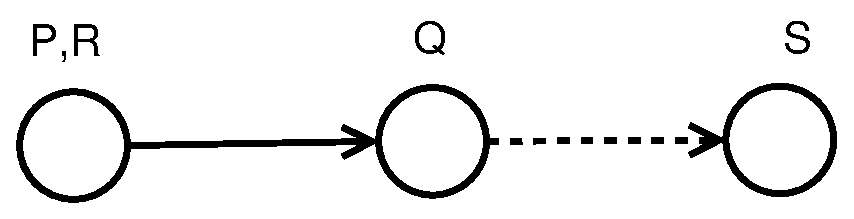
\includegraphics[scale=.4]{diagrams/Impl_1.eps} 
%&
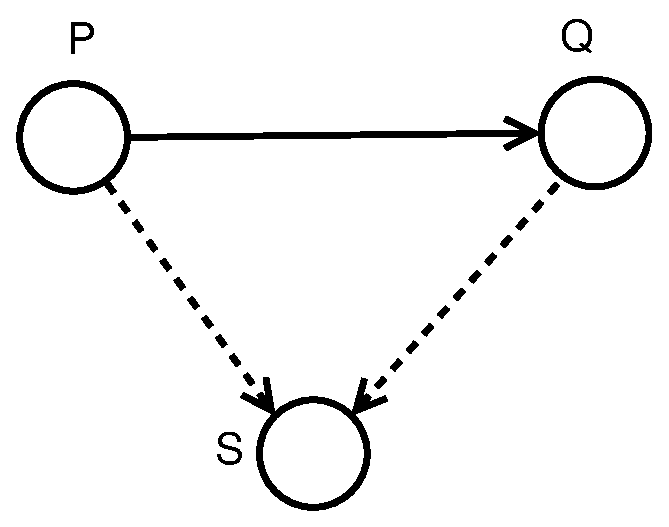
\includegraphics[scale=.4]{diagrams/Impl_2.eps} %& 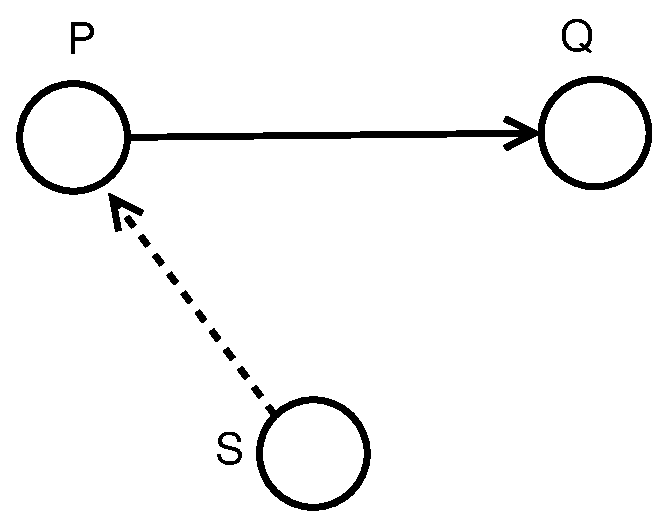
\includegraphics[scale=.4]{diagrams/Impl_3.eps} \\
 %\footnotesize (a) %& \footnotesize (b) 
\end{tabular}
\caption{Heap graphs}  \label{fig:Eq5_example}
\end{center}
\end{figure}

%Consider the assignment of $D_F^{\dgen}[\myr,\s]$ where $\s \not= \p,\ \myr \not\in   \{\p, \q\}$ .What if $\myr$  and $\p$ are aliases then it would 
%be equal to $\num{D_F^{\din}[\q, \s]} \star \epsilonset$ giving incorrect information although there is a path via field $\f$ to $\s$.Fig:~\ref{fig:Eq5_example}(a)
%gives us a picture of how it is.Hence when $\myr$ and $\p$ are aliases  $D_F^{\dgen}[\myr,\s]$ is assigned to $\num{D_F^{\din}[\q, \s]} \star \fieldI{f}{}{1}$.Hence
%its modified as 
%
%
%
%
%
%$D_F^{\dgen}[\myr, \s] = \left\{\begin{array}{@{}ll}
%\num{D_F^{\din}[\q, \s]} \star \fieldI{f}{}{1} & \epsilon \in D_F^{\din}[\myr,\p]  \\
%\num{D_F^{\din}[\q, \s]} \star
%D_F^{\din}[\myr, \p] & \mbox{Otherwise}
%%\end{array}\right.$  $\s \not= \p,\ \myr \not\in \{\p, \q\}$ \\
%
%
%    
%    \quad \quad  For the data flow equation of $I_F^{\dgen}[\p, \q]$ there are two modifications.For the first one assume a self loop is present at $\p$ through field $\f$ .
%And a statement of form $\p \rightarrow \f = \myr$ is encountered.Then according to the previous version of this data flow equation $I_F^{\dgen}[\p, \myr]$ would be
%$\{(\fieldD{f}{}, \epsilon)\} \cup ( \fieldI{f}{}{1} \times \epsilonset)$ ,because of which we wrongly infer that there are two paths through which $\p$ and $\myr$
%intersect.This information at some cases can make our analysis conservative by reporting p as a DAG even though its a TREE.For this reason we modify the equations as
%$\{(\fieldD{f}{}, \epsilon)\}
%  \cup ((1 \star (\remOne{D_F^{\din}[\p,
%      \p]}{ \{\project{D_F^{\din}[\p,\p]}{f} \cup \epsilonset \} })) \times \epsilonset)$ \\



Consider the heap graph in Fig:~\ref{fig:Eq5_example}, you can notice that the heap nodes pointed by $\p$ and $\q$ interfere at $\q$ as well as
at $\s$. The latter part is not captured by  $I_F^{\dgen}[\p, \q]$ i.e 

$I_F^{\dgen}[\p, \q]$ = $\{(\fieldD{f}{}, \epsilon)\}
  \cup ((1 \star (\remOne{D_F^{\din}[\p,
      \p]}{ \{\project{D_F^{\din}[\p,\p]}{f} \cup \epsilonset \} })) \times \epsilonset)$

This equation is not considering the effect when both $\p$ and $\q$ reach some node pointed by $\s$ at which they interfere. 
To handle this case we look at the  set of all heap pointer's $\s$ which is not equal to $\p$ or $\q$ but has paths to it from $\p$ and $\q$.
Going by the definition of Interference matrix we find the fields through which these two pointers interfere, which is nothing but
$D_F^{\din}[\p,\s] \times D_F^{\din}[\q,\s]$. The Union of all such elements for each $\s$ constitute our final information. Thus

  $\{(\fieldD{f}{}, \epsilon)\}
  \cup ((1 \star (\remOne{D_F^{\din}[\p,
      \p]}{ \{\project{D_F^{\din}[\p,\p]}{f} \cup \epsilonset \} })) \times \epsilonset) \cup  \I$ \\
  \quad \quad where \ 
  $\I  =   \bigcup_{s\in\heap,\s \not= \p,\q } \{ {D_F^{\din}[\p,\s] \times D_F^{\din}[\q,\s] \ \vert \  \ \num{D_F^{\din}[\p,\s]} >1 , \num{D_F^{\din}[\q,\s]} >1} \}$  \\

%Let us look at the equation $I_F^{\dgen}[\s, \q]  = (1 \star D_F^{\din}[\s, \p]) \times \epsilonset,\ \s \not\in \{\p, \q\}$.Consider the case where
%$\s$ and $\p$ are aliases,in that case above equation would yield $( (1 \star \epsilonset ) \times \epsilonset)$ ,which is obviously incorrect as can be inferred from  Fig:~\ref{fig:Eq5_example}(c).
%We know that they interfere using the field  $\f$ ,so its assigned to $\fieldI{f}{}{1} \times \epsilonset$ when they are aliases.Finally the equation is 
%
%	  $I_F^{\dgen}[\s, \q] = \left\{\begin{array}{@{}ll}
%	  \fieldI{f}{}{1} \times \epsilonset &  \epsilon \in D_F^{\din}[\s,\p] \\
%	  (1 \star D_F^{\din}[\s, \p]) \times
%	  \epsilonset  & \mbox{Otherwise}
%	  \end{array}\right.$  $\s \not \in \{\p, \q\}$ \\
%     
%    \quad \quad Similar to the above case is the one involving $I_F^{\dgen}[\s, \myr]$ where $\s$ is alias of $\p$ and $\myr$ is alias of $\q$ .So when these sets of pointers are aliases we
%assign $\{ \fieldI{f}{}{1},\epsilon \}$ else the old equation stays. \\
% $\s \not\in \{\p, \q\},\ \myr \not\in \{\p,\q\},\ \s \not= \myr$ \\
%	    $I_F^{\dgen}[\s, \myr] = \left\{\begin{array}{@{}ll}
%	    \{ \fieldI{f}{}{1},\epsilon \} & \{\epsilon \in D_F^{\din}[\s,\p],\epsilon \in D_F^{\din}[\myr,\q] \} \\
%	    (1 \star D_F^{\din}[\s, \p])
%	    \times \{\beta\  \vert\ (\alpha, \beta) \in I_F^{\din}[\q,
%	      \myr]\} & \mbox{Otherwise}  
%	  \end{array}\right.$ \\
%	  
%
%Now let us shift our attention to the Boolean variables and equations.Whatever information that is generated for $\p$ and $\q$ should be reflected on their aliases.
%For the Boolean equations we do the below 
%
%$\begin{array}{l}
%\{x_{cycle}^{gen} = p_{cycle}^{gen}[p/s],x_{cycle}^{gen} = p_{cycle}^{gen}[p/s] \} \ \ 
%if \  \epsilon \in D_F^{\din}[\x,\p] \\
%\{x_{cycle}^{gen} = q_{cycle}^{gen}[q/s],x_{cycle}^{gen} = q_{cycle}^{gen}[q/s] \} \ \ 
%if \ \epsilon \in D_F^{\din}[\x,\q]  
%\end{array}$ \  $\forall \x \in \heap, \x \not= \p,\q$ \ \\  
%
%This is for the Boolean variables
%
%$\begin{array}{l}
%  f_{\x\y} = \true  \ \ if \epsilon \in D_F^{\din}[\x,\p],\epsilon \in D_F^{\din}[\y,\q] \\
%  f_{\p\y} = \true  \ \ if \epsilon \in D_F^{\din}[\y,\q] \\
%  f_{\x\q} = \true  \ \ if \epsilon \in D_F^{\din}[\x,\p]
%\end{array}$ \ $\forall \x , \y  \in \heap, \x \not= \p,\y \not= \q$  \\ 

      
\item{\tt p = q $\rightarrow$ f}:
	
	Let up consider the sample code given below. After statement {\tt S2} both \p\ and \q\ will be pointing to the same heap structure.
{\small \tt
\begin{center}
    \begin{tabular}[b]{l}
      S1. y$\rightarrow$f = x; \\
      S2. y = y$\rightarrow$f; \\
    \end{tabular}
\end{center}
  }
  
	At the end of statement {\tt S1}, $D[y,x]$ would contain the entry $\fieldD{f}{}$. Hence at statement {\tt S2}, $D_1[y,x]$ is assigned
$\upath$, but if we could somehow find that $x$ and $y$ are aliases after this statement we could escape this
approximation and assign $\epsilon$ to  $D_1[y,x]$. After any statement $\p = \q \rightarrow \f$, $\p$ will be pointing to that node which is 
directly reachable from $\q$ through field $\f$. If there is any pointer $\s$ which is reachable from $\q$ directly or indirectly through field $\f$ 
that node would be reachable from $\p$ also. But as 
we don't know through which field $\p$ can reach $\s$, $\upath$ is assigned to $D_1[\p,\s]$.
\[
	D_1[\p, \s] =  \upath \quad  
	\forall \s \in \heap, \s \not=\p \wedge
	\project{D_F^{\din}[\q, \s]}{f} \not= \emptyset
	\]
But if we consider only those $\s$ which can be directly reachable from  $\q$, it would simply be an alias for $\p$ and in that case
we could just assign $\epsilon$ to $D_1[\p,\s]$. For this we need to check whether $\project{D_F^{\din}[\q, \s]}{f} = f^{\drct}$, if true then
$\s$ and $\p$ are aliases after the statement. This change for $D_1[\p, \s]$is reflected below

	$\forall \s \in \heap, \s \not=\p$ \\
	$D_1[\p, \s] =  \left\{\begin{array}{@{}ll}
	                        \upath & \{ \project{D_F^{\din}[\q, \s]}{f} - f^{\drct} \} \not= \emptyset \\
				\{ \epsilon \} & \project{D_F^{\din}[\q, \s]}{f} = f^{\drct}
	                       \end{array}\right.$ 
\\

After {\tt p = q $\rightarrow$ f} there will be a path from $\q$ to $\p$ through field $\f$. This is reflected in the equation
${D_2[\q,\p]} = \{ f^{\drct}\} \cup (\infty \star (\remOne{D_F^{\din}[\q, \q]}{\epsilonset})) \cup \upath$.
We can also see $\upath$ appended at the end, this was added because we were not sure if there was another path by which $\q \rightarrow \f$ can 
be reached from $\q$ .
One observation here is that, if there was a path other than through $\f$ that the heap node pointed by $\q \rightarrow \f$ is reachable from heap node
pointed by $\q$ then shape at $\q$ would have been a DAG or a CYCLE. So when the shape at $\q$ is a TREE initially there would be just
one path from node pointed by $\q$ to node pointed by $\q \rightarrow \f$ and that is through $\f$ only. Writing the same thing according to 
our data flow values

 $if \q \not = \p$  \\
 ${D_2[\q,\p]} = \left\{\begin{array}{@{}ll}
	f^{\drct} & q_{in}^{dag}=\false, q_{in}^{cycle}=\false \\
	\{ f^{\drct}\} \cup (\infty \star (\remOne{D_F^{\din}[\q, \q]}{\epsilonset})) \cup \upath &  \mbox{Otherwise} 
	\end{array}\right.$  \\ \\
	%\quad \quad When we look at  $D_2[\s, \p]$ ,it can be noticed that the case where $\s$ and $\q$ being aliases is not considered.If it is then the equation will have to modified 
%in a similar way as done for ${D_2[\q,\p]}$.What ever happened to $\q$ will now happen to $\s$ .

%  $D_2[\s, \p] = \left\{\begin{array}{@{}ll}
%  \left\{\begin{array}{@{}ll}
%   f^{\drct} & s_{in}^{tree}=\true \\ \\
%   \{ f^{\drct}\} \cup (\infty \star (\remOne{D_F^{\din}[\s, \s]}{\epsilonset})) \\ \cup \upath & \mbox{Otherwise}  \\
%  \end{array}\right. &  \epsilon \in D_F^{\din}[\s,\q] \\
%  \infty \star D_F^{\din}[\s, \q] & \mbox{Otherwise}
%  \end{array}\right.$  \\
%\quad \quad $\forall \s \in \heap, \s \not=\q$ \\
%   The Boolean variables also has to be fixed considering the aliases of $\q$. \\
%	$\forall \x \in \heap, \x \not= \p,\q$  $f_{\x\p} = \true \ \ if \epsilon \in D_F^{\din}[\x,\q]$

\end{itemize}

\begin{figure}[h]
\begin{tabular}{c} 
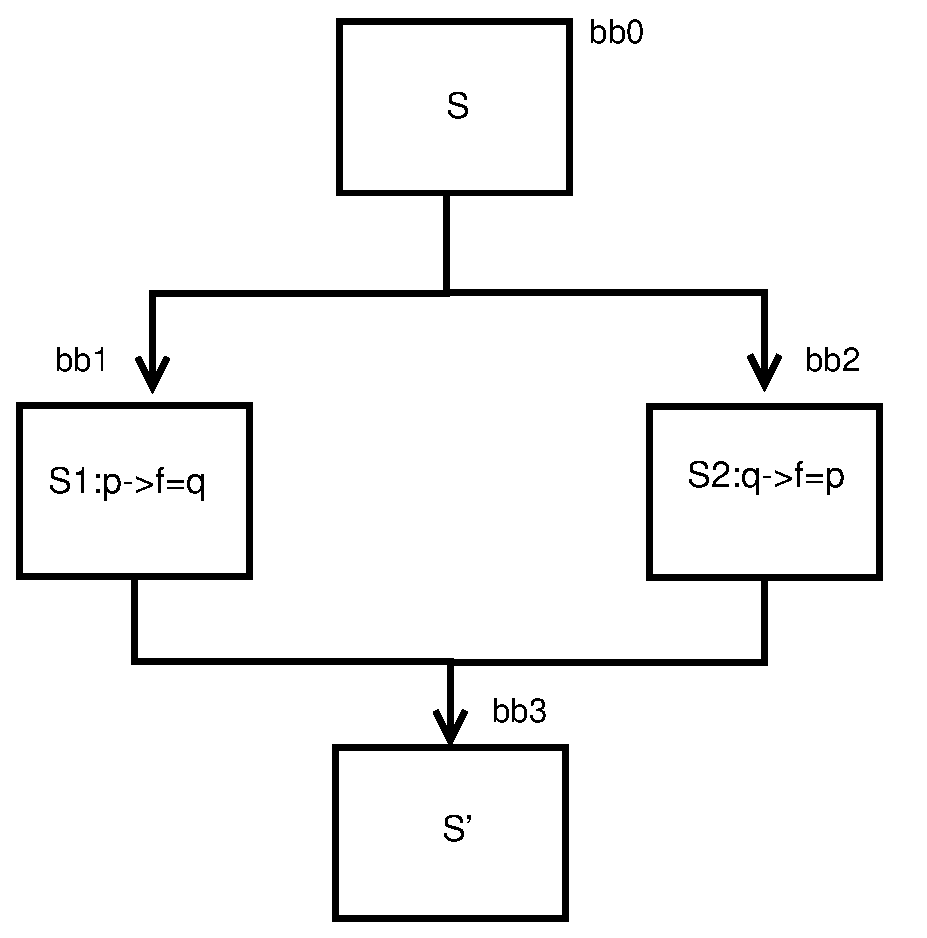
\includegraphics[scale=.35]{diagrams/Enhancements_d1.eps}
\\
\footnotesize (a)Control flow graph  \\ \\

 \scalebox{0.80}{
\begin{tabular}[h]{|l@{}|@{}c@{}|@{}c@{}|} \hline
 {\bf Basic} & $D_F$ & $I_F$ \\ 
 {\bf block} & & \\ \hline

{\tt $OUT(bb1)$} & 
\begin{tabular}{|p{3mm}|p{22mm}p{22mm}|} \hline 
            & $\p$  		& $\q$   \\ \hline
  $\p$ 	& $\epsilon$	& $\{\fieldD{f}{}\}$	 \\ \hline
  $\q$ 	& $\emptyset$	& $\epsilon$	\\ \hline
\end{tabular}
 &
\begin{tabular}{|p{3mm}|p{45mm}p{45mm}|} \hline 
            & $\p$  		& $\q$   \\ \hline
  $\p$ 	& $\{(\epsilon,\epsilon)\}$	& $\{(\fieldD{f}{}, \epsilon)\}$	 \\ \hline
  $\q$ 	& $\{(\epsilon,\fieldD{f}{}) ) \}$	& $\{(\epsilon,\epsilon)\}$	\\ \hline
\end{tabular} \\ \hline

{\tt $OUT(bb2)$} & 
\begin{tabular}{|p{3mm}|p{22mm}p{22mm}|} \hline 
            & $\p$  		& $\q$   \\ \hline
  $\p$ 	& $\epsilon$	& $\emptyset$	 \\ \hline
  $\q$ 	& $\{\fieldD{f}{}\}$ 	& $\epsilon$	\\ \hline
\end{tabular}
 &
\begin{tabular}{|p{3mm}|p{45mm}p{45mm}|} \hline 
            & $\p$  		& $\q$   \\ \hline
  $\p$ 	& $\{(\epsilon,\epsilon)\}$	& $\{ (\epsilon),\fieldD{f}{} )\}$ 	 \\ \hline
  $\q$ 	& $\{(\fieldD{f}{}, \epsilon)\}$ 	& $\{(\epsilon,\epsilon)\}$	\\ \hline
\end{tabular} \\ \hline

{\tt $IN(bb3)$} & 
\begin{tabular}{|p{3mm}|p{22mm}p{22mm}|} \hline 
            & $\p$  		& $\q$   \\ \hline
  $\p$ 	& $\epsilon$	& $\{\fieldD{f}{}\}$	 \\ \hline
  $\q$ 	& $\{\fieldD{f}{}\}$	& $\epsilon$	\\ \hline
\end{tabular}
 &
\begin{tabular}{|p{3mm}|p{45mm}p{45mm}|} \hline 
            & $\p$  		& $\q$   \\ \hline
  $\p$ 	& $\{(\epsilon,\epsilon)\}$	& $\{(\fieldD{f}{}, \epsilon),(\epsilon,\fieldD{f}{} ) \}$	 \\ \hline
  $\q$ 	& $\{(\fieldD{f}{}, \epsilon),(\epsilon,\fieldD{f}{} ) \}$	& $\{(\epsilon,\epsilon)\}$	\\ \hline
\end{tabular} \\ \hline
\end{tabular}
}
\\ \\
\footnotesize (b)Direction and Interference Matrices \\ \\

\scalebox{0.80}{
\begin{tabular}[b]{|c@{}|@{}c|}\hline
  Basic Block \  & Boolean Equations \\ \hline
 OUT(bb1) &
% \begin{tabular}{c}
$(f_{\p\q} \wedge \InC{q}) \vee (f_{\p\q} \wedge (\num{\DFM{\q}{\p}} \geq 1))$ \\ \hline

OUT(bb2) &
$(f_{\q\p} \wedge (\num{\DFM{\q}{\p}} \geq 1))$ \\ \hline

IN(bb3) & 
$((f_{\p\q} \wedge \InC{q}) \vee (f_{\p\q} \wedge (\num{\DFM{\q}{\p}} \geq 1)) \cup (f_{\q\p} \wedge (\num{\DFM{\q}{\p}} \geq 1)))$ \\ \hline
\end{tabular} 
} \\  

\footnotesize (c)Boolean equation of {\tt $p_{cycle}$}  \\
\end{tabular}
\caption{DataFlow values and CFG} \label{if-else-cfg}
\end{figure}

\textbf{Information Passed to successors: }
Here we will discuss about the less precise results that we are obtaining while passing the boolean equations to its successorss according to 
\cite{Sandeep}. Also we will discuss ways to fix this.
Let us look at the Fig:~\ref{if-else-cfg}(a), it contains a single statement in the if and else blocks.
The Direction matrices at the OUT of bb1 and bb2 are shown in Fig:~\ref{if-else-cfg}(b).
 
$f_{\p\q}$ and $f_{\q\p}$  are TRUE from basic blocks bb1 and bb2 respectively. Now if we look at the equation of {\tt $p_{cycle}$} at IN(bb3) 
from Fig:~\ref{if-else-cfg}(c) and substitute the data flow values at IN(bb3) from  Fig:~\ref{if-else-cfg}(b) we can see that it evaluates to TRUE,
inferring that the shape of \p\ as CYCLE even though its a TREE in reality. The problem here is we are not taking into consideration that only one of the 
basic blocks among bb1, bb2 will be executed.
Merging of these boolean equations does not capture that effect.

\textbf{Solution: }For this problem we propose a simple and effective solution which even reduces the memory consumption
by a good amount. What we propose is, at any statement when we evaluate a boolean equation and pass it to its successor only if that equation
evaluates to 1 otherwise we do not pass it to the successor at all. This solution works because at those basic statements which can change the heap shape,
such as $\p \rightarrow \f =\q$, whatever boolean equations are generated they alone are sufficient to determine the shape of each pointer at that program 
point.
  \begin{eqnarray*}
  S1: \q \rightarrow \g &=& \p \\
  S2: \p \rightarrow \f &=& \q   
  \end{eqnarray*}
Lets take a simple example of just two statements. 
As equations at {\tt S1} evaluates to false and hence no boolean equation is passed to {\tt S2}. It means the value of  $\InC{\p}$ for {\tt S2} 
is FALSE and $\OutC{\p}$ of {\tt S2} is same as $\GenC{\p}$ of {\tt S2}. The equation for $\GenC{\p}$, which is the same given in Fig:~\ref{if-else-cfg}(c) first row 
evaluates to TRUE hence detecting the shape correctly as a CYCLE. 

There is one case where boolean equation is to be changed to get correct results 
which is for $\GenD{p}$ of statement $\p \rightarrow \f =\q$.
\begin{eqnarray*}
	  \GenD{p}   &=&  ( f_{\p\q} \wedge (\num{\IFM{\p}{\q}} > 1) )
\end{eqnarray*}
Consider the set of statements  
\begin{eqnarray*}
  S1: \x \rightarrow \f &=& \y \\
  S2: \x \rightarrow \g &=& \y  \\
  S3: w \rightarrow \f &=& \x 
\end{eqnarray*}
After the first two statements a DAG is formed at $\x$. After the third statement a link is created from  $w$ to $\x$ via field $\f$, that means $w$ also points to a DAG. 
As the shape of $w$ before this statement was a TREE, $\InD{w}$ is empty according to the above mentioned change. We know that $\KillD{w}$ is also $\false$ for this statement, 
hence $\OutD{w}$ is nothing but $\GenD{w}$. Now consider the equation of $\GenD{w}$, it is equal to $( f_{w\x} \wedge (\num{\IFM{w}{\x}} > 1) )$. The value of 
boolean variable $f_{w\x}$ is $\true$ but value of $(\num{\IFM{w}{\x}} > 1) )$ is $\false $ as the entry $\IFM{w}{\x}$ would just contain 
$\{ \fieldD{f}{} , \epsilon \}$ . Finally evaluating the value of $\OutD{w}$ to $\false$, which is incorrect.
  
If at all we have used the old approach of passing information to successors then $\InD{w}$ would not have been empty, and would have successfully identified
the shape at $w$ as a DAG. Now to overcome this problem we have to change to the equation of $\GenD{p}$. Whenever a statement $\p \rightarrow \f = \q$ is
encountered and shape of $\q$ before this statement is a DAG, then we can simply say that $\p$ also points to a DAG. This is formalized as
\begin{eqnarray*}
	  \GenD{p}   &=&  (f_{\p\q} \wedge \InD{q}) \vee ( f_{\p\q} \wedge (\num{\IFM{\p}{\q}} > 1) )
\end{eqnarray*}

\textbf{Limitation: }This change in $\GenD{p}$ will cause loss of accuracy in one scenario (also exhibited by Ghiya et al.~\cite{Ghiya96}), but 
as a whole it has a lot of advantages in accuracy and memory consumption, so we have adopted this change. Lets look at that particular scenario.

\begin{figure}
\centering
\begin{tabular}{cc}
\begin{tabular}{c}
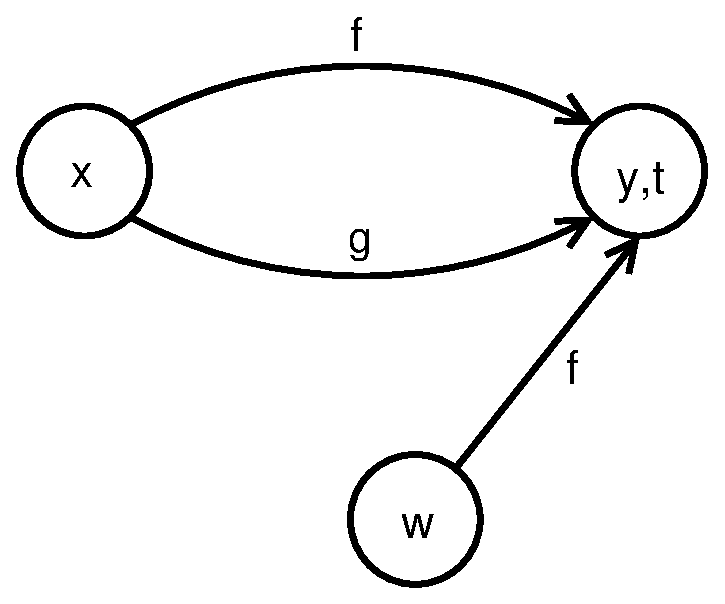
\includegraphics[scale=.4]{diagrams/Enhancements_d3.eps}
\end{tabular} & 
\begin{tabular}{c}
S1: $\x \rightarrow \f = \y$ \\
S2: $\x \rightarrow \g = \y$  \\
S3: $t = \x \rightarrow \g$ \\
S4: $w \rightarrow \f = t$
\end{tabular} \\
\footnotesize (a)Heap Graph & \footnotesize (b)Set of statements
\end{tabular}
\caption{ Example with Heap graph and Set of statements} \label{fig:enhancements_example}
\end{figure}

 
Refer to Fig:~\ref{fig:enhancements_example}, the effect of the set of statements are shown in the heap graph.
After the second statement a DAG is formed at $\x$ and when the third statement is encountered the equation of $\x$ is copied to the equation of $t$.
And at statement S4 the shape at $w$ is reported as a DAG. When this change in $\GenD{p}$ was not incorporated, the shape was reported as a TREE.
The details about how this change is making the shape vary is shown below.


(According to the original equation of $\GenD{\p}$ )

After S1: \\
$\OutD{x} = False$

After S2: \\
$\OutD{x} =  ( f_{\x\y} \wedge (\num{\IFM{\x}{\y}} > 1) )$
(which evaluates to TRUE)

After S3: \\
$\OutD{t} = ( f_{\x\y} \wedge (\num{\IFM{\x}{\y}} > 1) )$
(which evaluates to TRUE)

After S4:\\
$\OutD{w} = ( f_{wt} \wedge (\num{\IFM{w}{t}} > 1) )$ 
(which evaluates to FALSE) \\ \\
(According to the new equation of $\GenD{\p}$ )

After S4: \\
$\OutD{w} =   (f_{wt} \wedge \InD{t}) \vee ( f_{wt} \wedge (\num{\IFM{w}{t}} > 1) )$
(which evaluates to TRUE) \\

The new version of equation of $\OutD{w}$ evaluates to TRUE because of the term $\InD{t}$ which is also TRUE. As this part
was not present in the previous version of $\GenD{p}$ it correctly infers the shape of $w$ as Tree.

\section{Final Data Flow Equations}
All the modifications that were proposed are shown in  Fig:~\ref{fig:Modified Data Flow Equations}. It contains the 
final set of data flow values for each of the statements.

Let us first introduce some notations which will be used frequently in the following analysis.

$\forall \p \in \heap, \mbox{we introduce two notations } \alias{P} \mbox{ and }  \alias{p} as$ 
\begin{eqnarray*}
	\alias{P} &=& \aliasinfo{\p} \mbox{ and } \\
	\alias{p} &\in& \alias{P}
\end{eqnarray*}


\begin{figure} 
\begin{spacing}{2.0}
\begin{tabular}{|p{2.6cm}|p{12cm}|}
\hline
 {\tt p = malloc()} & 

\scalebox{0.70}{
  \begin{tabular}{lll}
	  \KillC{p}  = \InC{p} & \KillD{p} = \InD{p} &\\
	  \GenC{p} = \false  & \GenD{p} = \false &\\

	  $\forall \s \in \heap,\ \s \not= \p,$ && \\
	  $D_F^{\dkill}[\p,\s]$  =  $D_F^{\din}[\p,\s]$ & $D_F^{\dkill}[\s,\p]$  =  $D_F^{\din}[\s,\p]$ & $D_F^{\dkill}[\p,\p]$  =  $D_F^{\din}[\p,\p]$ \\
	  $D_F^{\dgen}[\p,\s]$   =  $\emptyset$         & $D_F^{\dgen}[\s,\p]$   =  $\emptyset$          &$D_F^{\dgen}[\p,\p]$   =  $\epsilonset$ \\
	  $I_F^{\dkill}[\p,\s]$  =  $I_F^{\din}[\p,\s]$ & $I_F^{\dkill}[\p,\p]$  =  $I_F^{\din}[\p,\p]$   &\\
	  $I_F^{\dgen}[\p,\s]$   =  $\emptyset$         & $I_F^{\dgen}[\p,\p]$   =  $\epsilonpairset$     &
\end{tabular}
} \\
\hline
 {\tt p = NULL} & 
\scalebox{0.70}{
  \begin{tabular}{ll}
	  \KillC{p}  = \InC{p} & \KillD{p} = \InD{p} \\
	  \GenC{p} = \false    & \GenD{p} = \false \\

	   $\forall \s \in \heap,$ & \\
	  $D_F^{\dkill}[\p,\s]$  =  $D_F^{\din}[\p,\s]$ & $D_F^{\dkill}[\s,\p]$  =  $D_F^{\din}[\s,\p]$ \\
	  $D_F^{\dgen}[\p,\s]$    =  $\emptyset$  & $D_F^{\dgen}[\s,\p]$    =  $\emptyset$ \\
	  $I_F^{\dkill}[\p,\s]$  =  $I_F^{\din}[\p,\s]$ & $I_F^{\dgen}[\p,\s]$    =  $\emptyset$ 
  \end{tabular}
} \\
\hline
\begin{tabular}{l}
{\tt p = q} \\
{\tt p =\&(q$\rightarrow$f)} \\
{\tt p = q op n}
\end{tabular}
 &
\scalebox{0.70}{
\begin{tabular}{l}

	\KillC{p} = \InC{p} \quad\qquad \KillD{p} = \InD{p} \\ 
	\GenC{p}   = \InC{q}[q/p] \quad \GenD{p} = \InD{q}[q/p] \\ 
	where $X[\q / \p]$ creates a copy of $X$ with all occurrences
	of $\q$ replaced by $\p$.\\

      $\forall \s \in \heap,  \s \not= \p,  \forall f \in \fields,$ \\

	$f_{\p\s} = f_{\q\s}$  \quad  $f_{\s\p} = f_{\s\q}$ \\
	$D_F^{\dkill}[\p, \s]$  =  $D_F^{\din}[\p, \s]$ \quad $D_F^{\dkill}[\s, \p]$  =  $D_F^{\din}[\s, \p]$ \quad $D_F^{\dkill}[\p, \p]$  =  $D_F^{\din}[\p, \p]$ \\
	$D_F^{\dgen}[\p, \s]$    =  $D_F^{\din}[\q, \s]$ \quad $D_F^{\dgen}[\s, \p]$    =  $D_F^{\din}[\s, \q]$ \quad $D_F^{\dgen}[\p, \p]$    =  $D_F^{\din}[\q, \q]$  \\
	$I_F^{\dkill}[\p, \s]$  =  $I_F^{\din}[\p, \s]$ \qquad $I_F^{\dgen}[\p, \s]$    =   $I_F^{\din}[\q, \s]$ \\
	$I_F^{\dkill}[\p, \p]$  =  $I_F^{\din}[\p, \p]$ \qquad $I_F^{\dgen}[\p, \p]$    = $I_F^{\din}[\q, \q]$ 
  \end{tabular}
} \\
\hline
\tt{ $\delta$ = p }
&
\scalebox{0.70}{
    \begin{tabular}{l}
	$\GenC{\delta}   = \InC{\p}[\p/\delta] \qquad\qquad \GenD{\delta} = \InD{\p}[\p/\delta]$ \\
	$\forall \s \in \heap, \s \not= \p, \forall f \in \fields$ \\
	$\KillC{\s} = \InC{\s}  \qquad\qquad\qquad  \KillC{\s} = \InD{\s}$  \\
	$\GenC{\s}  = \InC{\s}[\p/\delta] \qquad\qquad   \GenD{\s} = \InD{\s}[\p/\delta]$ \\ 	 
	where $X[\q / \p]$ creates a copy of $X$ with all occurrences
	of $\q$ replaced by $\p$. \\
	$\forall \s \in \heap, \s \not= \p, \forall f \in \fields$ \\
	$f_{\delta\s} = f_{\p\s}$  \quad  $f_{\s\delta} = f_{\s\p}$ \\
	$D_F^{\dgen}[\delta,\s]$    =  $D_F^{\din}[\p,\s]$ \quad  $D_F^{\dgen}[\s,\delta]$    =  $D_F^{\din}[\s,\p]$ \quad  
		 $D_F^{\dgen}[\delta,\delta]$    =  $D_F^{\din}[\p,\p]$  \\
	 $I_F^{\dgen}[\delta,\s]$    =   $I_F^{\din}[\p,\s]$ \quad \; $I_F^{\dgen}[\delta,\delta]$    = $I_F^{\din}[\p,\p]$  \\  
    \end{tabular}
} \\
\hline
\end{tabular}
\end{spacing}
\end{figure}

\begin{figure}[p]
\begin{spacing}{2.0}
\begin{tabular}{|p{2.6cm}|p{12cm}|}
\hline
{\tt p$\rightarrow$f=null}
&
	\scalebox{0.70}{
	  \begin{tabular}{l}
	  \KillC{p}  = \false, \quad \KillD{p} = \false \\
	  \GenC{p} = \false, \quad \GenD{p} = \false  \\
		$\forall \q,\s \in \heap, \s \notin \alias{P}$ \\
	  $f_{\alias{p}\q}$ = \false \\
	  $D_F^{\dkill}[\alias{p}, \q]$  = $\project{D_F^{\din}[\p, \q]}{f}$ \qquad  \;  ${D_{F}^{{\dkill}}[\s, \q]}  = \emptyset  $  \\
 	  $I_F^{\dkill}[\alias{p}, \s] = \{(\alpha,  \beta) \ \vert\ (\alpha, \beta) \in I_F^{\din}[\p,  \q] \mbox, \ \alpha \equiv f^\anysup \}$ \\ 
 	  ${I_F^{\dkill}[\q, \s]} = \emptyset \mbox{ if } \q \notin \alias{P}$ \qquad\qquad   
 	  ${I_F^{\dkill}[\alias{p}, \alias{p}]} = \{(\alpha,  \beta) \ \vert\ (\alpha, \beta) \in I_F^{\din}[\p,  \p] \mbox, \ \alpha \equiv f^\anysup \}$
  \end{tabular}
} \\
\hline
{\tt p$\rightarrow$f = q}
&
    \scalebox{0.70}{
    \begin{tabular}{l}
	  \mbox{The KILL relations are same as that of {\tt p$\rightarrow$f = null}} \\
	  $\GenC{\p}   =  (f_{\p\q} \wedge \InC{q}) \vee (f_{\p\q} \wedge (\num{\DFM{\q}{\p}} \geq 1))$  \quad 
	  $\GenD{p}   =  (f_{\p\q} \wedge \InD{q}) \vee ( f_{\p\q} \wedge (\num{\IFM{\p}{\q}} > 1) )$ \\
 	  $\GenC{q}   = f_{\p\q} \wedge (\num{\DFM{\q}{\p}} \geq 1)$ \quad\qquad\qquad\qquad\quad $\GenD{q} = \false$\\ 
	  $f_{\alias{p}\alias{q}} = \true$ \\
%-------------------------------------------------------Newly Added-----------------------------------------------------------------------------

%	 $\GenC{\x}   =  \GenC{\p}[\p/\x] \qquad\qquad \GenD{\x} = \GenD{\p}[\p/\x]\ \forall \x \in \alias{P}$\\
%	 $\GenC{\x}   =  \GenC{\q}[\q/\x] \qquad\qquad \GenD{\x} = \GenD{\q}[\q/\x]\ \forall \x \in \alias{Q}$\\

% DO NOT DELETE
%The above rule said that if x alias to p then create a similar eqn for x. But there might be cases like x alias to p and also to q but p and q are not
%aliases. Like
% if{x = p} else {x=q}  p->f = q; Here the corresponding eqn will be x(c) = f(xq) and D[qx]>=1 whih will be true but inreality x is not cycle.
% this is mitigates by the below eqns.

	  $\GenC{\s} =  ((\num{\DFM{\s}{\p}} \geq 1) \wedge f_{\p\q} \wedge \InC{q})$ $\vee\ ((\num{\DFM{\s}{\p}} \geq 1) \wedge f_{\p\q} \wedge
 	  (\num{\DFM{\q}{\p}} \geq 1))$ \\ 
	  \quad  $\vee\ ((\num{\DFM{\s}{\q}} \geq 1) \wedge f_{\p\q}
	  \wedge (\num{\DFM{\q}{\p}} \geq 1))$, \ \   $\forall \s \in \heap, \s \not= p,q $\\
	  $\GenD{\s}   = (\num{\DFM{\s}{\p}} \geq 1) \wedge
	  f_{\p\q} \wedge (\num{\IFM{\s}{\q}} > 1)$, \ $\forall \s \in \heap, \s \not= p,q $\\


%-----------------------------------------------------------------------------------------------------------------------------------------
% 	 $ D_F^{\dgen}[\myr, \s] = \num{D_F^{\din}[\q, \s]} \star              %modified as
% 	  D_F^{\din}[\myr, \p],\ \s \not= \p,\ \myr \not\in
% 	  \{\p, \q\} $\\ 	

 $ D_F^{\dgen}[\myr, \s] = \num{D_F^{\din}[\q, \s]} \star  D_F^{\din}[\myr, \p],\ \s \notin \alias{P},\ \myr \notin \alias{P},\ \myr \notin \alias{Q}$ \\
%-----------------------------------------------------------------------------------------------------------------------------------------
	  $D_F^{\dgen}[\myr, \alias{p}] = \num{D_F^{\din}[\q,\p]} \star D_F^{\din}[\myr, \p], \ \myr \notin \alias{P}$\\
	  $D_F^{\dgen}[\alias{p}, \myr] = \num{D_F^{\din}[\q, \myr]} \star (\remOne{D_F^{\din}[\p, \p]}{\epsilonset} \cup \{f^{\indrct 1}\})$, \ \  $\myr \notin \alias{Q}$ \\ 
	  $D_F^{\dgen}[\alias{p}, \alias{q}] = \{\fieldD{f}{}\}\ \cup\ (\num{D_F^{\din}[\q, \q] - \epsilonset} \star \{\fieldI{f}{}{1}\})\ \cup\ (\num{D_F^{\din}[\q, \q]} \star ( \remOne{D_F^{\din}[\p, \p]}{\{\project{D_F^{\din}[\p,\p]}{f} \cup \epsilonset \}}))$ \\ 
	  $D_F^{\dgen}[\alias{q}, \alias{q}] = 1 \star D_F^{\din}[\q, \p]$ \\
	  $D_F^{\dgen}[\alias{q}, \myr] = \num{D_F^{\din}[\q, \myr]} \star D_F^{\din}[\q, \p],\ \myr \notin \alias{P},\ \myr \notin \alias{Q}$ \\ 
%-----------------------------------------------------------------------------------------------------------------------------------------
% 	  $I_F^{\dgen}[\p, \q] = \{(\fieldD{f}{}, \epsilon)\}                   %modified as
% 	  \cup ((1 \star (\remOne{D_F^{\din}[\p,
% 	      \p]}{\epsilonset})) \times \epsilonset)$ \\
	  
	  $I_F^{\dgen}[\alias{p}, \alias{q}] = \{(\fieldD{f}{}, \epsilon)\}
	  \cup ((1 \star (\remOne{D_F^{\din}[\p,
      \p]}{ \{\project{D_F^{\din}[\p,\p]}{f} \cup \epsilonset \} })) \times \epsilonset) \cup  \I$ \\
 	  \quad \quad where \ 
 	  $\I  =   \bigcup_{\x\in\heap,\x \notin \alias{P},\alias{Q} } \{ {D_F^{\din}[\p,\x] \times D_F^{\din}[\q,\x] \ \vert \  \ \num{D_F^{\din}[\p,\x]} >1 , \num{D_F^{\din}[\q,\x]} >1} \}$ \\
%-----------------------------------------------------------------------------------------------------------------------------------------
	  
	  $I_F^{\dgen}[\alias{p}, \myr]$ = 
 	  $(1 \star (\remOne{D_F^{\din}[\p, \p]}{\epsilonset})) \times 
	  \{\beta\ \vert\ (\alpha, \beta) \in I_F^{\din}[\q, \myr] \}$  
	  $\cup\ \{f^\drct\} \times 
	  \{\beta\ \vert\ (\epsilon, \beta) \in I_F^{\din}[\q, \myr] \}$ \\
	  \quad \quad  $\cup\ \{f^{\indrct 1}\} \times 
	   \{\beta\ \vert\ (\alpha, \beta) \in I_F^{\din}[\q, \myr],
	  \alpha \not= \epsilon \}$, 
	  $\qquad \qquad \myr \notin \alias{P}, \alias{Q}$ \\


%-----------------------------------------------------------------------------------------------------------------------------------------
% 	  $I_F^{\dgen}[\s, \q] = (1 \star D_F^{\din}[\s, \p]) \times   %modified as
% 	  \epsilonset,\ \s \not\in \{\p, \q\}$ \\
	  
 	  $I_F^{\dgen}[\s, \alias{q}] = (1 \star D_F^{\din}[\s, \p]) \times 
 	  \epsilonset,\ \s \notin \alias{P},\ \alias{Q}$ \\

%-----------------------------------------------------------------------------------------------------------------------------------------

 %-----------------------------------------------------------------------------------------------------------------------------------------
% 	  $I_F^{\dgen}[\s, \myr] = (1 \star D_F^{\din}[\s, \p])           % modified as
% 	  \times \{\beta\ \vert\ (\alpha, \beta) \in I_F^{\din}[\q,
%  	    \myr]\}$,
% 	    $ \qquad \s \not\in \{\p, \q\},\ \myr \not\in \{\p,
% 	  \q\},\ \s \not= \myr$

 	  $I_F^{\dgen}[\s, \myr] = (1 \star D_F^{\din}[\s, \p])           % modified as
 	  \times \{\beta\ \vert\ (\alpha, \beta) \in I_F^{\din}[\q,
  	    \myr]\}$,
 	    $ \qquad \s \not\in \alias{P},\alias{Q},\ \myr \not\in \alias{P},\alias{Q},\ \s \not= \myr$ \\
  \end{tabular}
 }  \\
\hline
\end{tabular}
\end{spacing}
\end{figure} 



\begin{figure}[p]
\begin{spacing}{2.0}
\begin{tabular}{|p{2.6cm}|p{12cm}|}
\hline
{\tt p = q$\rightarrow$f} &
    \scalebox{0.70}{
    \begin{tabular}{l}
	The KILL relations are same as that of {\tt p = NULL} \\
	$\GenC{p} = \InC{q} \qquad \GenD{p} = \InD{q}$ \\

	$f_{\alias{q}\p} = \true$ \quad
	${h_{\p\myr}} =
	\num{\project{D_F^{\din}[\q,\myr]}{f}} \geq 1\quad
	\forall h \in \fields, \forall \myr \in \heap$  \\

	$ \upath \quad=\quad \epsilonset \cup \ \bigcup_{f\in\fields} \{f^{\drct},
	f^{\indrct\infty}\}$  \\ \\

	$\forall \s \in \heap, \s \not=\p$ \\
	$D_1[\p, \s] =  \left\{\begin{array}{@{}ll}
	                        \upath & \{ \project{D_F^{\din}[\q, \s]}{f} - f^{\drct} \} \not= \emptyset \\
				\{ \epsilon \} & \project{D_F^{\din}[\q, \s]}{f} = f^{\drct}
	                       \end{array}\right.$
	\quad
	$D_1[\p, \p] = \left \{ \begin{array}{@{}ll}
	  \upath& \q.\shape \mbox{ evaluates to } \Cycle \\
	  \epsilonset & \mbox{Otherwise}
	\end{array}. \right. $  \\
	$I_1[\p, \p] = \upath \times \upath $ \\ \\

%-----------------------------------------------------------------------------------------------------------------------------------------
% 	${D_2[\q,\p]} = \{ f^{\drct}\} \cup (\infty \star (\remOne{D_F^{\din}[\q, \q]}{\epsilonset})) \cup \upath$  \\   modified as
	${D_2[\alias{q},\p]} = \left\{\begin{array}{@{}ll}
	f^{\drct} & q_{in}^{tree}=\true \\
	\{ f^{\drct}\} \cup (\infty \star (\remOne{D_F^{\din}[\q, \q]}{\epsilonset})) \cup \upath &  \mbox{Otherwise} 
	\end{array}\right.$  \ \  $if \q \not = \p$ \\ 

  $D_2[\s, \p] = \infty \star D_F^{\din}[\s, \q]$ \quad $\forall \s \in \heap, \s \notin \alias{Q},\ \s \not=\p$ \\

	$I_2[\s, \p] = D_2[\s, \p] \times \epsilonset \quad \forall \s \in \heap $	\\ \\


	$D_3[\s, \p] = \{ \alpha \ \vert \ (f^{\drct}, \alpha) \in I_F^{\din}[\q, \s] \}$  \\
	$I_3[\s, \p] = \{\alpha \ \vert\ (f^\anysup, \alpha) \in I_F^{\din}[\q, \s]\} \times \upath$ \\ \\

	Final $I_F$ and $D_F$ relations are: \\

	$D_F^{\dgen}[\myr, \s] =  D_1[\myr, \s] \cup D_2[\myr, \s] \cup D_3[\myr, \s] \quad \forall\myr,\s \in \heap$  \\
	$I_F^{\dgen}[\myr, \s] =  I_1[\myr, \s] \cup I_2[\myr, \s] \cup I_3[\myr, \s] \quad \forall\myr,\s \in \heap$   \\
    \end{tabular}
  } \\
\hline

\end{tabular}
\end{spacing}
\caption{Modified Data Flow Equations}  \label{fig:Modified Data Flow Equations}
\end{figure} 



\chapter{Subset Based Analysis \label{Subsetbased}}
Sometimes data structures include auxiliary fields that are useful for traversing the data structure
for debugging or diagnostic purposes. The presence of such fields, however can result in the more conservative shape.
To illustrate this we present the following example .

\section{Motivating Example}

\begin{example}
Consider the code segment in Program.~\ref{MotivatingExample} which has functions for searching data in a binary tree and 
inserting node into the same. The fields of structure {\tt Node}, which is used to realize the functions, are also shown. The 
structure {\tt Node} has three field pointers {\tt Left}, {\tt Right} and {\tt Parent}.
In the {\tt insert} function we can see a cycle getting created due to the lines {\tt S5} and {\tt S6}.
Take a look at Fig:~\ref{fig:Code} to see how the field sensitive analysis also
gets the shape of  \p  \ and  \s \ as a cycle at that point.

Now in the {\tt search} function, the {\tt Parent} pointer is
not at all used, so ideally the shape that is actually traversed inside the {\tt search} function is a Tree. But as the function is called
with the root of the tree, whose shape gets evaluated to Cycle in the {\tt insert} function,
we infer that the shape of the root as Cycle in the {\tt search} function as well even though the parent link is never been traversed. 
\end{example}
        
%  \begin{center}
% 
\begin{figure}
\begin{lstlisting}[caption={Motivating Example} ,label=MotivatingExample]
Struct Node {
  Struct Node *Left,*Right,*Parent;
  int key;
};
typedef Struct Node Node;

bool search(Node *root,int key){
if(root)
  return (key==root->key)||search(root->Left,key)||search(root->Right,key);
return 0;
}


void insert(Node *root,int key){
    Node *s=root;   //This pointer is used for traversing the Tree 
    ..
    //New node is inserted as a child of s(s can be any node of the tree)
    Node *p;
    S1. p=(Node *)malloc(sizeof(Node));    	
    S2. p->Left=NULL;			
    S3. p->Right=NULL;			
    S4. p->key=key;				
    S5. s->Left=p;				
    S6. p->Parent = s;			
    ..
}

\end{lstlisting}
\end{figure}

% \end{center}

\begin{figure}[h]
\centering
\begin{tabular}{@{}c@{}}

  \scalebox{0.80}{
    \begin{tabular}[b]{|c||c|c|}
          \hline 
          {\bf After} & $\Left_{p,t}$ & $\Parent_{t,p}$ \\ 
           \hline \hline
	  {\tt S1}       & false	  & false     \\ \hline
	  {\tt S2}       & false          & false     \\ \hline
	  {\tt S3}       & false 	  & false     \\ \hline
	  {\tt S5}       & true	          & false     \\ \hline
          {\tt S6}       & true	          & true     \\ \hline
    \end{tabular} 
      
  } \\
  \footnotesize (a) Boolean Variables  \\ \\
  

  \scalebox{0.80}{
\begin{tabular}[b]{|l@{}|@{}c@{}|@{}c@{}|} \hline
 {\bf After} & $D_F$ & $I_F$ \\ 
 {\bf Stmt} & & \\ \hline

{\tt S1} & 
\begin{tabular}{|p{3mm}|p{22mm}p{22mm}|} \hline 
            & $\p$  		& $\s$   \\ \hline
  $\p$ 	& $\epsilon$	& $\emptyset$	 \\ \hline
  $\s$ 	& $\emptyset$	& $\emptyset$	\\ \hline
\end{tabular}
 &
\begin{tabular}{|p{3mm}|p{45mm}p{45mm}|} \hline 
            & $\p$  		& $\s$   \\ \hline
  $\p$ 	& $\{(\epsilon,\epsilon)\}$	& $\emptyset$	 \\ \hline
  $\s$ 	& $\emptyset$	& $\emptyset$	\\ \hline
\end{tabular} \\ \hline

{\tt S2} & 
\begin{tabular}{|p{3mm}|p{22mm}p{22mm}|} \hline 
            & $\p$  		& $\s$   \\ \hline
  $\p$ 	& $\epsilon$	& $\emptyset$	 \\ \hline
  $\s$ 	& $\emptyset$	& $\emptyset$	\\ \hline
\end{tabular}
 &
\begin{tabular}{|p{3mm}|p{45mm}p{45mm}|} \hline 
            & $\p$  		& $\s$   \\ \hline
  $\p$ 	& $\{(\epsilon,\epsilon)\}$	& $\emptyset$	 \\ \hline
  $\s$ 	& $\emptyset$	& $\emptyset$	\\ \hline
\end{tabular} \\ \hline

{\tt S3} & 
\begin{tabular}{|p{3mm}|p{22mm}p{22mm}|} \hline 
            & $\p$  		& $\s$   \\ \hline
  $\p$ 	& $\epsilon$	& $\emptyset$	 \\ \hline
  $\s$ 	& $\emptyset$	& $\emptyset$	\\ \hline
\end{tabular}
 &
\begin{tabular}{|p{3mm}|p{45mm}p{45mm}|} \hline 
            & $\p$  		& $\s$   \\ \hline
  $\p$ 	& $\{(\epsilon,\epsilon)\}$	& $\emptyset$	 \\ \hline
  $\s$ 	& $\emptyset$	& $\emptyset$	\\ \hline
\end{tabular} \\ \hline

{\tt S5} & 
\begin{tabular}{|p{3mm}|p{22mm}p{22mm}|} \hline 
            & $\p$  		& $\s$   \\ \hline
  $\p$ 	& $\epsilon$	& $\emptyset$	 \\ \hline
  $\s$ 	& $\{\fieldD{Left}{}\}$	& $\emptyset$	\\ \hline
\end{tabular}
 &
\begin{tabular}{|p{3mm}|p{45mm}p{45mm}|} \hline 
            & $\p$  		& $\s$   \\ \hline
  $\p$ 	& $\{(\epsilon,\epsilon)\}$	& $\{( \epsilon,\fieldD{Left}{})\}$ 	 \\ \hline
  $\s$ 	& $\{(\fieldD{Left}{}, \epsilon)\}$	& $\emptyset$	\\ \hline
\end{tabular} \\ \hline

{\tt S6} & 
\begin{tabular}{|p{3mm}|p{22mm}p{22mm}|} \hline 
            & $\p$  		& $\s$   \\ \hline
  $\p$ 	& $\epsilon$	& $\{\fieldD{Parent}{}\}$	 \\ \hline
  $\s$ 	& $\{\fieldD{Left}{}\}$	& $\emptyset$	\\ \hline
\end{tabular}
 &
\begin{tabular}{|p{3mm}|p{45mm}p{45mm}|} \hline 
            & $\p$  		& $\s$   \\ \hline
  $\p$ 	& $\{(\epsilon,\epsilon)\}$	&  $\{( \epsilon,\fieldD{Left}{}),(\fieldD{Parent}{},\epsilon)\}$	 \\ \hline
  $\s$ 	& $\{(\fieldD{Left}{}, \epsilon),(\epsilon,\fieldD{Parent}{})\}$		& $\emptyset$	\\ \hline
\end{tabular} \\ \hline

\end{tabular} 

}  \\
 \footnotesize (b) Direction ($D_F$) and Interference ($I_F$) matrices  \\ \\
  


\scalebox{0.80}{
\begin{tabular}[b]{|c@{}|@{}c|}\hline
  Heap Pointer & Boolean Equations \\ \hline
{\tt $p_{cycle}$} & \{  ($\Parent_{p,s}  \wedge  False $) $\vee$ ($\Parent_{p,s} \wedge ( \num{D[s,p]} >= 1)$) \} $\vee$    \{ $\Left_{s,p}  \vee ( \num{D[p,s]} >= 1)$ \}  \\  \hline
{\tt $p_{dag}$} & \{ ($\Parent_{p,s} \wedge   ( \num{I[p,s]} > 1)$) \} \\ \hline 
{\tt $s_{cycle}$} & \{ $\Parent_{p,s} \wedge ( \num{D[s,p]} >= 1)$ \} $\vee$ \{  ($\Left_{s,p}  \wedge  False $) $\vee$ ($\Left_{s,p} \wedge   ( \num{D[p,s]} >= 1)$) \} \\ \hline
{\tt $s_{dag}$} & \{ ($\Left_{s,p} \wedge   ( \num{I[s,p]} > 1)$) \} \\ \hline
\end{tabular} 
} \\
\footnotesize (c) Boolean Equations after S6  \\    

\end{tabular}

\caption{Data Flow Values at each statement for Program.~\ref{MotivatingExample} }\label{fig:Code}
\end{figure}

For the above case, unlike the Field Sensitive Analysis, Subset Based Analysis can  identify the shape as Tree by considering the fields used by a 
function and using only those fields to infer the shape. Subset based analysis is a way in which only a subset of field pointers accessed in a 
function are used to get more precise shape information. We now present the details of the analysis.

\section{Analysis}    
The Field Sensitive Analysis needs to be modified slightly for the subset based analysis to occur.
During pre-processing of code, we parse each function separately and create a set of fields associated with each of them. This set will contain
all the field pointers that are used at least once in the function. We use $S_F$ to denote the subset of fields used by function \F.
For the functions present in  Program.~\ref{MotivatingExample}

\begin{center}
$S_{insert}$ = \{ Left , Right , Parent \} \\
$S_{search}$ = \{ Left , Right \} \\ 
\end{center}

During the evaluation of the boolean equations for function \F, we restrict our analysis to the fields that are present in $S_F$.
In this modified analysis when we reach a statement in \F\ we have to modify the evaluation of equations according to the following rules.

Any boolean equation would generally contain the  terms like $f_{\p\q}$,\ \DFM{\p}{\q},\ \IFM{\p}{\q}.
We replace each of the these terms by $f_{\p\q}^{\#} , {D^{\#}[p,q]} ,{I^{\#}[p,q]}$ respectively. Now lets 
understand what each of these terms mean.

\begin{itemize}

 \item $f_{\p,\q}^{\#}$ :
	  This term will have a value as False if  $\f$ is not accessed at any point in function \F, i.e $\f \not \in S_F$ 
If its present then the value is same as that of $f_{\p,\q}$
\begin{eqnarray*}
f_{\p,\q}^{\#} &=&  \left \{ \begin{array}{@{}ll}
                       f_{\p,\q}  & \f \in S_F  \\
			 \false & \mbox{Otherwise}
                       \end{array} \right.
\end{eqnarray*}

  \item ${D^{\#}[p,q]}$ :
      It contains the first field of all the paths that start from $\p$ and end at $\q$ except those whose first fields are not present in $S_F$.
In other way this is nothing but the difference of the contents of $D[p,q]$ and the set of all first fields for the paths from $\p$ to $\q$ whose
first fields are not present in $S_F$.

\begin{eqnarray*}
D^{\#}[\p, \q] &=& D[\p, \q] -\bigcup_{ \f \in \fields,\f \not \in S_F } \{  \project{D[\p,\q]}{f}         \}
\end{eqnarray*}

\item ${I^{\#}[p,q]}$ :
      Very similar to the way how $D^{\#}[\p, \q]$ was defined this term is also defined.      
\begin{eqnarray*}
I^{\#}[\p, \q] &=& I[\p, \q] - \bigcup_{ \f \in \fields,\f \not \in S_F } \{  \project{I[\p,\q]}{f}         \}
\end{eqnarray*}
\end{itemize}

After making all these replacements we evaluate the equation to get the shape.
Now that we have all the details about the analysis, lets look at how it works for the above mentioned motivating example.

% small code snippet present in Fig.~\ref{fig:SampleCode_Info}(a).

\begin{example}
 The function {\tt search} would be called with the root of the Tree as the parameter.
In Program.~\ref{MotivatingExample} that the variable {\tt root} is assigned to {\tt s} in the insert function. So at the end of the
insert function whatever boolean equation {\tt s} would have, {\tt root} also would have the same except replacing every {\tt s} by {\tt root} in the equation.
Actually the insert function may be recursive or iterative, if we consider the equation of {\tt s} at the end of complete insert function
it would be very large and explaining would be a lot difficult. So we have considered the equation only at the end of statement {\tt S6}. 
From Fig:~\ref{fig:Code}(c). the the boolean equation of {\tt root} is derived as 
\begin{eqnarray*}
{\tt root_{cycle}} &=& \{ \Parent_{p,root} \wedge ( \num{D[root,p]} >= 1) \} \vee \{  (\Left_{root,p}  \wedge False) \vee \\
 && (\Left_{root,p} \wedge   ( \num{D[p,root]} >= 1)) \} \\
{\tt root_{dag}} &=&  \{ (\Left_{root,p} \wedge   ( \num{I[root,p]} > 1)) \} 
\end{eqnarray*}

Even with the dataflow values concerning the Boolean variables, Direction and Interference matrices, {\tt root} would have the same values corresponding to that
of {\tt s} at the end of statement {\tt S6}. Hence at the start of  {\tt search} function $\Left_{root,p} = \true , \Parent_{p,root} = \true$  while the matrices are as given below.  \\

\scalebox{0.80}{
\begin{tabular}[b]{|@{}c@{}|@{}c@{}|} \hline
\begin{tabular}{|p{6mm}|p{22mm}p{22mm}|} \hline 
   D         & $\p$  		& $root$   \\ \hline
  $\p$ 	& $\epsilon$	& $\{\fieldD{Parent}{}\}$	 \\ \hline
  $root$ 	& $\{\fieldD{Left}{}\}$	& $\emptyset$	\\ \hline
\end{tabular}
 &
\begin{tabular}{|p{6mm}|p{45mm}p{45mm}|} \hline 
   I         & $\p$  		& $root$   \\ \hline
  $\p$ 	& $\{(\epsilon,\epsilon)\}$	&  $\{( \epsilon,\fieldD{Left}{}),(\fieldD{Parent}{},\epsilon)\}$	 \\ \hline
  $root$ 	& $\{(\fieldD{Left}{}, \epsilon),(\epsilon,\fieldD{Parent}{})\}$		& $\emptyset$	\\ \hline
\end{tabular} \\ \hline
\end{tabular} 
}

\par
Before going into the search function we need to know the small change this function undergoes when represented in intermediate form(GIMPLE) on which the
analysis takes place. The function would transform to

\begin{figure}[h]
\begin{lstlisting}
bool search(Node *root,int key){
       Node *temp1,*temp2;
       int tempInt;
St1:   temp1=root->left;
St2:   temp2=root->right;
       tempInt=root->key
       if(root)
         return (key==tempInt)||search(tmep1,key)||search(temp2,key);
       return 0;
}
\end{lstlisting}
\end{figure}

At the statement {\tt St1} first time the boolean equation will be evaluated for this function. We are not considering the evaluation after {\tt St2} because it would be done in the same way as that of {\tt St1}. 
As $\GenC{temp1} = \InC{root}$ and $\KillC{temp1} = \InC{temp1}$,  
$\OutC{temp1}$ is same as $\InC{root}$. Now lets look at each term in $\InC{root}$ and find what it evaluates to in the subset based analysis. 
\begin{eqnarray*}
 Parent_{p,root}^{\#} &=& \false  \ \ \ (Parent \not \in S_{Search} ) \\
 Left_{root,p}^{\#} &=& Left_{root,p} \  (Left \in S_{Search} ) \\
 D^{\#}[root,p] &=& D[root,p] - \project{D[root,p]}{Parent} \\
		&=& D[root,p] - \phi \\
		&=& \{\fieldD{Left}{}\} \\
 D^{\#}[p,root] &=& D[p,root] - \project{D[p,root]}{Parent} \\
		&=& D[p,root] - \{\fieldD{Parent}{}\} \\
		&=& \phi
\end{eqnarray*}

Substituting these above values in the equation of $\InC{root}$ would result in $\false$. In the similar way when we try to evaluate $\InD{root}$ it would give us $\false$, thus rightly detecting the shape of data structure traversed
as Tree.
\end{example}

\par
Note that the subset based analysis increases the precision at the cost of extra computation required to compute $D^{\#} ,I^{\#}$ and $f^{\#}$.
Due to the lack of sufficient benchmarks its not very clear to us if and when this overhead can be threat by the gain in precision. More work is required to evaluate this trade off.


% {\red
% \section{Limitations}
% In the Field sensitive analysis only the first field information in a path between two labelled nodes are present in the matrices, and 
% we are using that information in our subset based analysis. But this information is not always sufficient to get the exact shape 
% (considering the fields accessed in a function).To get the accurate results the information about the set of all fields that are being used in a path 
% is required or in other way we need the complete information about the heap graph. As this is very difficult to gather
% so we will end up with less precise (but conservative) results. We present one such example of safe result.
% \begin{example}
% Consider the heap graph in Fig.~\ref{Subset_fig}. This heap graph contains 3 unlabeled nodes and 2 labeled nodes. Assume that the solid edges are 
% constructed in {\tt main} function and the dotted edge is the last one to be constructed in some function {\tt foo} called from {\tt main}. Also assume 
% that in the {\tt foo} function, field $\f$ is the only one that is accessed.
% When the statement $Q \rightarrow \f = P$ is encountered in {\tt foo} the following data flow boolean equation is generated.
% \begin{eqnarray*}
% \GenC{Q}   &=&  (f_{QP} \wedge \InC{P}) \vee (f_{QP} \wedge (\num{\DFM{P}{Q}} \geq 1)) 
% \end{eqnarray*}
% In the second term of the above disjunction, the value of the cell  $\DFM{P}{Q}$ would be  $\{ \fieldI{f}{}{1} \}$ as there is only one path from $P$ 
% to $Q$ and it starts by field $\f$. No information is available about the presence of $\g$ field in that path, and $D^{\#}[P,Q]$ evaluates 
% to $\{ \fieldI{f}{}{1} \}$ making the value of $\GenC{Q}$ as TRUE. So even though in the function the field $\g$ is not accessed, but
% a cycle is formed using that field we are reporting it as a cycle.
% \end{example}
% 
% \begin{figure}[h]
% \centering
% \begin{tabular}{c}
%  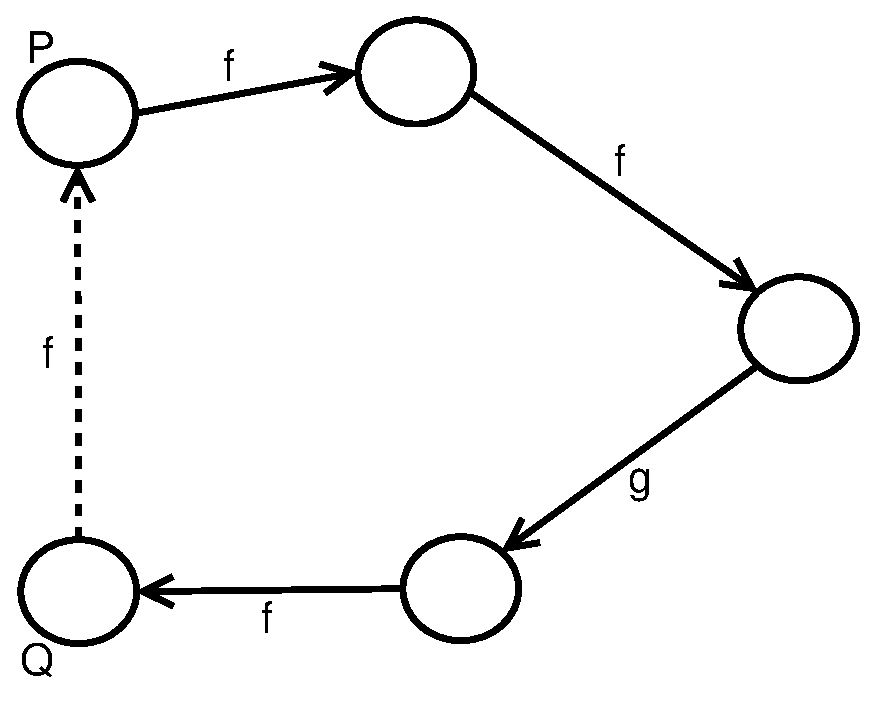
\includegraphics[scale=.3]{diagrams/Subset_11.eps} 
% \end{tabular}
% \caption{heap graph} \label{Subset_fig} 
% \end{figure}
% 
% }
% 



\chapter{Inter Procedural Analysis\label{Interprocedural}}
Every programmer knows the importance of procedures and how vastly they are used in programs, so for any analysis 
to be effective handling procedures is very important. Just going by intra procedural analysis causes lot of information loss because we have to make
worst case assumptions at the time of function calls. In Inter procedural analysis we have to take care of call-return, parameter passing
local variables, recursion etc. apart from the work done in intra procedural analysis.

There are two variants of Interprocedural analysis, Context Sensitive 
and Context Insensitive. In Context Sensitive only interprocedural valid paths are considered during the data flow
unlike Context insensitive in which some invalid paths also may be considered. Lets look at a small example.

\begin{example}
Consider a program in which {\tt main} function has 2 call statements for the function {\tt p1}.
Fig:~\ref{fig:Some}(a) is a global control flow graph containing control flow graph of both procedures
and considering each call statement as a goto from that statement to the start of the called procedure,
similarly treating each return statement as goto from that statement to the instruction following
the call statement by which this function was called. Just for the sake of clarity
we have introduced return blocks after each call statement.

Let the data flow values available just before the call statement {\tt c1} is {\tt df1} and that before {\tt c2}
be {\tt df2}. So {\tt df1} and {\tt df2} would be entering the function {\tt p1} when called at {\tt c1}, {\tt c2} respectively. Similarly
let the corresponding data flow values released out of function be {\tt df1'} and {\tt df2'} respectively.
If we notice the edges between the functions {\tt main} and {\tt p1}, there is a path {\tt c1}, {\tt Enter p1}, {\tt Exit p1}, 
{\tt return p1} (i.e.\ the block below callblock c2); which is not followed in any execution sequence and hence it is not an inter procedurally
valid path. When such paths are considered during data flow imprecise data is obtained leading to
imprecise results. Such an analysis called Context Insensitive,  and  the analysis becomes Context Sensitive when we don't consider such invalid paths.
\end{example}

Fig:~\ref{fig:Some} is a global control graph of small program, but in real life applications the size of this graph
may become very large, so scalability and efficiency get more importance in Inter Procedural Analysis. Hence for some problems 
a compromise may be required between precision and efficiency. We also discuss how our analysis goes about these compromises.
In the next few sections we discuss in detail about one of the context sensitive approach, \textit{Callstring method} and a 
newly proposed method called \textit{shape sensitive approach}.
  
\begin{figure}[h]
 
\begin{tabular}{c  c}
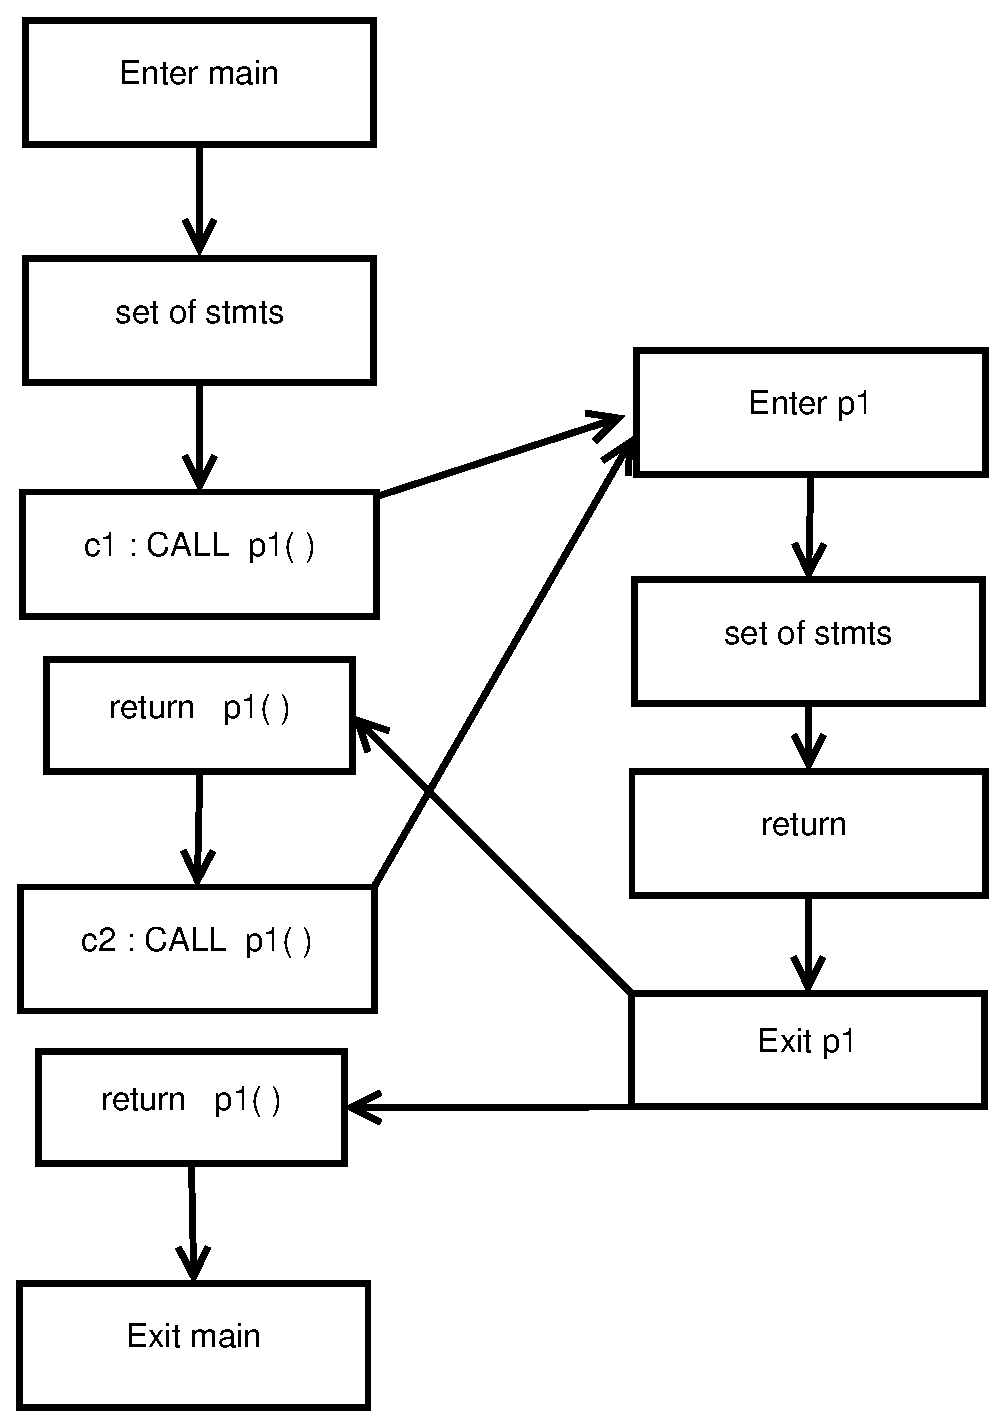
\includegraphics[scale=.4]{diagrams/Diagram1.eps} 
& \   \   \
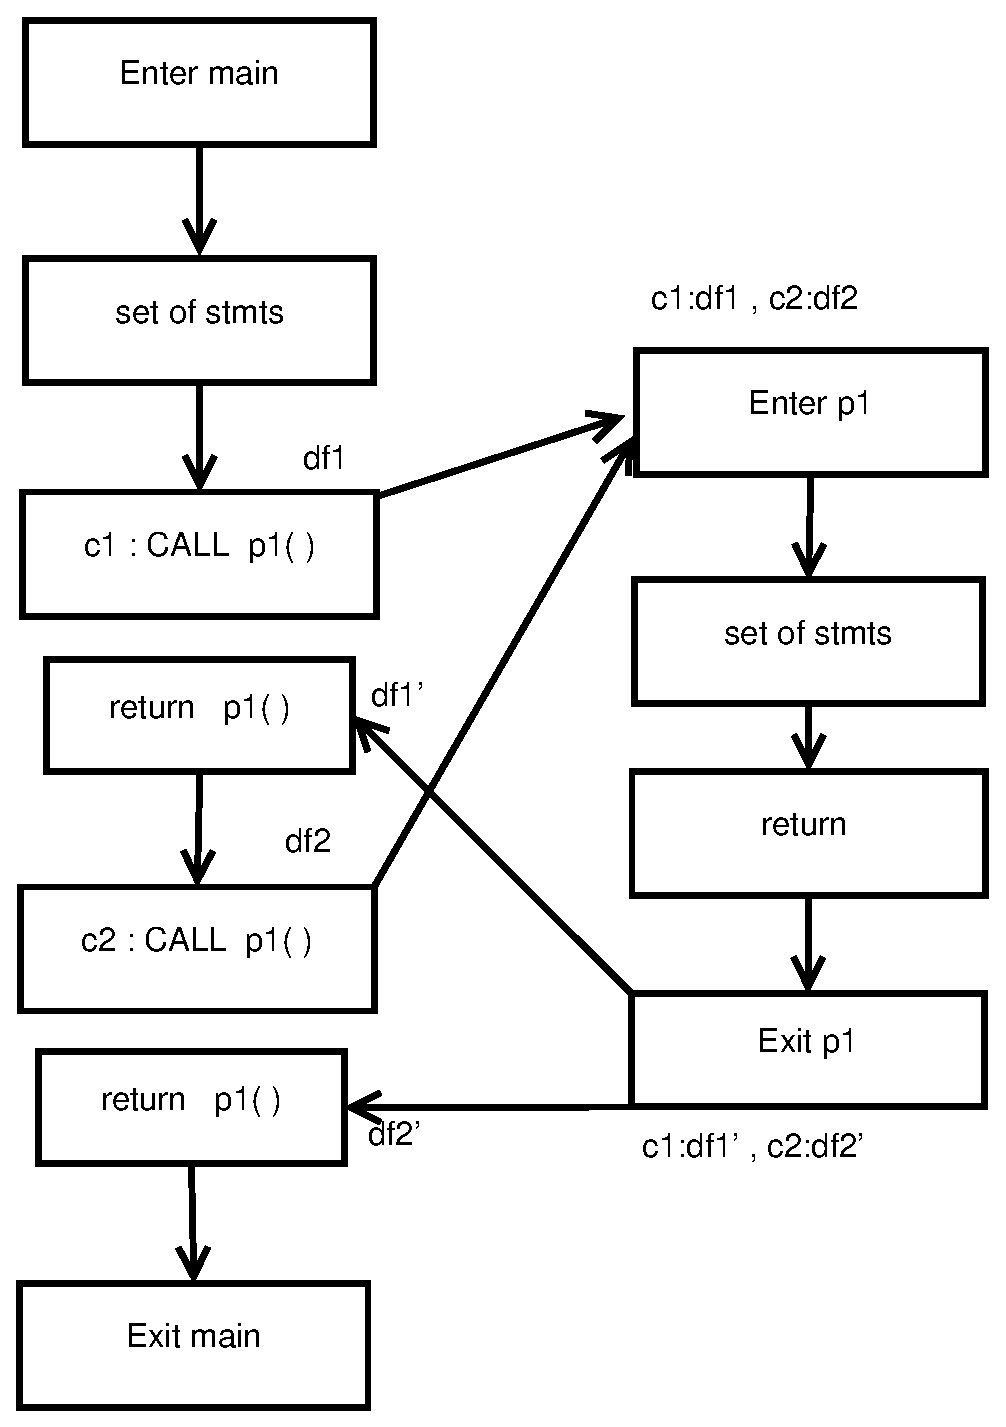
\includegraphics[scale=.4]{diagrams/Diagram12.eps} \\

\footnotesize (a)    & \   \   \  \footnotesize (b)

\end{tabular}

\caption{Global control flow graph}
\label{fig:Some}
\end{figure}
% 
% In this Chapter we discuss what interprocedural analysis method should be considered for implementing the field sensitive analysis of \cite{Sandeep}.
% We have implemented this analysis in two methods, one is Callstring based and other a context insensitive analysis which intelligently
% merges the contexts at function calls.

\section{Callstrings Based Approach}
Callstring Method is one of variants of Context Sensitive Interprocedural Analysis in which along with the data flow values a 
callstring is also propagated. This method of analysis was proposed by Sharir et .al \cite{TwoApproach}. Callstring at 
any program point means the sequence of unfinished procedure calls reaching that point starting form the main functions entry. This 
new tagged information will make the inter procedural analysis explicit, so at return statements information can be validly propagated.
The data flow information at any program point looks like 
  \begin{center}
$<$ Call String cs: Data Flow value d $>$ \\   
  \end{center}
We can notice this representation in Fig.~\ref{fig:Some}(b). Since we know to which call site {\tt df1} and {\tt df2} belongs to, during the 
exit from function {\tt p1}, we can be sure of sending a data flow value to its correct call site. As seen in the figure, {\tt df1'}, {\tt df2'} are 
sent to {\tt c1},{\tt c2} respectively. In this approach only inter procedurally valid paths are used for data flow transfer hence giving more 
precise results. But the problem with this approach is that we have to keep the dataflow values for each callstring
in the memory, leading to increased memory consumption.

Lets discuss an overview of the implementation of call string based interprocedural Field Sensitive analysis. First we process the Control flow
graph. We create separate basic blocks for call statements and also add a new basic block just below call block, i.e.\ the return block.
Then we initialize the global and local worklist's; global worklist contains functions and separate local worklist's are present for each function
which holds basic blocks. For handling termination of call string construction we use the method proposed in \cite{LazyPointer}.

\cite{LazyPointer} use value based termination of call strings. In order to adopt that approach we used a call string map, that 
is present at the start block of each function and maps those data flow tuples whose call string's are different but data flow values are same .
In a way what we are doing is discarding redundant call strings at start of a function.
Consider two call strings ${\sigma}_1$ and ${\sigma}_2$ with same data flow values at the start of some function, both of them need not be 
propagated inside because both of them will anyway undergo the same transitions and generate the same output data flow values at the end of 
function. So we pass only, say the data flow value associated with ${\sigma}_1$, it undergoes some transitions inside the function and some 
dataflow is output at the 
end of the function. This dataflow value is directly copied into the dataflow value associated with ${\sigma}_2$ at the end of function and this 
saves us from processing the same dataflow value associated with ${\sigma}_2$ again.


As mentioned above the memory consumption is more  because we have to maintain separate set of data flow values for each callstring.
This problem with memory is quite an issue in the field sensitive analysis because when we ran the analysis even on a program like merging of linked list 
recursively \cite{linkedlist} the analysis couldn't complete because of large memory consumption. Hence we have moved from Context sensitive to 
Context insensitive.
Though Context insensitive approach takes less memory the accuracy will decrease which is a trade off we have to make.
Further study has to be made about how to design a memory efficient context sensitive analysis for this shape analysis technique.

\section{Shape Sensitive Approach}
In Context Insensitive  analysis we have to compromise on accuracy and in Context Sensitive analysis we have to compromise on memory consumption, so 
if we could find some sort of a middle way approach of both of these, that would be a good gain where both accuracy and memory are optimized. Keeping that in mind we proposed the Shape Sensitive approach.

Lets consider the following scenario in Context Insensitive Analysis. Let we have a function with parameter as a heap pointer. The 
data flow values present at the start of the function when it was called the first time be DF1. At that point shape of that heap 
pointer is a cycle. After a few statements again this function is called and the incoming dataflow values is DF2, let the shape of the same heap pointer now be a tree. Since its a context insensitive 
approach the data entering the function would be DF1 $\cup$ DF2. This also contains DF1 which was responsible for cycle being detected at the first 
time the function was called. So there is a good probability that now also the shape may be inferred as a cycle even though it's not.

So one natural thought that emerges is keep a separate set of data flow values for each shape at the start of functions. This is what we call 
shape sensitive method of context merging. Here what we do is, based on the shape of those heap pointer arguments at that point of function 
call, merging of call contexts happen.
Lets look at this concept by using a small piece of code and later we will show the comparison of this approach with context insensitive approach.

\begin{example}
Consider a function with one parameter which is a heap pointer, the shape of the node pointed to by this can be a TREE, DAG or a CYCLE. For 
such a function we associate an array of data flow values of size three. Let that array be denoted by IN[3]. IN[0] denotes that data flow values 
incoming when the shape at that heap pointer is  a TREE, IN[1] when shape is a DAG and IN[2] when shape is CYCLE. So in the similar way if the 
number of heap pointer parameters are {\tt n} then size of its corresponding IN would be $3^n$ . This size can be adjusted accordingly 
depending on compromise between precision and memory.\\

We also maintain an OUT of the same size as IN which has the data flow values at the end of that function for its corresponding IN.
Now if we look at the sample code given below, the number of parameters is one so size of IN is three. At {\tt c1} the shape of the parameter \p\ 
is a cycle so the incoming values into that function are fed to IN[2] and when the function is returned OUT[2] is updated. Now at {\tt c2} the shape of 
\p\ is a TREE so this time IN[0] and OUT[0] are updated.
\end{example}

\begin{tabular}[t]{cl}
\begin{lstlisting}
struct Node
{
  struct Node *f,*g;
};

void foo(struct Node *s)
{
  struct Node *t;
  S: t=s;
  ....
}
\end{lstlisting}
&
\begin{lstlisting}
int main()
{
  struct Node *p,*q;
  p=(struct Node *)malloc(sizeof(struct Node));
  q=(struct Node *)malloc(sizeof(struct Node));

  S1: p->f=q;
  S2: q->f=p;
  c1: foo(p);
  S3: q->f=NULL;
  c2: foo(p);
}
\end{lstlisting}
\end{tabular}
\\ 
\begin{figure}[h]
\begin{tabular}{c}
 \scalebox{0.7}{
\begin{tabular}{cc}
\renewcommand{\arraystretch}{1.2}
\begin{tabular}[b]{|c|c|c|c|}
\hline
$D_F$     & \p & \q &  \s  \\ \hline \hline 
\p 	& $\{\epsilon\}$ & $\{\fieldD{f}{} \}$ & $\{\epsilon\}$  \\ \hline 
\q             & $\{\fieldD{f}{}\}$      & $\{\epsilon\}$          & $\{\fieldD{f}{}\}$  \\ \hline
\s             & $\{\epsilon\}$           &$\{\fieldD{f}{}\}$      & $\{\epsilon\}$      \\ \hline
\end{tabular} 
&

\renewcommand{\arraystretch}{1.2}
% % \newcommand{\iwd}{0.23\columnwidth}
\begin{tabular}[b]{|c|c|c|c|}
\hline 
$\ I_F$     & $\p$	               & $\q$
&  $\s$              \\ \hline \hline 
%%
$\p$ & $\{ (\epsilon, \epsilon)\}$    & $\{(\fieldD{f}{},\epsilon),(\epsilon,\fieldD{f}{}) \} $   & $\{ (\epsilon, \epsilon)\}$ \\ \hline
$\q$ & $\{(\fieldD{f}{},\epsilon),(\epsilon,\fieldD{f}{}) \} $   & $\{ (\epsilon, \epsilon)\}$ & $\{(\fieldD{f}{},\epsilon),(\epsilon,\fieldD{f}{}) \} $ \\ \hline
$\s$ & $\{ (\epsilon, \epsilon)\}$    & $\{(\fieldD{f}{},\epsilon),(\epsilon,\fieldD{f}{}) \} $   & $\{ (\epsilon, \epsilon)\}$ \\ \hline
\end{tabular} \\
% \caption{C1:Context Insensitive}
\end{tabular}
} \\

\scriptsize (a) C1:IN[2] \\ \\

\scalebox{0.7}{
\begin{tabular}{cc}
\renewcommand{\arraystretch}{1.2}
\begin{tabular}[b]{|c|c|c|c|}
\hline
$D_F$     & \p & \q &  \s  \\ \hline \hline 
\p 	& $\{\epsilon\}$ & $\{\fieldD{f}{} \}$ & $\{\epsilon\}$  \\ \hline 
\q             & $\{\fieldD{f}{}\}$      & $\{\epsilon\}$          & $\{\fieldD{f}{}\}$  \\ \hline
\s             & $\{\epsilon\}$           &$\{\fieldD{f}{}\}$      & $\{\epsilon\}$      \\ \hline
\end{tabular} 
&

\renewcommand{\arraystretch}{1.2}
% % \newcommand{\iwd}{0.23\columnwidth}
\begin{tabular}[b]{|c|c|c|c|}
\hline 
$\ I_F$     & $\p$	               & $\q$
&  $\s$              \\ \hline \hline 
%%
$\p$ & $\{ (\epsilon, \epsilon)\}$    & $\{(\fieldD{f}{},\epsilon),(\epsilon,\fieldD{f}{}) \} $   & $\{ (\epsilon, \epsilon)\}$ \\ \hline
$\q$ & $\{(\fieldD{f}{},\epsilon),(\epsilon,\fieldD{f}{}) \} $   & $\{ (\epsilon, \epsilon)\}$ & $\{(\fieldD{f}{},\epsilon),(\epsilon,\fieldD{f}{}) \} $ \\ \hline
$\s$ & $\{ (\epsilon, \epsilon)\}$    & $\{(\fieldD{f}{},\epsilon),(\epsilon,\fieldD{f}{}) \} $   & $\{ (\epsilon, \epsilon)\}$ \\ \hline
\end{tabular} \\
% \caption{C1:Context Insensitive}
\end{tabular}
} \\
%  
\scriptsize (b) C1:INmap \\ \\

\scalebox{0.7}{
\begin{tabular}{cc}
\renewcommand{\arraystretch}{1.2}
\begin{tabular}[b]{|c|c|c|c|}
\hline
$D_F$     & \p & \q &  \s  \\ \hline \hline 
\p 	& $\{\epsilon\}$ &  & $\{\epsilon\}$  \\ \hline 
\q 	&  & $\{\epsilon\}$ &   \\ \hline 
\s 	& $\{\epsilon\}$ &  & $\{\epsilon\}$  \\ \hline 
\end{tabular} 
&

\renewcommand{\arraystretch}{1.2}
% % \newcommand{\iwd}{0.23\columnwidth}
\begin{tabular}[b]{|c|c|c|c|}
\hline 
$\ I_F$     & $\p$	               & $\q$
&  $\s$              \\ \hline \hline 
%%
$\p$ & $\{ (\epsilon, \epsilon)\}$    &   & $\{ (\epsilon, \epsilon)\}$ \\ \hline
$\q$ &     & $\{ (\epsilon, \epsilon)\}$   &  \\ \hline
$\s$ & $\{ (\epsilon, \epsilon)\}$    &    & $\{ (\epsilon, \epsilon)\}$ \\ \hline
\end{tabular} \\
% \caption{C1:Context Insensitive}
\end{tabular}
} \\

\scriptsize (c) C2:IN[0] \\ \\

\end{tabular}

\caption{Data Flow Values at Function Calls} \label{fig:Inmap}
\end{figure}

\par 
\textbf{Comparison with Context Insensitive}: In Context Insensitive analysis,  we maintain an INmap and OUTmap foreach function, and 
if the incoming data flow values to the function is a subset of present INmap we just pass the OUTmap without processing the function. Otherwise 
we update the INmap by merging incoming dataflow values with  previous INmap and process the function. We will now compare the INmap and IN array  
of both context insensitive and context sensitive approaches and see how the shape is effected at statement {\tt S}.

At {\tt c1} the data flow values at the start of function foo are those in Fig.~\ref{fig:Inmap}(a), since shape of \p\ at that call statement 
is a cycle, so it is assigned to IN[2]. Even if we go by context insensitive it would be the same as shape sensitive given 
in Fig:~\ref{fig:Inmap}(b) denoted by INmap. At statement {\tt S3} cycle gets killed, hence at {\tt c2}, during shape sensitive 
analysis, IN[2] will remain the same as that for {\tt c1}, but now IN[0] is newly created. Just by seeing Fig.~\ref{fig:Inmap}(c) we can see that 
it correctly shows the shape at statement {\tt S} as a TREE. Now if we come to context insensitive, the new INmap during processing of {\tt c2} 
is the union of previous INmap i.e what's present in Fig.~\ref{fig:Inmap}(b) and current incoming data flow values, which same as that present 
in Fig.~\ref{fig:Inmap}(c). So even after merging the INmap would same as earlier. Now just compare Fig.~\ref{fig:Inmap}(b)
and Fig.~\ref{fig:Inmap}(c). According to Fig.~\ref{fig:Inmap}(b) there is a path from $\p$ to $\q$ via field $\f$ and also from $\q$ to$ \p$ via $\f$ but not according to Fig.~\ref{fig:Inmap}(c)
This clearly shows that inside the function foo after {\tt c2} shape of $\p$,$\q$ and $\s$ are identified as cycle for context insensitive 
approach, but shape sensitive conveys the correct shape i.e TREE.

It was told earlier that size of the IN array for each function should be $3^n$ when the number of heap parameters are n for a function, but 
that is not a compulsion.
We can vary the size depending on the preciseness and memory handoff. For example even for a function with 3 parameters (all of them are heap pointers) we 
can keep the size of the array as 3, where IN[0] is used 
when any of the parameter is cycle, IN[1] when none of the parameter is a cycle and at least one is a dag and IN[2] when all of them points to a tree. If 
we go by $3^n$ then the size of the array
would be 9, but now its 3. Though the memory required now is less, information would be accurate in the former case than latter. So the way we choose 
this depends on the constraints we have in terms of memory and preciseness.



\chapter{Implementation And Results \label{Implementation}}
The Interprocedural Field Sensitive Shape Analysis is implemented as a plugin which adds this analysis as one of the passes in GCC.
In the first section a few details about GCC internals are given. Then in the last three sections testing strategy, optimizations and results 
are discussed.

\section{GCC Internals}

\textbf{PLUGINS:}\ Plugin's make the developer add new features to the compiler without modifying the compiler itself.
It is a way of adding, removing and maintaining modules independently. This feature is available from gcc 4.5 and later versions only.
Before we discuss plugins, we present some basic information about GCC architecture. 

The GCC architecture has many passes in it each being either
a GIMPLE, IPA (Interprocedural Analysis) or RTL(Register Transfer Language) pass. So whenever we want to add a pass in GCC we need to talk to the 
pass manager which is located in three files 'passes.c', 'tree-optimize.c' and 'tree-pass.h' and in some way these files need to be modified. And once 
modified we need to build the entire GCC so as to get the pass included in GCC.

But as GCC code base is a very large so it would take lot of time to build each time we change our pass source code. At this 
point plugins make our life easy.
Using plugins we will be able to write a shared object (.so) file that can be loaded into GCC and attached to various stages of
compilation without touching the GCC source code, hence no need of compiling gcc source every time. \\ \\
\textbf{TREE:}\ Tree is the central data structure used by GCC in its internal representation. It can point to a lot of types and to know the particular
type we need to refer TREE\_CODE macro. Each Tree usually have two fields named TREE\_CHAIN and TREE\_TYPE.
While TREE\_CHAIN contains the pointer to next tree (where all the Tree's are arranged in a singly linked list fashion), TREE\_TYPE has information 
about Type or declaration.

\textbf{GIMPLE:} \ Our analysis is performed on the GIMPLE statements which are generated by gcc in its compilation process.
Whenever GCC receives a source file say C source code, the GCC frontend invokes the gimplifier for each function which converts the source code to 
GIMPLE, which is understood by language independent parts of the compiler.
Its actually a 3-address representation with at max one load/store per statement, with memory loads only in RHS and store in LHS of assignment statements.

All the GIMPLE statements that are present in a basic block are in the form of a doubly linked list. Any manipulation to be done on them
require iterators provided by GCC. Our analysis is written as an Inter procedural gcc plugin which operates on the callgraph. In our analysis we 
need to identify whether a particular statement is one among the basic pointer statements.
The example code in Program ~\ref{gimpleAssignment} gives us the details about identifying heap manipulation statement {\tt p = NULL;}. Similarly the other
types of pointer statements are also identified.

\begin{figure}
\begin{lstlisting}[caption={Code to identify pointer statement p = NULL} ,label=gimpleAssignment]
 
if(is_gimple_assign(stmt))
{
    tree lhsop=gimple_tree_lhs(stmt)
    tree rhsop1=gimple_tree_rhs1(stmt);
    tree rhsop1 = gimple_assign_rhs1 (stmt);

    int  lhsCode=TREE_CODE(lhsop);
    int  rhsCode=TREE_CODE(rhsop1);

    if((lhsCode==VAR_DECL || lhsCode==PARM_DECL) && rhsCode1==INTEGER_CST)
      {
	  if(POINTER_TYPE_P(TREE_TYPE(lhsop)) && 
		(TREE_CODE(TREE_TYPE(TREE_TYPE(lhsop))) == RECORD_TYPE))
	    return TRUE;
	  
	  return FALSE;
      }   
}

\end{lstlisting}
\end{figure}

\section{Implementation}
Lets have an overview of the plugin that inserts this analysis as a pass in GCC.
First it finds out what are the heap pointers present in the input program and then accumulates 
information about its properties like its type, to which struct or union its pointing, fields present in that data type etc.
Along with heap pointers, field pointers are also identified whose properties are stored. Field pointers are 
pointers to some struct or union but is also a member variable of some struct or union.
After this we parse all the GIMPLE statements one by one and check if it is one of the basic statements.
If the identified statement is a pointer assignment statement a new dummy statement (as discussed in Chapter~\ref{Enhancements}) is inserted before it.
Also we modify the Control flow graph by inserting callblocks and return blocks if necessary.
Since the data flow values may change for any of those statements, whenever any of those is encountered GEN and KILL are evaluated, followed by 
calculation of OUT from IN, GEN and KILL in the usual way.i.e  
\[
OUT = GEN \cup (IN - KILL)
\]
All the equations for GEN and KILL of each statement are mentioned in Fig.~\ref{fig:Modified Data Flow Equations}. As we have modified 
the Control flow graph initially before returning we restore the CFG to its original form. The below pseudo code gives the flow of the implementation.
\begin{figure}[h]
\begin{lstlisting}
begin
  gatherHeapandFieldPointers();
  preprocess_CFG();  
  shapeAnalysis();
  restore_CFG();
end
\end{lstlisting}
\end{figure}
In the function shapeAnalysis the actual identification of shape is done. This is implemented as a 
worklist based interprocedural analysis, so whenever the worklist goes empty the analysis is stopped.

Now we will discuss the data structures used to 
contain the data flow values. The Direction Matrix and Interference Matrix  are represented as an adjacency matrix with each cell 
being a pointer to nested structures.
These were designed in such a way to handle all the possible values that can be present in each cell.
The boolean equations are represented as character strings. This representation leads to huge memory consumption as we need to store them at
each program point.
Also the size of equation grows with the program, thus taking more time to evaluate. We have tried to resolve these problems to some extent by 
performing some memory and time optimizations.Next we discuss some memory and time optimizations performed.
\subsection{Storing of boolean equations}
Consider the control flow graph in Fig:~\ref{CFG_1}(a) which represents a program containing if-else statements. 
\begin{eqnarray*}
 {IN}_{eq}(S1) &=& {OUT}_{eq}(bb0) \\
 {IN}_{eq}(S2) &=& {OUT}_{eq}(bb0) \\
{OUT}_{eq}(S1) &=& {GEN}_{eq}(S1) \cup ( {IN}_{eq}(S1) - {KILL}_{eq}(S1)  ) \\
{OUT}_{eq}(S2)  &=& {GEN}_{eq}(S2) \cup ( {IN}_{eq}(S2) - {KILL}_{eq}(S2)  ) \\
{OUT}_{eq}(bb1) &=& {OUT}_{eq}(S1) \\
{OUT}_{eq}(bb2) &=& {OUT}_{eq}(S2) \\
{IN}_{eq}(bb3) &=& {OUT}_{eq}(bb1) \cup {OUT}_{eq}(bb2)
\end{eqnarray*}

Both ${OUT}_{eq}(bb1)$ and ${OUT}_{eq}(bb2)$ have a copy of ${OUT}_{eq}(bb0)$ in them, so ${IN}_{eq}(bb3)$  also has two copies of it.
This may seem very little amount of redundancy but actually for a large program this would become a very big problem.

Instead of storing two copies of the same equation we can save memory by storing the equation at some place and just
store pointers to that equation. So now both ${OUT}_{eq}(S1)$ and ${OUT}_{eq}(S2)$ will not have the
copies of ${OUT}_{eq}(bb0)$ in it  but just the pointers to them.
For this optimization to occur we should keep all the data flow boolean equations at each statement.
But just doing this change isn't enough. Lets look at  Fig:~\ref{CFG_1}(b) for the issue with this. This figure shows us a small part
of CFG of a program containing while loop.

First time we process {\tt S1}, {\tt S2},as discussed just above, we will be keeping their corresponding boolean equations. There is a very good 
chance that 
boolean equation at {\tt S2} has a pointer to the boolean equation at {\tt S1}. Now this information is passed to bb1 which gets passed to S1 itself.
As we are storing the equation again we will be overwriting the already present boolean equations with the current incoming equations, causing loss of information. The similar case can occur in recursive programs too. In order to avoid this we have to keep versions
of this equations, and keep track of the version number when pointing to boolean equations.
This change significantly reduces the amount of memory consumption.

\begin{figure}[h]
\begin{tabular}{cc}
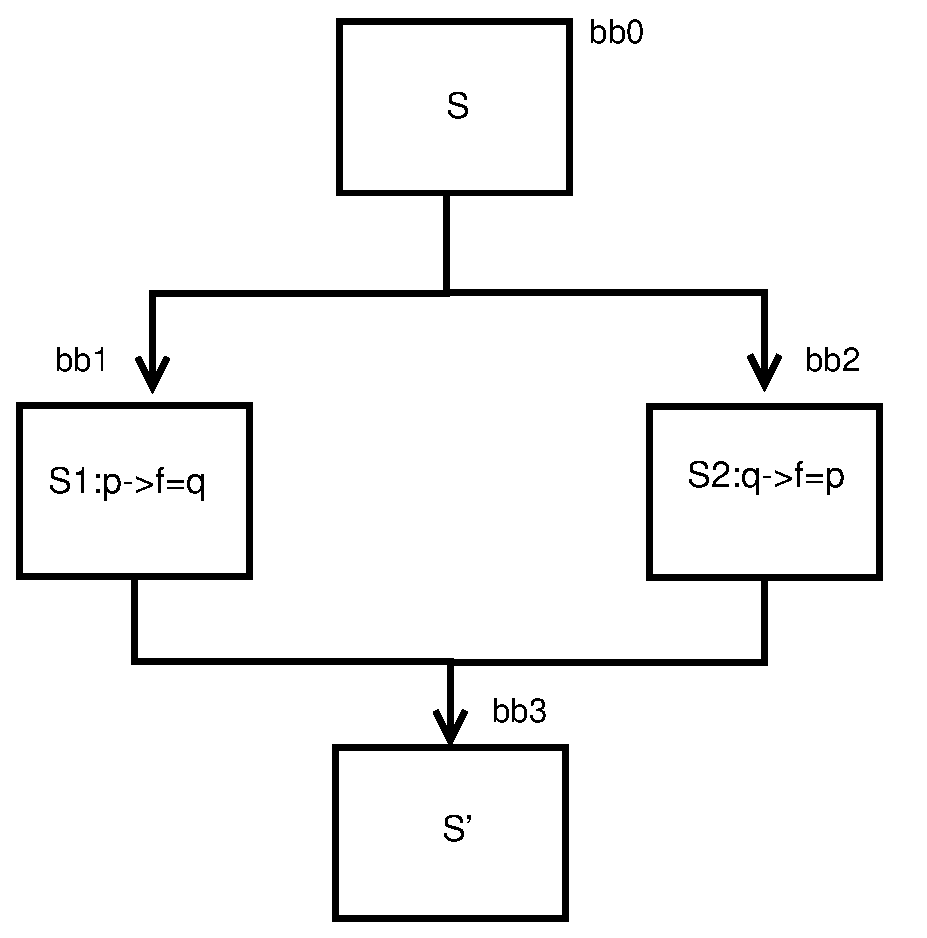
\includegraphics[scale=.4]{diagrams/Enhancements_d1.eps} & 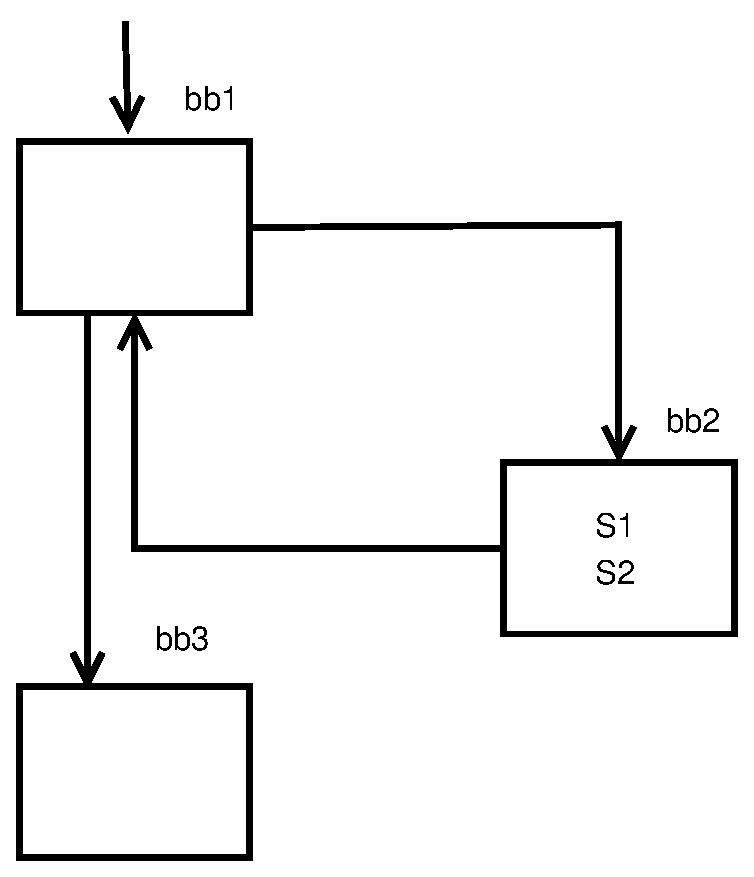
\includegraphics[scale=.4]{diagrams/Enhancements_d2.eps} \\
\footnotesize (a) & \footnotesize (b) 
\end{tabular}
\caption{CFG example}\label{CFG_1}
\end{figure}    


\subsection{Time optimization}
%We have just seen in the above subsection that there may be repetitions of
%terms in the boolean equaitons when conditional, looping or recursion is present in programs. Then why not remove the redundant terms in those 
%equations.Again here the time
%consumption is a problem,because manipulating strings as we know is a very costly operation.

% Because of this time constraint we haven't removed the redundant terms,
% but to reduce the computatuion time we have been hashing the results of these repeated terms.
Initially when we just stored the  boolean equation as it is and for that the  time taken for the analysis 
of merge\_recur to complete was \textbf{4 hrs}. But later we realized that, during the evaluation of boolean equation we are converting it to postfix, 
it is effective to store the postfix equation itself instead of infix. After this change the time for the analysis 
of merge\_recur reduced to \textbf{2 hrs}.

We have just seen in the above subsection that there may be repetitions of
terms in the boolean equations when conditional, looping or recursion is present in programs. Careful analysis of the equation for some sample programs 
made us notice that the time taken to evaluate these repeated terms can be cut down if we store their results in  some hash table and reuse 
whenever repetition occurs. This has reduced the time taken drastically, and the analysis of merge\_recur comes down to \textbf{35 seconds}.

\section{Testing Strategy}
We all know how important testing is in order to determine whether we are meeting our required results. In our analysis with the source code 
spanning close to 12000 LOC and a vast range of possible testcases, an efficient testing strategy is a must. 
  
We have written a script that could generate us many unit testcases depending on the number of statements that we want to have in our test case.
A sample template of how our testcase looks is presented in Program ~\ref{template}

\begin{figure}
\begin{lstlisting}[caption={Unit Testcase Template} ,label=template]
 
#include <stdlib.h>
int main()
{
	 typedef struct _node node;
	 struct _node {
		 node* f;
		 node* g;
	};

	 node* p = (node*)malloc(sizeof(node));
	 node* q = (node*)malloc(sizeof(node));

	/* HEAP MANIPULATION STARTS */
	.......
	.......
	/* HEAP MANIPULATION ENDS   */

}
\end{lstlisting}
\end{figure}
     
It is at those dotted lines that our pointer statements will be inserted. You could see in the template that the number of heap pointers are 2 and 
number of field pointer are 2.
With these properties the number of possibilities for each statement is 42, some of the possible statements are $\p \rightarrow \f =  \q$,$\p \rightarrow \g =  \q \rightarrow \f$, $\p \rightarrow \f = malloc() $, $\p = NULL$ and so on. If we increase the number of heap pointers or field pointers the 
possibilities for each statement would further increase.
The number of test cases generated for different number of statements is given in the Table.~\ref{TestCaseCount}
Once we have generated the testcases we run GHIYA's analysis and our analysis and compare the results for each. By comparison we mean comparing the shape 
of each pointer
after each GIMPLE statement.
Based on the comparison we put the test case in one of the three categories: PASS, SAFE, FAIL/ACCURATE. \\

\begin{itemize}
 \item PASS : GHIYA's analysis and our analysis gives the shape information at all statements
 \item SAFE : GHIYA's analysis is more accurate than us, .i.e for example if our analysis infers the shape as CYCLE, then Ghiya will
 infer more precise shapes like DAG or Tree.
 \item FAIL/ACCURATE : Our analysis gives less conservative shapes than GHIYA. If this happens then there could be two scenarios: 
 either we are giving accurate results or we are giving incorrect results. 
 All the testcases present in this case  are checked manually we ensure that we are not getting any fail cases.
\end{itemize}

\begin{table}
 \begin{center}
\begin{tabular}{|c|c|}
 \hline
 {\bf No Of Stmts} & {\bf TestCases Generated} \\ \hline
  1  & 42 \\ \hline
  2  & 1764 \\ \hline
  3  & 74088 \\ \hline 
\end{tabular}
\end{center}
\label{TestCaseCount}
\caption{No Of TestCases} 
\end{table}

\section{Results}
% \label{intro:community}

This section contains details about how would the Field sensitive analysis 
performs in terms of accuracy and performance when run on different benchmarks.
We also give results when this analysis is run on unit test cases. Every time we compare
the results with Ghiya method \cite{Ghiya96}. Ghiya's shape analysis is also
implemented as a GCC plugin which does context insensitive shape analysis.
First we will look at how the analysis performs on the unit test cases (about which we explained in earlier section)
and later we will show its performance on List benchmarks followed by one of the olden benchmark. The configuration of the machine used for
the generation of results are 2 GB RAM, Pentium Dual Core, 2.10Ghz. \\ \\
\textbf{Unit Test cases: }The details about these Unit Test cases are already given in the previous section.
All these test cases are compared with Ghiya's analysis.
Here  a comparison is done on how the results have varied before and after all the enhancements 
mentioned in Chapter 3 were included. They are given in the Table ~\ref{UnitRes}.

\begin{table}
 
\centering
\begin{tabular}{|c@{}|@{}c@{}|@{}c@{}|@{}c@{}|@{}c|}
 \hline
& TestCases & Pass & Safe & Accurate \\ \hline
Before \  & 
\begin{tabular}{c}
  ml-1 \\
  ml-2 \\
  ml-2-if \\
  ml-2-while \\
  ml-3
\end{tabular}
&
\begin{tabular}{c}
 42\\
 1572 \\
 1764 \\
 1108 \\
 51854
\end{tabular}
&
\begin{tabular}{c}
 0 \\
 24 \\
 0 \\
 452 \\
 6864
\end{tabular}
&
\begin{tabular}{c}
 0 \\
 168 \\
 0 \\
 204 \\
 15370
\end{tabular}
\\  \hline%----after
After & 
\begin{tabular}{c}
  ml-1 \\
  ml-2 \\
  ml-2-if \\
  ml-2-while \\
  ml-3 
\end{tabular}
&
\begin{tabular}{c}
  42\\
 1612 \\
 1764 \\
 1452 \\
 58444
\end{tabular}
&
\begin{tabular}{c}
 0\\
 0 \\
 0 \\
 0 \\
 0 
\end{tabular}
&
\begin{tabular}{c}
 0 \\
 152 \\
 0 \\
 312 \\
 16202
\end{tabular}
\\ \hline
\end{tabular}

\caption{Unit test cases results} \label{UnitRes}
\end{table}

   We have already mentioned about the script used to generate these unit test cases, these test cases can have any number of heap manipulation
statements as we desire. All those test cases with one heap manipulation are said to be ml-1, those with two as ml-2 etc.
Referring to template Program~\ref{template}, in the area where the heap manipulation statements are to be inserted, for ml-while and ml-if type test cases,  
while and if conditional statements are put. The template for these two are given below. The statement {\tt \p \ = null} was added just to find the
shape after these conditionals are executed. 

\begin{table}[h]
\centering
\begin{tabular}{ccc}
\begin{tabular}{l}
statement\_1 \\
while (condition)\{ \\
\ \ statement\_2 \\
\} \\
p = null; \\
\end{tabular}
& &

\begin{tabular}{l}
if (condition) \\
\ \ \ statement\_1 \\
else \\
\ \ \ statement\_2 \\
p = null; \\
\end{tabular}

\\ 
\footnotesize (a)ml-2-while & & \footnotesize (b)ml-2-if
\end{tabular}

\end{table}


The meaning of terms {\tt Safe},{\tt Pass},{\tt Accurate} are already explained in the previous section,but still just to reiterate.
\begin{itemize}
 \item {\tt Safe} : The shape inferred by Ghiya's analysis is more precise than that inferred by Sandeep's
 \item {\tt Accurate}: The shape inferred by Sandeep's analysis is more precise than that inferred by Ghiya's
 \item {\tt Pass} : The shape inferred is same by both the analysis.
\end{itemize}


When we look at the ml-2 results the number of {\tt Accurate} cases were more initially than there were after the enhancements. Though this was the case here we were able to
reduce the {\tt Safe} cases to 0 sacrificing some of the {\tt Accurate} cases. One such case is already mentioned in the Chapter~\ref{Enhancements}'s last part
about Information passed to successors. In ml-2-while there is a significant improvement in how the results turned out, the same can be noticed in ml-3. 

Now with all these changes we can say that in all these cases Sandeep's analysis is better than Ghiya's as there is not even a single safe case among all
of them. You can clearly understand this by seeing the entries of column {\tt Safe} which contains 0 throughout. \\ \\
\textbf{ List benchmarks}: We have also ran the analysis on Linked List benchmarks, source of which is \cite{linkedlist}. These benchmarks contains all the 
important operations that could be performed on linked list. 
We find the shape of each heap pointer at each basic statement, then we sum the number of times Tree's are detected, similarly number of times Dag's and Cycle's are
detected. This triple (Tree,Dag,Cycle) is used for comparison of results.

\begin{table}[htbp]
\scalebox{0.90}{
\begin{tabular}{|l|l|c|l|c|c|}
\hline
\multicolumn{ 1}{|c|}{Benchmark} & \multicolumn{ 2}{c|}{Ghiya's Analysis} & \multicolumn{ 2}{c|}{Field Sensitive} & \multicolumn{ 1}{l|}{Result} \\ \cline{ 2- 5}
\multicolumn{ 1}{|c|}{} & Shape & \multicolumn{1}{l|}{Time(Sec)} & Shape & \multicolumn{1}{l|}{Time(Sec)} & \multicolumn{ 1}{l|}{} \\ \hline
100\_create\_iter.cpp & (30,0,0) & 0 & (30,0,0) & 0.179 &  \\ \hline
100\_create\_recur.cpp & (36,0,0) & 0 & (22,0,14) & 0.147 & \# \\ \hline
200\_delall\_iter\_create\_fixed.cpp & (168,0,0) & 0 & (168,0,0) & 1.385 &  \\ \hline
200\_delall\_iter\_create\_iter.cpp & (63,0,0) & 0 & (63,0,0) & 0.644 &  \\ \hline
200\_delall\_recur\_create\_fixed.cpp & (12,0,0) & 0 & (12,0,0) & 0.093 &  \\ \hline
200\_delall\_recur\_create\_iter.cpp & (56,0,0) & 0 & (56,0,0) & 0.502 &  \\ \hline
300\_insert\_iter\_create\_fixed.cpp & (341,19,0) & 0.002 & (343,17,0) & 8.945 & \$ \\ \hline
300\_insert\_iter\_create\_iter.cpp & (161,19,0) & 0.002 & (163,17,0) & 5.018 & \$ \\ \hline
300\_insert\_recur\_create\_fixed.cpp & (225,0,27) & 0.001 & (225,0,27) & 3.147 &  \\ \hline
300\_insert\_recur\_create\_iter.cpp & (113,0,27) & 0.001 & (113,0,27) & 2.266 &  \\ \hline
400\_remove\_iter\_create\_fixed.cpp & (314,0,26) & 0.001 & (318,22,0) & 3.787 & \$ \\ \hline
400\_remove\_iter\_create\_iter.cpp & (154,0,26) & 0.001 & (177,3,0) & 3.363 & \$ \\ \hline
400\_remove\_recur\_create\_fixed.cpp & (243,0,18) & 0.001 & (234,0,27) & 2.932 & \# \\ \hline
400\_remove\_recur\_create\_iter.cpp & (108,0,18) & 0.001 & (99,0,27) & 1.766 & \# \\ \hline
500\_search\_iter\_create\_fixed.cpp & (168,0,0) & 0 & (168,0,0) & 1.225 &  \\ \hline
500\_search\_iter\_create\_iter.cpp & (63,0,0) & 0 & (63,0,0) & 0.596 &  \\ \hline
500\_search\_recur\_create\_fixed.cpp & (208,0,0) & 0 & (208,0,0) & 2.123 &  \\ \hline
500\_search\_recur\_create\_iter.cpp & (88,0,0) & 0 & (88,0,0) & 1.229 &  \\ \hline
600\_append\_iter\_create\_fixed.cpp & (358,6,0) & 0.002 & (349,15,0) & 4.462 & \# \\ \hline
600\_append\_iter\_create\_iter.cpp & (163,6,0) & 0.001 & (154,15,0) & 3.239 & \# \\ \hline
600\_append\_recur\_create\_fixed.cpp & (354,0,38) & 0.002 & (342,0,50) & 5.641 & \# \\ \hline
600\_append\_recur\_create\_iter.cpp & (144,0,38) & 0.002 & (132,0,50) & 3.886 & \# \\ \hline
700\_merge\_iter\_create\_fixed.cpp & (311,0,109) & 0.005 & (311,0,109) & 670.033 &  \\ \hline
700\_merge\_iter\_create\_iter.cpp & (242,0,142) & 0.007 & (242,0,142) & 318.464 &  \\ \hline
700\_merge\_recur\_create\_fixed.cpp & (498,0,114) & 0.006 & (498,0,114) & 33.446 &  \\ \hline
700\_merge\_recur\_create\_iter.cpp & (228,0,114) & 0.006 & (228,0,114) & 22.446 &  \\ \hline
800\_reverse\_iter\_create\_fixed.cpp & (233,0,47) & 0.001 & (241,0,39) & 7.179 & \$ \\ \hline
800\_reverse\_iter\_create\_iter.cpp & (83,0,47) & 0.001 & (91,0,39) & 3.707 & \$ \\ \hline
800\_reverse\_recur\_create\_fixed.cpp & (499,0,62) & 0.004 & (489,0,72) & 13.408 & \$ \\ \hline
800\_reverse\_recur\_create\_iter.cpp & (244,0,62) & 0.003 & (234,0,72) & 8.285 & \$ \\ \hline
\end{tabular}
}

\centering{ \$-Field sensitive analysis is more precise  \quad  \#- Ghiya's analysis is more precise}
\caption{Comparison On List Benchmark}
\label{listres}
\end{table}



% \begin{table}[htbp]
% \scalebox{0.90}{
% \begin{tabular}{|l|l|c|l|c|c|}
% \hline
% \multicolumn{ 1}{|c|}{Benchmark} & \multicolumn{ 2}{c|}{Ghiya's Analysis} & \multicolumn{ 2}{c|}{Field Sensitive} & \multicolumn{ 1}{l|}{Result} \\ \cline{ 2- 5}
% \multicolumn{ 1}{|c|}{} & Shape & \multicolumn{1}{l|}{Time(Sec)} & Shape & \multicolumn{1}{l|}{Time(Sec)} & \multicolumn{ 1}{l|}{} \\ \hline
% 100\_create\_iter.cpp & (30,0,0) & 0.003 & (30,0,0) & 0.25 & * \\ \hline
% 100\_create\_recur.cpp & (36,0,0) & 0.003 & (22,0,14) & 0.198 & \# \\ \hline
% 200\_delall\_iter\_create\_iter.cpp & (63,0,0) & 0.006 & (63,0,0) & 0.861 & * \\ \hline
% 200\_delall\_recur\_create\_fixed.cpp & (12,0,0) & 0.002 & (12,0,0) & 0.119 & * \\ \hline
% 300\_insert\_iter\_create\_fixed.cpp & (69,11,0) & 0.027 & (71,9,0) & 1.874 & \$ \\ \hline
% 300\_insert\_recur\_create\_fixed.cpp & (225,0,27) & 0.013 & (225,0,27) & 3.87 & * \\ \hline
% 400\_remove\_iter\_create\_fixed.cpp & (348,0,26) & 0.012 & (352,22,0) & 4.854 & \$ \\ \hline
% 400\_remove\_recur\_create\_fixed.cpp & (243,0,18) & 0.013 & (234,0,27) & 3.598 & \# \\ \hline
% 500\_search\_iter\_create\_fixed.cpp & (168,0,0) & 0.007 & (168,0,0) & 1.587 & * \\ \hline
% 500\_search\_recur\_create\_fixed.cpp & (208,0,0) & 0.008 & (208,0,0) & 2.579 & * \\ \hline
% 600\_append\_iter\_create\_fixed.cpp & (358,6,0) & 0.02 & (349,15,0) & 5.697 & \# \\ \hline
% 600\_append\_recur\_create\_fixed.cpp & (354,0,38) & 0.024 & (342,0,50) & 6.751 & \# \\ \hline
% 700\_merge\_iter\_create\_fixed.cpp & (311,0,109) & 0.069 & (311,0,109) & 664.56 & * \\ \hline
% 700\_merge\_recur\_create\_fixed.cpp & (498,0,114) & 0.079 & (498,0,114) & 42.63 & * \\ \hline
% 800\_reverse\_iter\_create\_fixed.cpp & (233,0,47) & 0.013 & (241,0,39) & 8.881 & \$ \\ \hline
% 800\_reverse\_recur\_create\_fixed.cpp & (499,0,62) & 0.041 & (489,0,72) & 18.346 & \# \\ \hline
% \end{tabular}
% }
% \label{ListRes}
% \caption{Comparision On List Benchmark}
% \centering{*- Same Result  \quad \$- Precise Result \quad  \#- Ghiya's result is more precise}
% \end{table}





% \begin{table}[htbp]
% \caption{Comparison On List Benchmark}
% \begin{tabular}{|l|l|l|l|l|}
% \hline
% \multicolumn{ 1}{|c|}{Benchmark} & \multicolumn{ 2}{l|}{Ghiya's Analysis} & \multicolumn{ 2}{l|}{Sandeep's Analysis} \\ \cline{ 2- 5}
% \multicolumn{ 1}{|c|}{} & Shape & \multicolumn{1}{l|}{Time(Sec)} & Shape & Time(Sec) \\ \hline
% 100\_create\_iter.cpp & (30,0,0) & 0.002 & (30,0,0) & 0.324 \\ \hline
% \red{100\_create\_recur.cpp} & (36,0,0) & 0.004 & (22,0,14) & 0.189 \\ \hline
% 200\_delall\_iter\_create\_iter.cpp & (63,0,0) & 0.01 & (63,0,0) & 1.479 \\ \hline
% 200\_delall\_recur\_create\_fixed.cpp & (12,0,0) & 0.004 & (12,0,0) & 0.144 \\ \hline
% \red{300\_insert\_iter\_create\_fixed.cpp} & (69,11,0) & 0.01 & (71,7,2) & 2.248 \\ \hline
% 300\_insert\_recur\_create\_fixed.cpp & (228,0,24) & 0.01 & (228,0,24) & 4.082 \\ \hline
% \blue{400\_remove\_iter\_create\_fixed.cpp} & (351,0,23) & 0.011 & (355,19,0) & 4.692 \\ \hline
% \red{400\_remove\_recur\_create\_fixed.cpp} & (245,0,16) & 0.01 & (237,0,24) & 3.485 \\ \hline
% 500\_search\_iter\_create\_fixed.cpp & (168,0,0) & 0.006 & (168,0,0) & 1.455 \\ \hline
% 500\_search\_recur\_create\_fixed.cpp & (208,0,0) & 0.007 & (208,0,0) & 2.57 \\ \hline
% \blue{600\_append\_iter\_create\_fixed.cpp} & (343,0,21) & 0.019 & (351,9,4) & 5.347 \\ \hline
% 600\_append\_recur\_create\_fixed.cpp & (355,0,37) & 0.022 & (355,0,37) & 6.639 \\ \hline
% 700\_merge\_iter\_create\_fixed.cpp & (320,0,100) & 0.044 & (320,0,100) & 1033.317 \\ \hline
% \blue{700\_merge\_recur\_create\_fixed.cpp} & (506,0,106) & 0.054 & (508,0,104) & 43.832 \\ \hline
% \blue{800\_reverse\_iter\_create\_fixed.cpp} & (233,0,47) & 0.015 & (241,0,39) & 8.997 \\ \hline
% \blue{800\_reverse\_recur\_create\_fixed.cpp} & (429,0,132) & 0.064 & (561,0,0) & 6.805 \\ \hline
% \end{tabular}
% \label{ListRes}
% \end{table}
  
  
The results are present in Table ~\ref{listres}. The last column tells whether the field sensitive performs better than Ghiya's analysis or not in the particular benchmark.
A blank entry means that both gave the same results. Also the meaning of $\$$ and $\#$ are explained in the table. \\ \\ 
\begin{table}[h]
\centering
\begin{tabular}{|l|l|c|l|c|c|}
\hline
\multicolumn{ 1}{|c|}{Benchmark} & \multicolumn{ 2}{c|}{Ghiya's Analysis} & \multicolumn{ 2}{c|}{Field Sensitive} & \multicolumn{ 1}{l|}{Result} \\ \cline{ 2- 5}
\multicolumn{ 1}{|c|}{} & Shape & \multicolumn{1}{l|}{Time(Sec)} & Shape & \multicolumn{1}{l|}{Time(Sec)} & \multicolumn{ 1}{l|}{} \\ \hline
TreeAdd & (63,0,0) & 0.001 & (30,0,24) & 1.2 & \# \\ \hline
\end{tabular}
\caption{Olden: TreeAdd benchmark}
\label{OldenRes}
\end{table}
\textbf{Olden Benchmarks \cite{Olden}}: We ran the analysis on the benchmark TreeAdd, there are several other benchmarks which belong to this set, but due to the problem of
large memory consumption we were not able to run those benchmarks. Results on this benchmark are given in Table ~\ref{OldenRes}.\\ \\
As you can see there are eight of List benchmarks where the results are better than Ghiya's analysis. Also there are seven List benchmarks and the TreeAdd benchmark for which the results are not as good as Ghiya.
The main reason for the reduction in the preciseness is the dummy statement. As this statement doesn't kill any information, summarization of nodes takes
place. It means that a pointer will be having having data flow values about more than one node. Some of the recursive benchmarks like create\_recur and remove\_recur 
when ran on context sensitive interprocedural analysis, gave results same as that of Ghiya, but we were not able to run it on all of the benchmarks because of excessive memory consumption. 
If we could come up with a memory efficient context sensitive analysis the results would surely improve.

Coming to the time taken, we evaluate the boolean equation of each heap pointer and each basic statement; and as the size of the boolean equations also
can be large, the time it takes is much more compared to other analysis. Still effort is needed to reduce this by finding any optimizations possible or change the
way the boolean equations are represented. 



\chapter{Conclusion and Future Work\label{Conclusion}}
% \section{Conclusion}

In this report we have suggested several enhancements to Sandeep's work on Field Sensitive analysis
which ensure the correctness and increase the accuracy of the analysis.
Now after these changes the analysis is better than Ghiya's work in all those unit test cases described. 
We have also introduced a new analysis called subset based analysis which infers shape based on the subset of fields actually accessed inside
a function. This helps us inferring information like a function is traversing/accessing a tree substructure of a cyclic data structure. 
We also proposed a shape sensitive inter procedural
analysis which is in mid way of context sensitive and context insensitive analysis and could possibly balance the memory consumption and 
preciseness at the same time. We have also performed various 
optimizations with the aim of decreasing the memory consumption and time for completion.
The testing strategy used is exhaustive and has helped a lot in identifying the cases of safe and incorrect results.

There are some benchmarks where the results are not as good as Ghiya's, these are due to the
summarization of heap nodes due to the dummy statement. In the future we plan to work on
this issue.
The analysis has concerns over the amount of memory it takes even after the optimizations performed. We want
to address this concern by representing boolean equations in much efficient way. 
% The callstring approach is using
% more memory for this analysis, so we plan to find out some other context sensitive analysis which is
% memory efficient.

% \section{Future Work}
% Representation of boolean equations in a memory efficient
% Better memory efficient Context sensitive analysis
% Extend this for arrays of pointers




\appendix
\chapter[Analysis of Ghiya]{Analysis of Ghiya ~\cite{Ghiya96}\footnote{The contents of this section are borrowed from ~\cite{Ghiya96}}}
\appendix
%%%%%%%%%%%%%%%%%%%%%%%%%%%%%%%%%%%%%%%%%%%%%%%%%%%%%%%%%%%%%%%%%%%%%%
\chapter[Analysis of Ghiya et. al.~\cite{Ghiya96}]{Analysis of Ghiya et. al.~\cite{Ghiya96}\footnote{The contents of this section are borrowed from ~\cite{Ghiya96}}}
%%%%%%%%%%%%%%%%%%%%%%%%%%%%%%%%%%%%%%%%%%%%%%%%%%%%%%%%%%%%%%%%%%%%%%
Most of the definitions and technical terms used in this chapter are borrowed from the aforementioned paper.
The proposed shape analysis composed of three store-less
abstractions that are computed together at each program point.
For each heap directed pointer they approximated the attribute
shape and for each pair of heap directed pointers they approximated the 
direction and interference relationships between them. These three abstractions 
are defined formally as follows:

\begin{definition}
Given any heap-directed pointer $p$, the shape attribute p.shape is Tree, 
if in the data structure accessible from p there is a unique (possibly empty) access path 
between any two nodes (heap objects) belonging to it. It is considered to be DAG (directed acyclic graph), 
if there can be more than one path between any two nodes in this data structure, 
but there is no path from a node to itself (i. e, it is acyclic). 
If the data structure contains a node having a path to itself, p.shape is considered to be Cycle.
Note that as lists are special case of tree data structures, their shape is also considered as Tree.
\end{definition}

\begin{definition}
Given two heap directed pointers $p$ and $q$, the direction matrix $D$ captures the following 
relationships between them:
\begin{itemize}
\item $D[p,q] = 1 : $ An access path possibly exists in the heap, from the heap object pointed to by $p$,
to the heap object pointed to by $q$. In this case we simply say that the pointer $p$ has a path to 
pointer $q$.
\item $D[p,q] = 0 : $ No access path exists from the heap object pointed to by $p$ to the heap object pointed to by $q$. 
\end{itemize}
\end{definition}

\begin{definition}
Given two heap directed pointers $p$ and $q$, the direction matrix $I$ captures the following 
relationships between them:
\begin{itemize}
\item $I[p,q] = 1 : $ A common heap object can be possibly accessed starting from pointers $p$ and $q$.
In this case we state that pointers $p$ and $q$ can interfere.
\item $I[p,q] = 0 : $ No common heap object can be accessed starting from pointers $p$ and $q$.
In this case we state that pointers $p$ and $q$ do not interfere.
\end{itemize}
\end{definition}

Direction relationships are used to actually estimate the shape attributes, where the interference 
relationships are used for safely calculating direction relationships. 

\subsection*{Illustrative Example}

The direction and interference matrices are illustrated in Fig.~\ref{fig:relwork_1}.
Part (a) represents a heap structures at a program point, while parts (b) and (c) show the direction 
and interference matrices for it.  
\begin{figure}
\centering
\begin{tabular}{c@{$\qquad\qquad$}c}
\multicolumn{2}{c}{
\scalebox{0.80} { 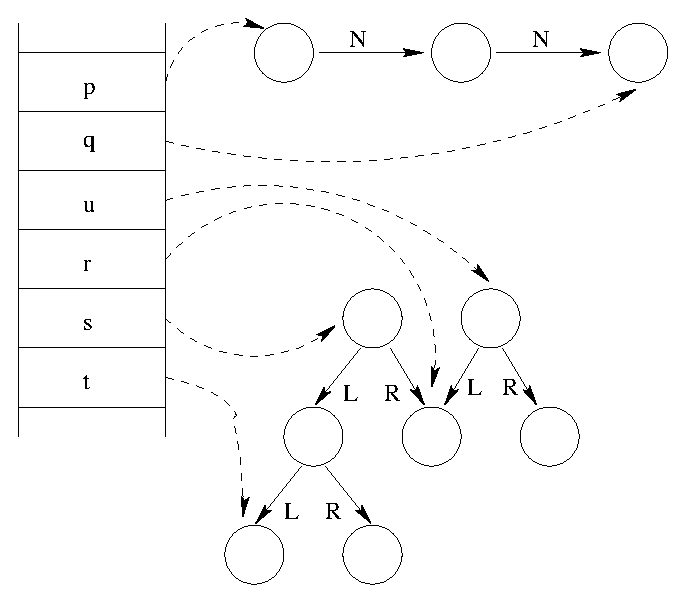
\includegraphics[scale=1]{diagrams/Appendix_2.eps}}
} \\
\multicolumn{2}{c}{
\scalebox{0.80}{ (a) Heap Structure }
} \\ \\
\scalebox{0.80} { \begin{tabular}{|c||c|c|c|c|c|c|}
\hline
$D$ & $p$ & $q$ & $r$ & $s$ & $t$ & $u$ \\ \hline \hline
$p$ & $1$ & $1$ & $0$ & $0$ & $0$ & $0$ \\ \hline 
$q$ & $0$ & $1$ & $0$ & $0$ & $0$ & $0$ \\ \hline 
$r$ & $0$ & $0$ & $1$ & $0$ & $0$ & $0$ \\ \hline 
$s$ & $0$ & $0$ & $1$ & $1$ & $1$ & $0$ \\ \hline 
$t$ & $0$ & $0$ & $0$ & $0$ & $1$ & $0$ \\ \hline 
$u$ & $0$ & $0$ & $1$ & $0$ & $0$ & $1$ \\ \hline 
\end{tabular}} 
& 
\scalebox{0.80} {\begin{tabular}{|c||c|c|c|c|c|c|}
\hline
$I$ & $p$ & $q$ & $r$ & $s$ & $t$ & $u$ \\ \hline \hline
$p$ & $1$ & $1$ & $0$ & $0$ & $0$ & $0$ \\ \hline 
$q$ & $1$ & $1$ & $0$ & $0$ & $0$ & $0$ \\ \hline 
$r$ & $0$ & $0$ & $1$ & $1$ & $0$ & $1$ \\ \hline 
$s$ & $0$ & $0$ & $1$ & $1$ & $1$ & $1$ \\ \hline 
$t$ & $0$ & $0$ & $0$ & $1$ & $1$ & $0$ \\ \hline 
$u$ & $0$ & $0$ & $1$ & $1$ & $0$ & $1$ \\ \hline 
\end{tabular}}  \\
\scalebox{0.80}{ (b) Direction Matrix}  & \scalebox{0.80} {(c) Interference Matrix}
\end{tabular}
\caption{Example Direction and Interference Matrices}
\label{fig:relwork_1}
\end{figure}


We now demonstrate how direction relationships help estimate the shape of the data structures.
In Fig.~\ref{fig:relwork_2}, initially we have both \p.\shape\ and \q.\shape\ as Tree. Further $D[q,p] == 1$, as there 
exists a path from \q\ to \p\ through {\tt next} link. The statement {\tt p$\rightarrow$prev = q}, sets up a path from
\p\ to \q\  through the {\tt prev} link. From direction matrix information we already know that a path exists
from \q\ to \p, and now a path is being set from \p\ to \q. Thus after the statement, $D[p,q] = 1$, $D[q,p] = 1$, \p.\shape\ = Cycle
and \q.\shape\ = Cycle.  

\begin{figure}
\centering
\scalebox{.80} {
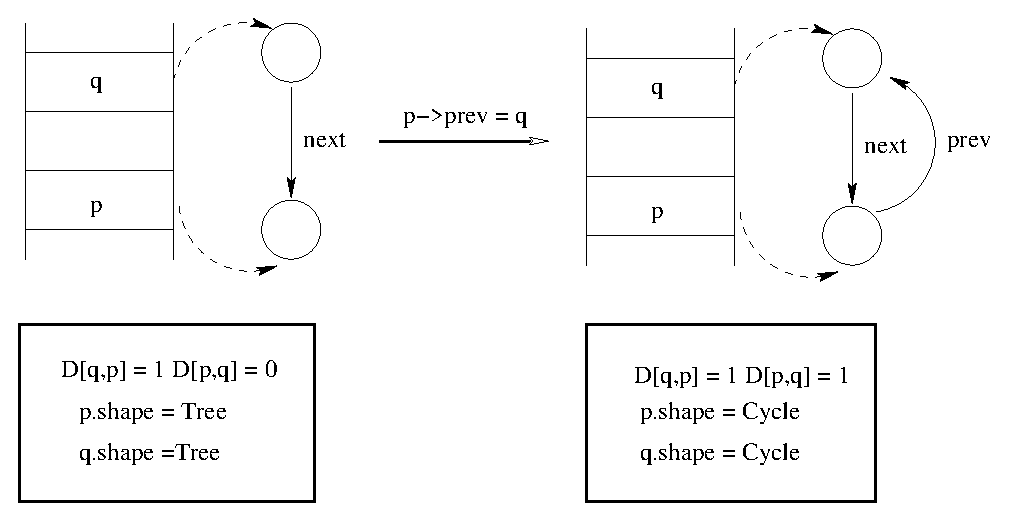
\includegraphics[scale=1]{Figure/figure_3}
}
\caption{Example Demonstrating Shape Estimation}
\label{fig:relwork_2}
\end{figure}

\subsection*{Analysis of Basic Statements}
They have considered eight basic statements that can access or
modify heap data structures as listed in Fig.~\ref{fig:relwork_3}(a). Variables \p\ and \q and the field $f$ are
of pointer type, variable $k$ is of integer type, and $op$ denotes the $+$ and $-$ operations. The 
overall structure of the analysis is shown in Fig.~\ref{fig:relwork_3}(b). Given the direction and the interference 
matrices $D$ and $I$ at a program point x, before the given statement, they compute the matrices $D_n$ and $I_n$
at a program point y. Additionally, we have the attribute matrix A, where for a pointer $p$, $A[p]$ gives its shape attribute.
The attribute matrix after the statement is presented as $A_n$.

For each statement they compute the set of direction and interference relationships it kills and generates. Using these sets, the
new matrices $D_n$ and $I_n$ are computed as shown in Fig.~\ref{fig:relwork_3}(c). Note that the elements in the gen and kill sets are denoted as $D[p,q]$
for direction relationships, and $I[p,q]$ for interference relationships. Thus a gen set of the form $\{D[x,y], D[y,z]\}$, indicates that
the corresponding entries in the output direction matrix $D_n[x,y]$ and $D_n[y,z]$ should be set to one. We also compute the set of 
pointers $H_s$, whose shape  attribute can be modified by the given statement. Another attribute matrix $A_c$ is used to store the 
changed attribute of pointers belonging to the set $H_s$. The attribute matrix $A_n$ is then computed using the 
matrices $A$ and $A_c$ as shown in Fig.~\ref{fig:relwork_3}(c).  

Let $H$ be the set of pointers whose relationships/attributes are abstracted by the matrices $D$. $I$ and $A$. Further
assume that updating an interference matrix entry $I[\q,\p]$, implies identically updating the entry $I[\p,\q]$.   
\begin{figure}
\centering
\scalebox{0.90}{
\begin{tabular}{|c|c|c|}
\hline
\begin{tabular}{l}
Allocation \\
1. {\tt p = malloc();} \\
\\
Pointer Assignments \\
2. {\tt p = q;} \\
3. {\tt p = \&(q$\rightarrow$f);} \\
4. {\tt p = q op k;} \\
5. {\tt p = NULL;} \\
6. {\tt p = q$\rightarrow$f;} \\
\\
Structure Updates \\
7. {\tt p$\rightarrow$f = q;} \\
8. {\tt p$\rightarrow$f = NULL;}
\end{tabular}  &
\begin{tabular}{c}
\scalebox{0.80}{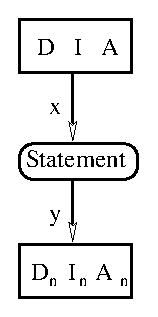
\includegraphics[scale=1]{diagrams/Appendix_4.eps}}
\end{tabular}
&
\begin{tabular}{l}
Build the new matrices\\
$\begin{array}{lll} 
\forall r,s \in H, & D_n[r,s] = D[r,s], & I_n[r,s] = I[r,s] \\
\forall s \in H, & A_n[s] = A[s]
\end{array}$ \\
\\
Delete Killed relationships \\
$\begin{array}{ll} 
\forall entries\ D[r,s] \in D\_kill\_set, & D_n[r,s] = 0\\  
\forall entries\ I[r,s] \in I\_kill\_set, & I_n[r,s] = 0\\  
\end{array}$ \\
\\
Add generated relationships \\
$\begin{array}{ll} 
\forall entries\ D[r,s] \in D\_gen\_set, & D_n[r,s] = 1\\  
\forall entries\ I[r,s] \in I\_gen\_set, & I_n[r,s] = 1\\  
\end{array}$ \\
\\
Update shape attributes of affected pointers \\
Compute $H_s$ and $A_s$ \\
$\begin{array}{ll} 
\forall s \in H_s, & A_n[s] = A[s]\\  
\end{array}$
\end{tabular}
\\
\scalebox{0.80}{(a) Basic statements} & \scalebox{0.80}{(b) Analysis Structure} & \scalebox{0.80}{(c) General Form of Analysis Rules} \\
\hline
\end{tabular}
}
\caption{The Overall Struture of the Analysis}
\label{fig:relwork_3} 
\end{figure}


The actual analysis rules can be divided into three groups: (1) allocations, (2) pointer assignments, and 
(3) structure updates. Figure~\ref{fig:relwork_4} shows the gen and kill sets corresponding to each statement. 
\begin{figure}[h]
\centering
\begin{tabular}{|l|c|}
\hline
1. {\tt p  = malloc();} &  
					$\begin{array}{lll}
						D\_kill\_set &=& \{D[p,s] \vert s \in H \wedge D[p,s]\}\ \cup\\
                                     &&   \{D[s,p] \vert s \in H \wedge D[s,p]\} \\
						I\_kill\_set &=& \{I[p,s] \vert s \in H \wedge I[p,s]\} \\
						D\_gen\_set &=& \{D[p,p]\} \quad I\_gen\_set = \{I[p,p]\} \\
						H_s &=& \{p\} \quad A_c[p] = Tree 	\\
					\end{array}$
								\\
\hline
\begin{tabular}{l}
2. {\tt p = q;} \\
3. {\tt p = \&(q$\rightarrow$f);} \\
4. {\tt p = q op k;} \\
\end{tabular}
 & 
				\begin{tabular}{l}
					Kill set same as that of {\tt p  = malloc();} \\
					$\begin{array}{lll}
						D\_gen\_set\_from &=& \{D[s,p] \vert s \in H \wedge s \not= p \wedge D[s,q]\} \\
						D\_gen\_set\_to &=& \{D[p,s] \vert s \in H \wedge s \not= p \wedge D[q,s]\} \\
						I\_gen\_set	&=& \{I[p,s] \vert s \in H \wedge s \not= p \wedge I[q,s]\}\ \cup \\
											&&  \{I[p,p] \vert I[q,q]\} \\
						D\_gen\_set	&=& D\_gen\_set\_from\ \cup D\_gen\_set\_to \\
						H_s &=& \{p\} \quad A_c[p] = A[q] 	\\
					\end{array}$
				\end{tabular}
								\\
\hline
5. {\tt p = NULL;} & 
				\begin{tabular}{l}
					Kill set same as that of {\tt p  = malloc();} \\
					$\begin{array}{lll}
						D\_gen\_set &=& \{\} \quad I\_gen\_set = \{\} \\
						H_s &=& \{p\} \quad A_c[p] = Tree 	\\
					\end{array}$
				\end{tabular}
								\\
\hline
6. {\tt p = q$\rightarrow$f;} & 
				\begin{tabular}{l}
					Kill set same as that of {\tt p  = malloc();} \\
					$\begin{array}{lll}
						D\_gen\_set\_from 	&=& \{D[s,p] \vert s \in H \wedge s \not= p \wedge I[s,q]\} \\
						D\_gen\_set\_to 	&=& \{D[p,s] \vert s \in H \wedge s \not= p \wedge s \not= q\ \wedge \\
                                            &&    D[q,s]\}\ \cup \{D[p,q] \vert A[q] = Cycle\}\ \cup \\
											&& \{D[p,p] \vert D[q,q]\} \\
						D\_gen\_set 		&=& D\_gen\_set\_from\ \cup D\_gen\_set\_to \\
						I\_gen\_set 		&=& \{I[p,s] \vert s \in H \wedge s \not= p \wedge I[q,s]\}\ \cup \\
											&&  \{I[p,p] \vert I[q,q]\} \\
						A_c[p] &=& A[q] 	\\
					\end{array}$
				\end{tabular}
								\\
\hline
7. {\tt p$\rightarrow$f = NULL;} & 
					$\begin{array}{lll}
						D\_kill\_set &=& \{\} \quad I\_kill\_set = \{\}\\
						D\_gen\_set 		&=& \{\} \quad I\_gen\_set  = \{\}\\
						A_c[p] &=& A[p]\ \forall p \in H  	\\
					\end{array}$
								\\
\hline
7. {\tt p$\rightarrow$f = q;} & 
				\begin{tabular}{l}
					Kill set same as that of {\tt p$\rightarrow$f = NULL;} \\
					$\begin{array}{lll}
						D\_gen\_set		&=& \{D[r,s] \vert r,s \in H \wedge D[r,p] \wedge D[q,s]\}  \\
						I\_gen\_set  	&=& \{I[r,s] \vert r,s \in H \wedge D[r,p] \wedge I[q,s]\} \\
					\end{array}$ \\ \\
					\underline{Pointer q already has a path to p, D[q,p] = 1} \\
					$\begin{array}{lll}
						H_s 			&=& \{s \vert s \in H \wedge (D[s,p] \vee D[s,q])\} \\
						D[q,p] &\Rightarrow& A_c[s] = Cycle\ \forall s \in H_s  	\\
					\end{array}$ \\ \\
					\underline{A[q] = Tree} \\
					$\begin{array}{lll}
						H_s 			&=& \{s \vert s \in H \wedge (D[s,p] \vee I[s,q])\} \\
						(\neg D[q,p] \wedge (A[q] = Tree)) &\Rightarrow& A_c[s] = A[s] \Join Dag\ \forall s \in H_s  	\\
					\end{array}$ \\ \\
					\underline{A[q] $\not=$ Tree} \\
					$\begin{array}{lll}
						H_s 			&=& \{s \vert s \in H \wedge D[s,p]\} \\
						(\neg D[q,p] \wedge (A[q] \not= Tree)) &\Rightarrow& A_c[s] = A[s] \Join A[q]\ \forall s \in H_s  	\\
					\end{array}$
				\end{tabular}
								\\
\hline							
\end{tabular}
\caption{Analysis Rules}
\label{fig:relwork_4}
\end{figure}


%%%%%%%%%%%%%%%%%%%%%%%%%%%%%%%%%%%%%%%%%%%%%%%%%%%%%%%%%%%%%%%%%%%%%%
\chapter[Analysis of Marron et. al.~\cite{marron06static}]{Analysis of Marron et. al.~\cite{marron06static}\footnote{The contents of this section are borrowed from ~\cite{marron06static}}}
%%%%%%%%%%%%%%%%%%%%%%%%%%%%%%%%%%%%%%%%%%%%%%%%%%%%%%%%%%%%%%%%%%%%%%
Most of the technical terms used in this chapter are borrowed from the aforementioned paper.
The proposed analysis followed the abstract heap graph model that uses nodes to
represent sets of concrete cells (heap allocated objects and arrays) and edges to represent sets of pointers. 
Each node in the abstract heap graph can be viewed as a region in memory on which certain
layout predicates can be defined (Tree Layout, List Layout, Singleton Layout, Multi-Path or Cycle Layouts)
which signifies what types traversal patterns a program can use to navigate through the data
structures in the region. To track the concrete Structure Layout, they introduce a simple domain of 
layout types = \{Singleton, List, Tree, Multi-Path, Cycle\}. The abstract layouts can be given a simple
total order: Singleton < List < Tree < Multi-Path < Cycle. This order can be interpreted as: if
a node n has abstract layout $\zeta$ then the concrete region, $\mathcal{R} = \gamma(n)$, where $\gamma$ is the concreatization
operator, may have any of the layout properties less than or equal to $\zeta$. For example, if we have a node
with layout type List the concrete region may have the List or Singleton layout properties. If the
node has Cycle as the layout then the concrete domain may have any of the layout properties. The
abstract layout for a node n represents the most general concrete layout that may be encountered
by a program traversing the region that is represented by the node n.

In their analysis, sometimes refinement is necessary (after summarization the abstract heap graph) whose 
purpose is to transform summary representations into forms that make certain relationships explicit, so that the information
 in these relationships can be utilized more easily. During refinement they turn summary nodes 
into a number of nodes of size one so that strong updates can be performed and exact relations 
between variables can be maintained. 

In order to eliminate the state explosion that is possible with refinement, they adopt the approach
of only doing refinement in those cases in which we can be sure that there is a unique way in which
new nodes can be materialized. This limits the level of details that can be achieved, but it 
is easy to demonstrate scenarios where refinement into multiple possibilities is needed to get results with the
desired accuracy. 


\addcontentsline{toc}{chapter}{References}
\bibliographystyle{alpha}
\bibliography{References}


\end{document}
%*******************************************************************************
